\documentclass[oneside]{ctexbook}
% oneside openright 消除空白页
\usepackage{geometry}
\usepackage{natbib}
\usepackage{booktabs}
\usepackage{hyperref} 
\usepackage{amsmath}
\usepackage{amsfonts}
\usepackage{eucal}
\usepackage{cancel}
\usepackage{amssymb}
\usepackage{calligra}
\usepackage{multirow}
\usepackage{bm}
\usepackage{graphicx}
\usepackage{subfigure}
\usepackage{float}
\usepackage{pgf,tikz,pgfplots}
\pgfplotsset{compat=1.15}
\usepackage{mathrsfs}
\usetikzlibrary{arrows}
\usepackage[textfont=bf]{caption}
\hypersetup{hidelinks}
\geometry{a4paper,scale=0.8}
\title{二维多铁材料设计}
\author{Dogcraft}

\begin{document}

\maketitle
\chapter*{摘要}

    多铁材料是指在一个单一的相之中存在一个以上的铁性质的材料,铁性质是指例如铁磁、铁电、铁弹性等性质,这些铁性质之中,最具备理论与应用价值的是铁电与铁磁这两个重要的经典性质,也是目前凝聚态物理研究的热点,目前通常指代将铁磁性行为与铁电相结合的电磁材料。
    多铁材料的研究范围也逐渐宽展到了二维材料领域,二维多铁材料研究的方法与一般的多铁材料相同。二维材料在空间结构上与三维体材料的巨大差别使得二维材料出现了很多新奇的物理特性。二维铁磁、铁电材料十分少见,二维多铁材料的发现之路也十分困难。到目前为止,所发现的性能良好的二维材料主要是第一类多铁材料。目前密度泛函理论仍然是研究二维多铁材料的最佳工具,但一些新方法,如机器学习等也开始逐渐应用到二维多铁材料的研究之中。
    
    \textbf{关键词:} 多铁材料\ 二维材料\ 第一性原理计算\ 密度泛函理论\ 铁磁\ 铁电
    
\chapter*{Abstract}

    Multiferroic materials is a kind of new materials which exhibit more than one ferroic order , such as ferromagnetism, ferroelectricity, ferroelasticity or ferrotoroidicity in a sigle phase. The most significant ferroics in multiferroics are ferroelectricity and ferromagnetism , which play an important role in the eveluation of technical of data storage . The multiferroics with both ferroelectricity and ferromagnetism ,which also called the magnetoelectric multiferroic is going to be one of the centers of the novel material research. With the development of 2D materials , the fields of multiferroic expand from 3D materials to 2D materials . It is the great differences between 3D and 2D materials who has a very small scale in one dimension which is near the microcosmic basic particals that makes it possible for some novel phenomenon which usually exists in microcosmic world which is under the  contral of quantum mechanics to exhibit in the macroscopic world. The general methods used in the 2D multiferroics research is very similar to the methods in 3D multiferroics research . The 2D multiferroics that is discovered by experiment observation or theoretical prediction up to now  is rare , which means the way to find a 2D multiferroics that can be put into use is very hard. The most of multiferroics that discovered up to now is the type one multiferroics , which means the ferroelectricity and ferromagnetism are drived independently. The best way to deal with the multiferroics in theoretical methods is the first principle calculation which is generally used in materials fields , but some other new methods such as machine learning , neural networks is developing well and start being put into use in many fields.

 
    \textbf{keywords:} multiferroics , 2D-materials , first principle calculation ,  DFT , ferroelectricity ,ferromagnetism    
    
    

\tableofcontents
\chapter{多铁材料与多铁性}


\section{多铁材料的研究背景}

铁性质,最早来源于对铁磁性的研究,后来有些电介质被发现存在与铁磁性的显著特征相似的性质,于是这种类似于铁磁性的性质被命名为铁电性,拥有这些性质的材料也被称为铁电材料,尽管有些材料与铁元素没有任何关系。多铁材料是指在一个单一的相之中存在两个及以上的铁性质,例如铁磁、铁电铁、弹性、铁环性。\cite{eerenstein2006multiferroic} 目前通常指代将磁性行为与铁电相结合的电磁材料。\cite{spaldin2019advances} 多铁材料内部同时存在的铁磁性与铁电性或许可以将电场与磁场进行耦合是研究多铁材料的一个重要原因。自从麦克斯韦方程组建立以来,人们早已认识到电磁并不是孤立存在的两种事物,联系是客观的普遍存在的,而是有联系的并可以进行相互转化。安培环路定理、位移电流、法拉第电磁感应定律表明,变化的电场产生变化的磁场、变化的磁场会激发变化的电场。\cite{刘俊明2019多铁性} 然而,在铁电和铁磁两个领域,电与磁的界限依然十分明显,几乎没有同时具有强铁电性与强铁磁性的材料。

\begin{figure}[h]
    \centering
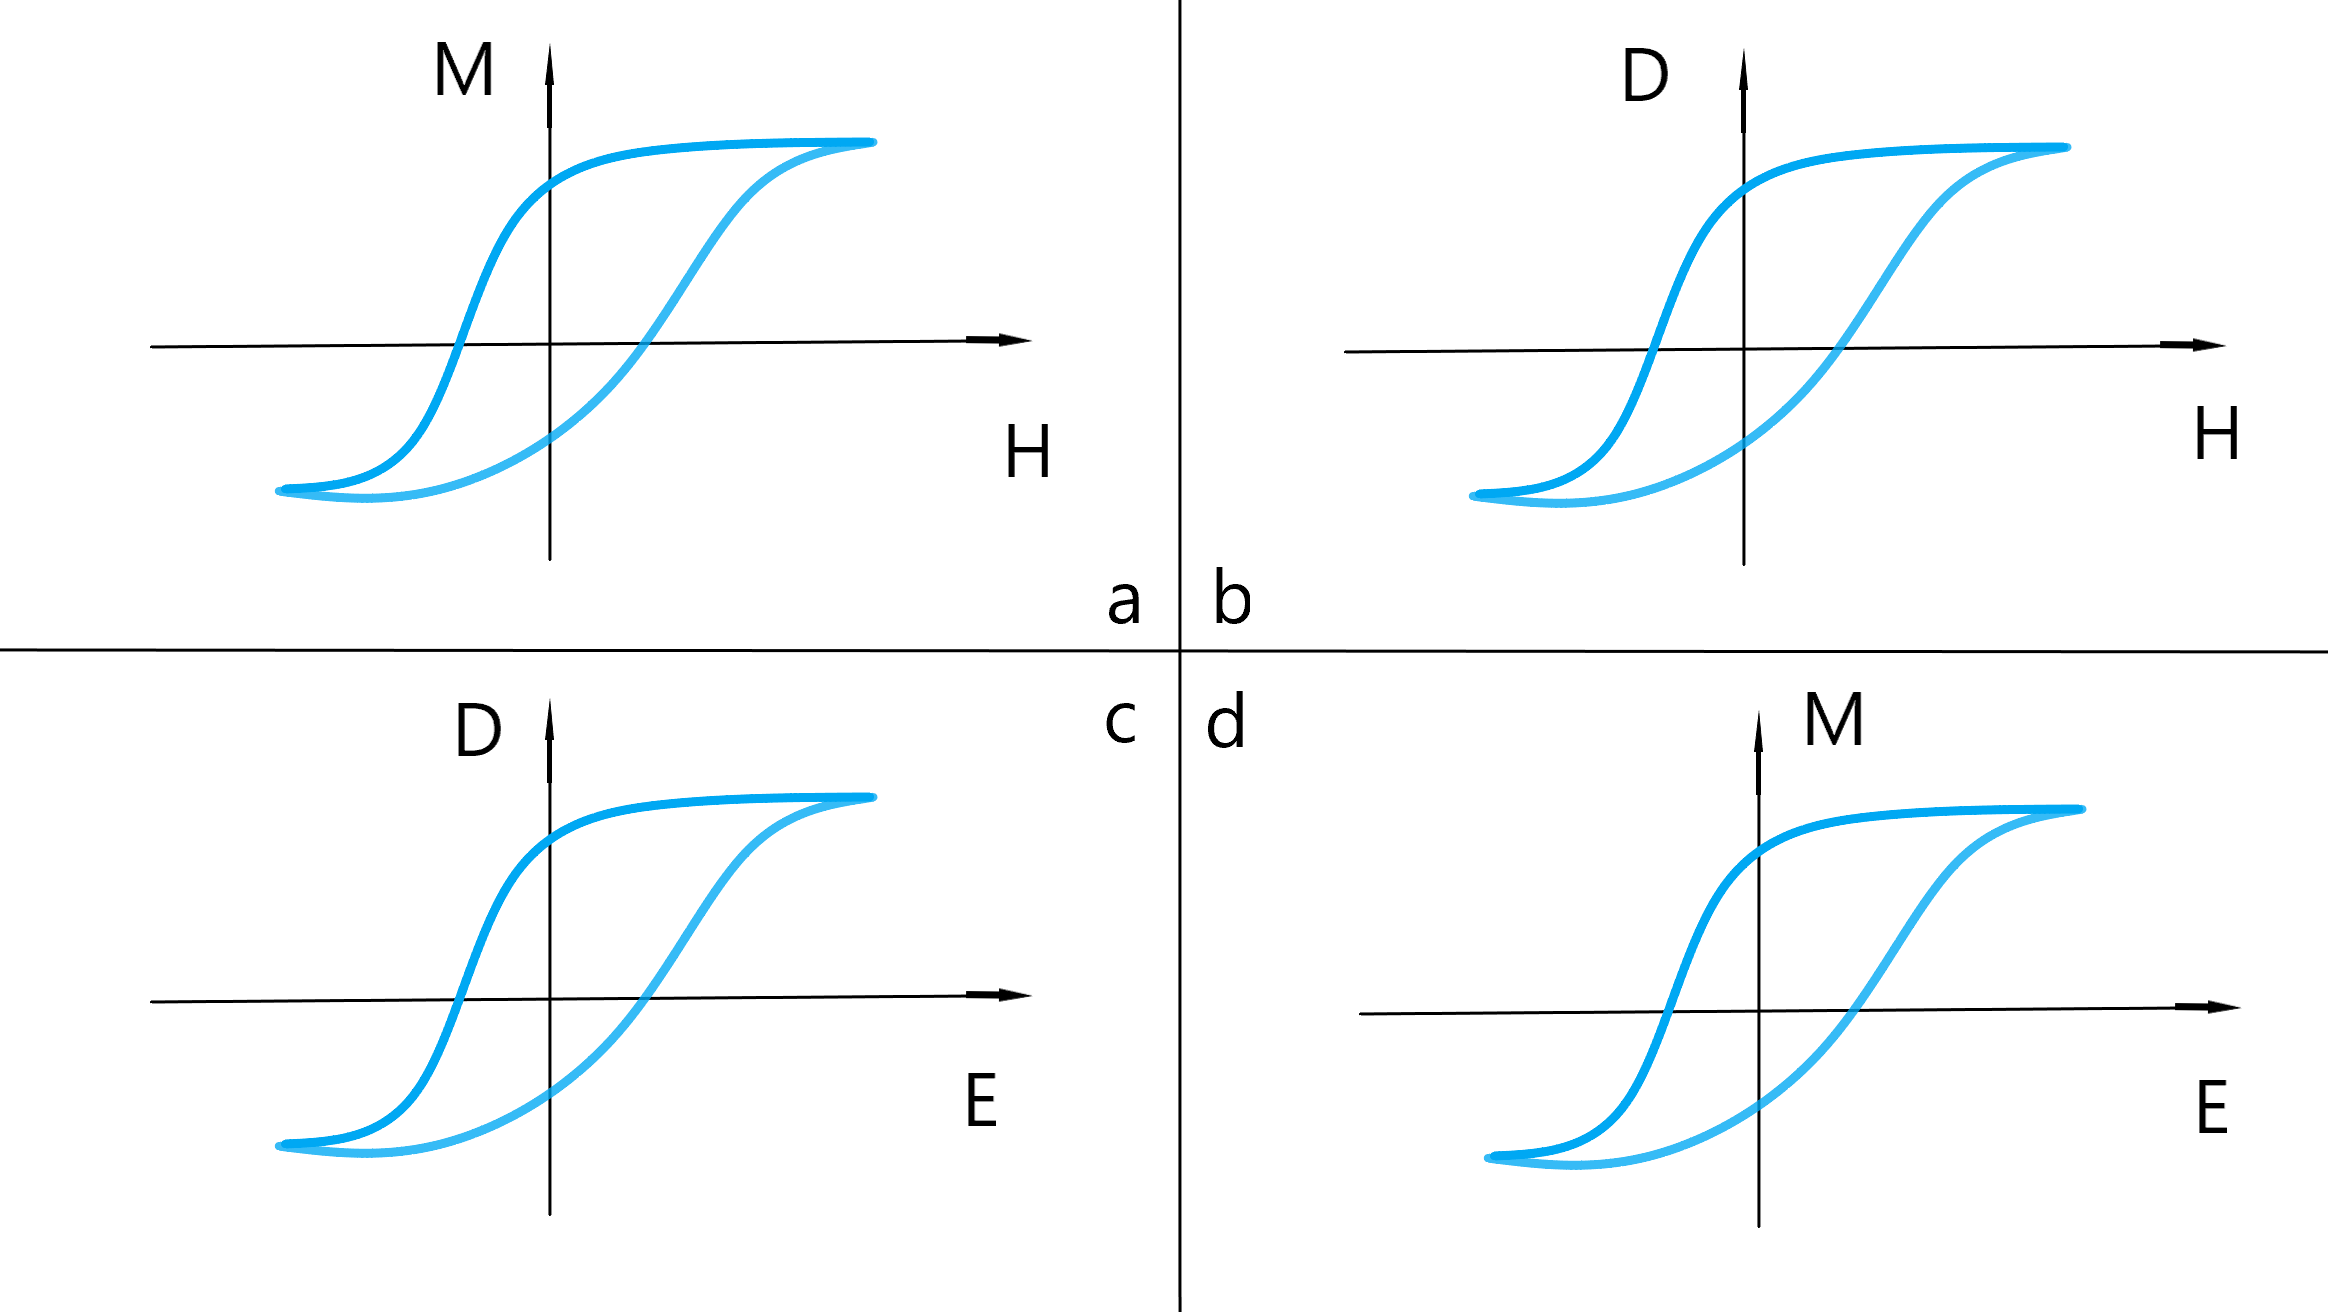
\includegraphics[width=0.8\textwidth]{./pic/003.png}
\caption{铁磁性、铁电性、多铁性示意图  (a)(c)是传统的铁磁性与铁电性,外加磁场可以使铁磁性物质出现磁矩,外加电场会使铁电性物质出现电极化。在外场撤出之后,受外场影响所产生的磁矩与电极化并不会消失。(b)(d)是多铁性材料铁电与铁磁性质的耦合,通过外加电场可以使诱导出宏观磁矩,外加磁场可以产生出电极化。}

\label{dog003}
\end{figure}

\section{多铁材料的基本原理}

多铁材料,一般来说是指同时具有铁电性与铁磁性的材料,结构决定性质,两种性质同时存在必然要求具有能够支撑适应铁电与铁磁的的特殊的微观结构。

\begin{figure}[h]
    \centering
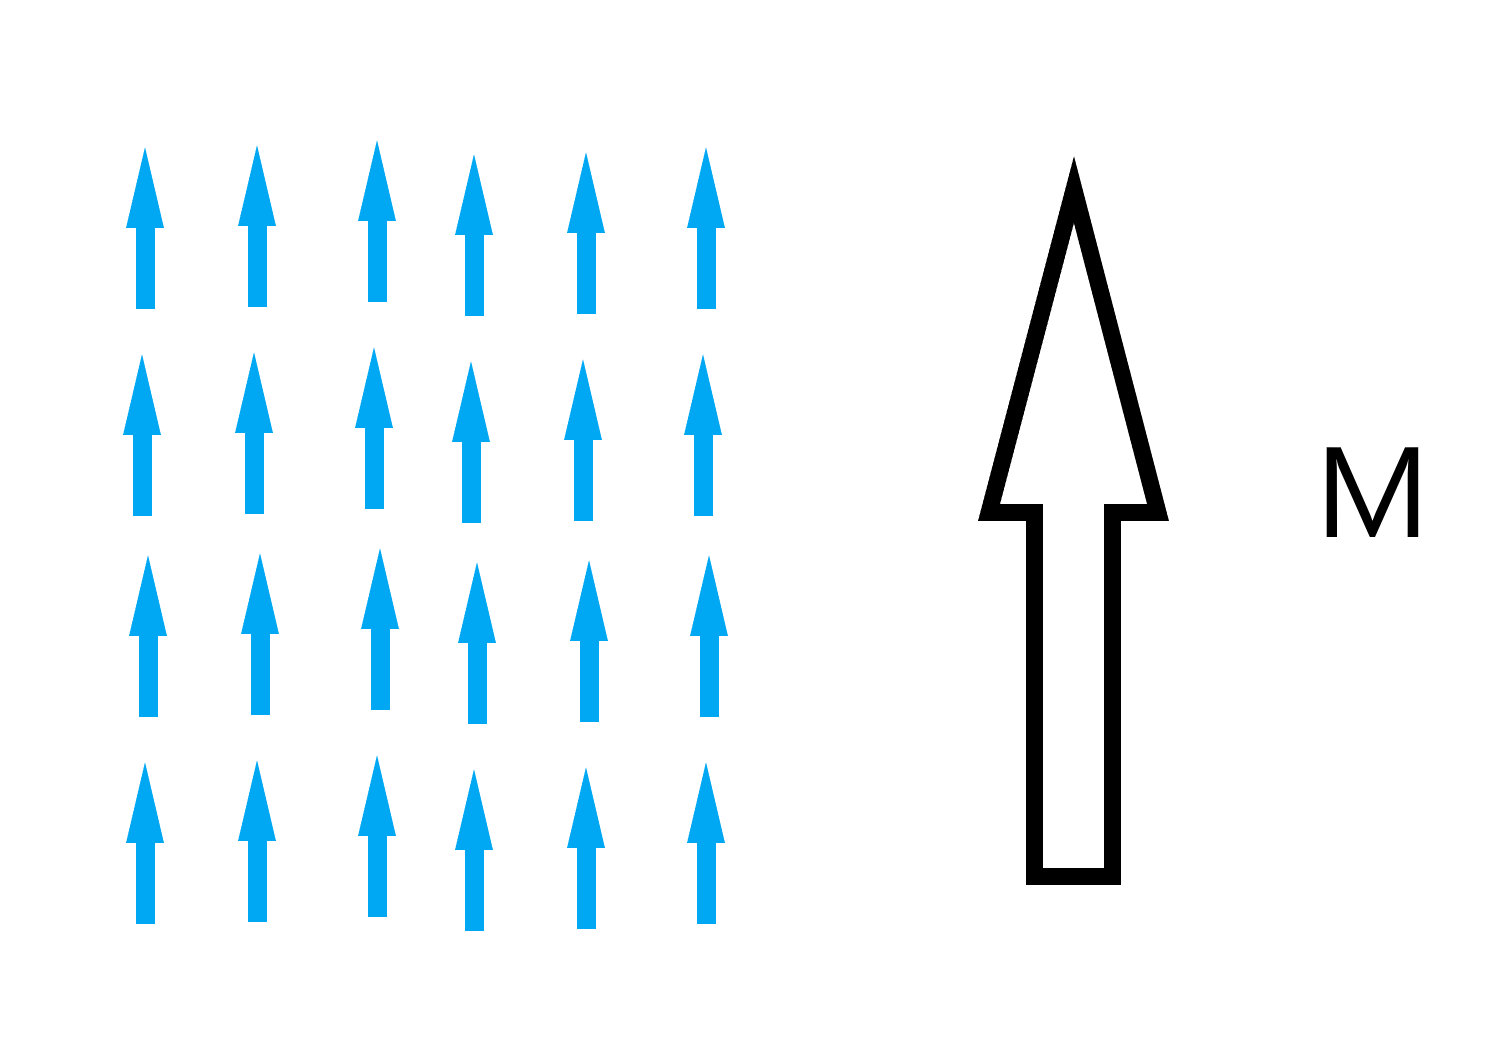
\includegraphics[width=0.8\textwidth]{./pic/001.png}
\caption{铁磁性物质磁化后的微观图像:微观磁矩平行排列,在宏观尺度上表现出磁矩。}
\label{dog001}
\end{figure}

\subsection{铁磁性的来源}

从经典的以麦克斯韦方程组为基础的电磁理论认为,恒定的电流产生恒定的磁场,变化的电流产生变化的磁场。在固体物理领域一般认为,固体的磁性来自电子的轨道运动,电子自身带有自旋、磁矩。固体在宏观上出现磁性微观原因是固体内部的磁有序。从对称性上面看,铁磁性的出现是时间反演对称性的破缺,磁矩产生自电荷的运动,在时间反演下,磁矩会改变方向。经典的看法是,铁磁性材料中的磁矩来源于原子中的未配对电子,通常在d轨道或f轨道电子半满的原子,会产生强的铁磁性。\cite{fiebig2016the} 

\begin{figure}[h]
    \centering
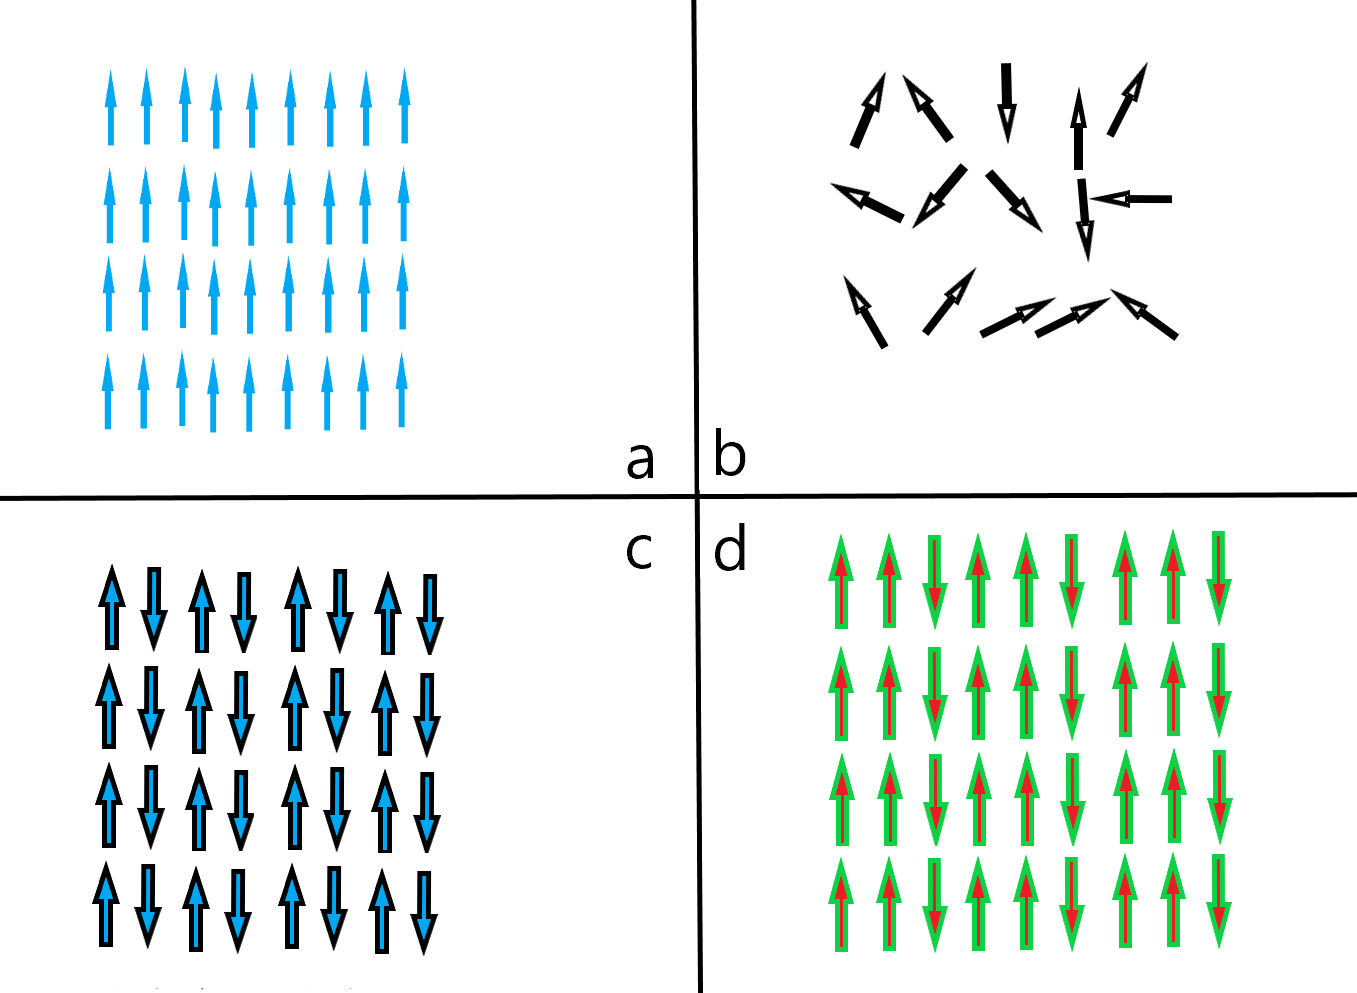
\includegraphics[width=0.8\textwidth]{./pic/002.png}
\caption{铁磁性、反铁磁性、亚铁磁性和顺磁性的微观磁矩图像  (a)是铁磁性物质的微观图像,各个微观磁矩有序排列,微观小磁矩相互叠加,在宏观上表现出宏观磁矩。(b)是具有顺磁性的物质,在无外加磁场的影响下,微观磁矩杂乱无章,随机排列,各个方向磁矩相互抵消,在宏观上不表现出磁矩。(c)是反铁磁性的微观图像,各个微观磁矩有序排列,但方向相反,各处微观磁矩相互抵消,在宏观上不表现磁矩。(d)是亚铁磁性的微观图像,微观磁矩也是规则排列,与反铁磁性不同的是,微观磁矩并没有被完全抵消,在宏观尺度仍然存在磁矩。}

\label{dog002}
\end{figure}

基于元素周期表与核外电子排布规律,传统的铁磁性材料主要来自于过渡金属元素(d电子半充满)与稀土元素(f电子半充满)。\cite{hill2000why}

\subsection{磁有序}

铁磁性的来源与磁有序密切相关,而物质的磁性与微观粒子的内部构造密切相关。磁有序,在宏观上可以产生主要包括铁磁性、反铁磁性、亚铁磁性等材料性质,磁有序的产生与自旋旋转对称性或者时间反演对称的破缺有关。引起磁性的微观粒子的自旋完全是量子力学导出的结果,通过一般经典的理论解释会十分困难,但是,在一定的近似条件或者特定的研究对象的情况下,可以将其视作宏观世界之中的矢量来处理。不同的近似会导出不同的物理模型,常见的描述微观磁现象的模型主要有XY模型、海森堡模型、Ising模型等。\cite{dong2019magnetoelectricity}

\begin{figure}[h]
    \centering
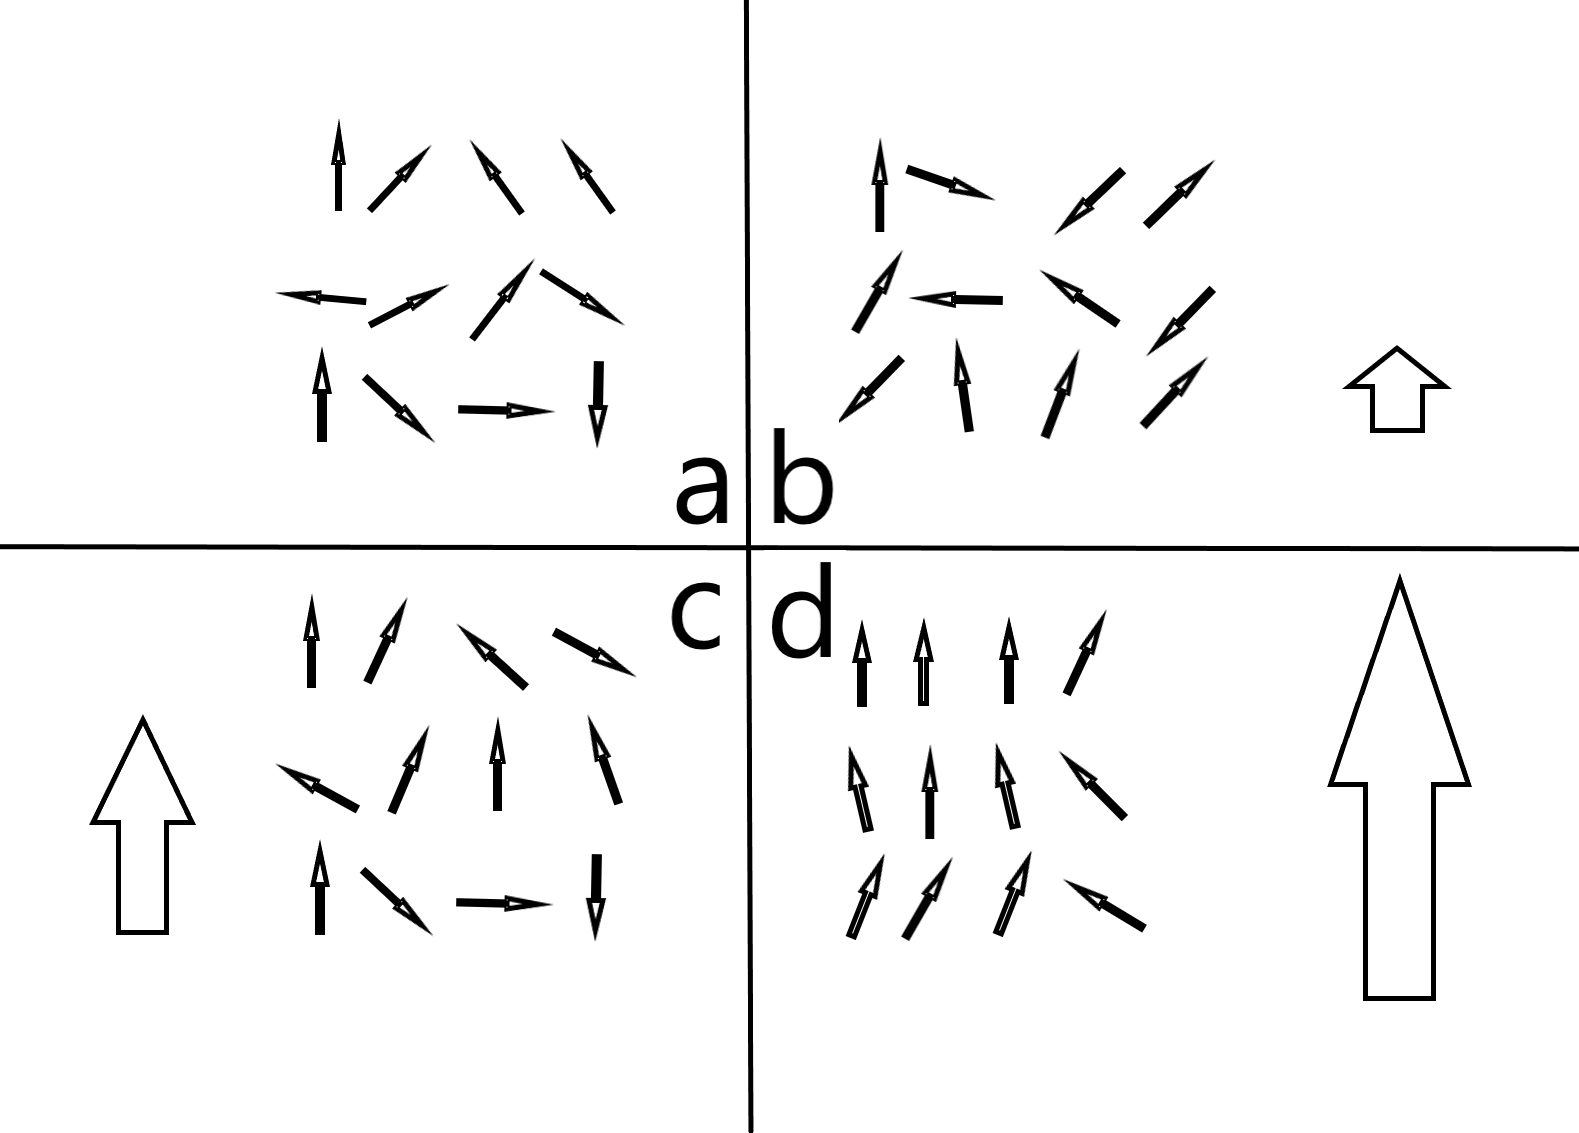
\includegraphics[width=0.8\textwidth]{./pic/005.png}
\caption{顺磁性物质微观磁矩随外场变化\ 图片从(a)到(d)随着外磁场的增加,本来混乱无序排列的微观磁矩会在外加磁场的影响下顺着外加磁场的方向排列,一般来说,外加磁场越强,磁化强度越大。与铁磁性不同的是,当外加磁场去除之后,磁化强度也会随之消失。}

\label{dog005}
\end{figure}

一般材料是由微观层面的原子组成的,原子又是由原子核与核外电子组成的。原子核的磁矩,电子自旋运动的磁矩,电子轨道运动的磁矩三种磁矩构成了原子尺度上的微观磁矩。由于质子、中子等原子核之中的重子比电子质量大三个数量级,原子核的磁矩比电子磁矩小三个数量级,在研究系统自旋磁矩的问题时通常忽略原子核的影响。\cite{王克锋2008单相多铁性材料}在过渡金属元素组成的磁性材料之中,对磁性材料的物理性质起决定性作用的是电子的自旋磁矩。金属材料电子自旋运动的行为可以根据磁化率与的大小与符号划分。
$$\chi =\mathbf{M} /\mathbf{H} $$ 
其中,$\chi$ 为磁化率,$\mathsf{M}$ 是单位体积内部所有磁矩的矢量和,H是外磁场的强度。磁有序行为可以分为五大类行:铁磁性、反铁磁性、亚铁磁性、顺磁性、抗磁性。前三种性质体现出大量磁矩合作的性质,后两种只是磁矩性质的集合。

\begin{figure}[h]
    \centering
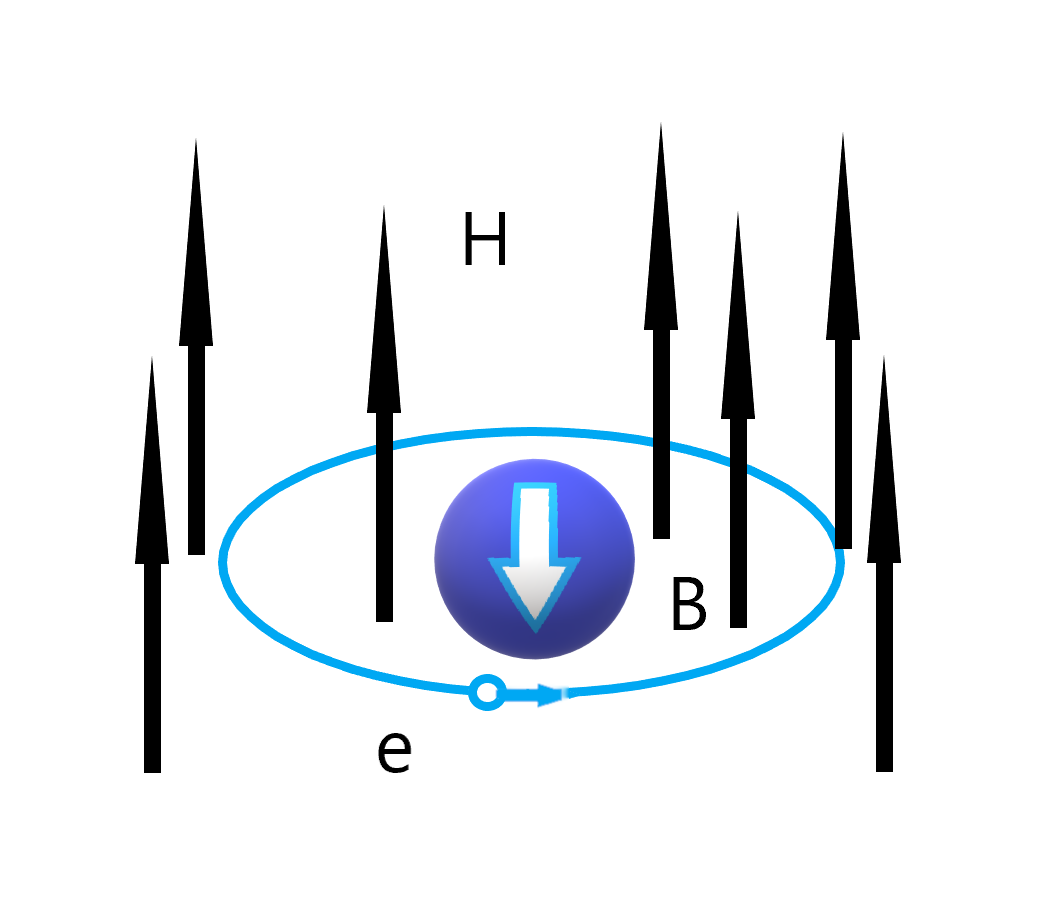
\includegraphics[width=0.8\textwidth]{./pic/004-2.png}
\caption{抗磁性 \ 物质普遍存在的抗磁性是由物质本身微观原子结构决定的。绕原子核运动的电子可以看作一个电流元,在外加磁场的作用下,绕核运动的电子会受到额外的洛伦兹力,这个洛伦兹力会使电子的绕核运动发生改变,依据楞次定律,电子运动改变的结果会削弱外加磁场的影响。}

\label{dog004}
\end{figure}

\paragraph{抗磁性}

实际上,所有的物质(由原子核与核外电子组成的)全部具有或多或少的抗磁性。抗磁性物质具有负的磁化率,一般比较微弱,同时常常被更大的顺磁性的正磁化率所掩盖。抗磁性的微观机理通常很容易解释。根据麦克斯韦方程组以及楞次定律,看作环状电流的电子绕核运动所产生的磁矩在外磁场加入后会因环状电流受外加磁场的影响而变化产生一个抵抗磁通量变化感应磁矩。根据电磁学的一般规律,这种变化是与外磁场方向相反的,普遍存在的抗磁性是经典电磁学“来拒去留”的生动体现,因此其磁化率是负的,而且与温度无关。




\paragraph{顺磁性}
很多固体,如Al、Pd等,具有一定的顺磁性。在顺磁性固体内部的磁矩,分子的无规则热运动会使磁矩无规则取向。外磁场的诱导会使得沿着磁场方向的磁矩数目会有所增加,逆着磁场方向的磁矩数目会有所减少。沿着特定方向磁矩数目的变化会导致产生一个磁化强度M,原来受到热运动影响完全等价的各个空间方向会出现一个特殊取向,即外加磁场的方向,磁矩旋转对称性会被破坏。顺磁性磁化强度是负的,而且与外磁场是线性关系,磁化强度也随外磁场撤离而消失。



\paragraph{铁磁性}
铁、钴、镍是常见的铁磁性材料。铁磁性材料通常有一个转变温度$T_{c}$,低于这个温度的情况下具有铁磁性,高于这个温度的情况下具有顺磁性。这说明在$T_{c}$以下,自旋有自发平行的取向,当温度提高之后自旋取向无规律,在$T_{c}$以上铁磁性物质的磁性行为与顺磁性物质类似,磁化率与温度关系满足居里定律。

\paragraph{反铁磁性}
常见的反铁磁性材料有铬和锰,与铁磁性物质一样反铁磁性也有一个转变温度,在转变温度以上时具有顺磁性性质,在转变温度$T_{N}$以下时,一半自旋与另一半自旋是反平行的,总磁化强度为0。

\paragraph{亚铁磁性}
铁氧体如$Fe_{3}O_{4}$是常见的亚铁磁体,与反铁磁性物质相似,在$T_{c}$以上微观磁矩无规则排列,在$T_{c}$以下,微观自旋按照反平行排列。不同的是,反平行排列的微观磁矩大小不相等,因此在宏观上是存在磁矩的。亚铁磁性物质另一个特点是在转变温度以上很大温度范围内并不遵守磁化强度与温度相关的居里定律。

这几种磁有序性质之中,最有趣最重要、应用最广的是铁磁性,尤其是其在外加磁场撤除之后的磁滞回线。这几种磁有序虽然在性质特点与磁性行为上各有不同,但在本质上是有共同点的,是同一种物理规则支配下的不同表现形式,磁有序结构归根究底是晶格上的离子磁矩以及离域电子磁矩的直接或间接的相互作用。

\begin{figure}[h]
    \centering
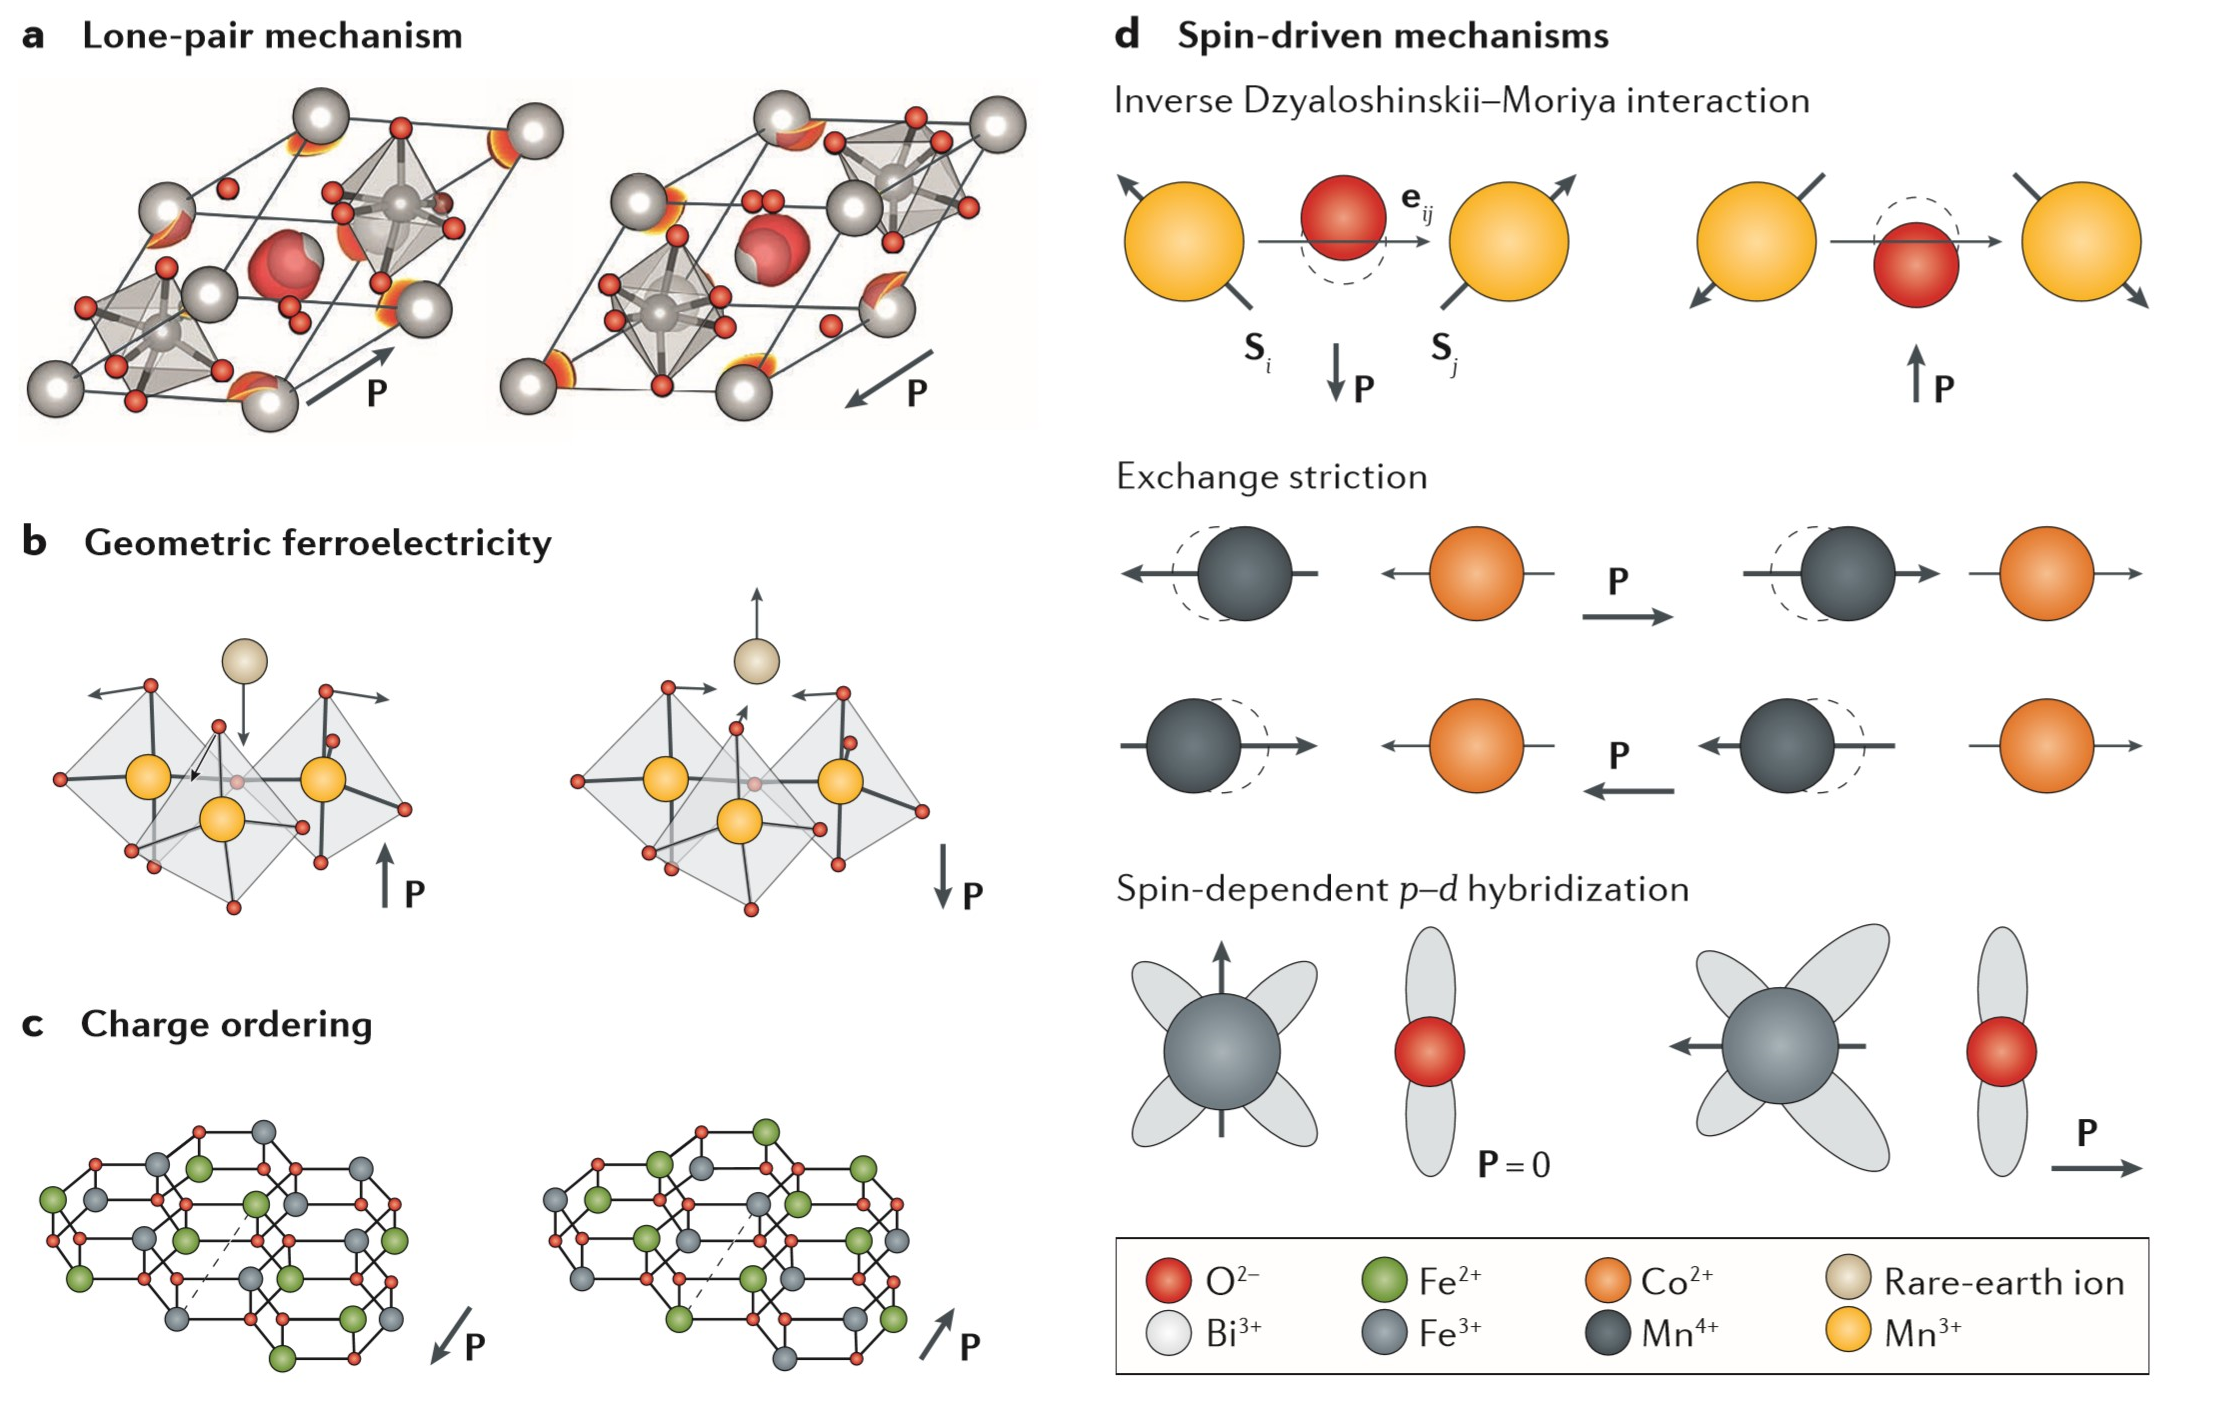
\includegraphics[width=0.8\textwidth]{./pic/006.png}
\caption{多铁材料铁电性的来源机制}
\small
(a)孤对电子机制。典型存在于$BiFeO_{3}$,$Bi^{3+}$离子中的两个电子偏离Bi趋向与氧铁八面体,使晶体内部正负电荷中心偏离,产生了电极化强度。(b)几何机制。典型是$RMnO_{3}$,稀土元素氧离子收到晶格之中氧八面体的几何限制,会在某些方向上面产生电极化。(c)$LuFe_{2}O_{3}$之中的电荷排序。在层状结构之中不同层内$Fe^{3+}$和$Fe^{3+}$的比例不同,这会形成一个电极化。(d)其他的有自旋引起的电极化。主要有Dzyaloshinskii–Moriya作用、交换作用、自旋依赖的p-d轨道杂化等复杂的量子力学相互作用。

\label{dog006}
\end{figure}

\subsection{位形空间中的磁结构}

在实验方面,通过中子衍射可以测量出磁矩在晶格之中的分布,氧化物绝缘体的磁性现象很容易从晶格结构与自旋分布方面解释。例如MnO,其晶体结构与NaCl类似,阴阳离子交替排列。带有自旋磁矩$Mn^{2+}$交替反平行排列,在宏观上没有净磁矩,是典型的反铁磁性。铁氧体是典型的亚铁磁性物质,在$Fe_{3}O_{4}$内部,氧离子按照类似面心立方最密堆积进行排列,金属阳离子只能占据四面体空隙与八面体空隙。在铁氧体内部,按照1:2比例存在着二价铁离子与三价铁离子。通过实验证明,三价铁离子按照1:1的比例填充在八面体与四面体空隙之中,二价铁离子全部填充在八面体空隙之中。八面体空隙之中的自旋与四面体空隙中的阳离子方向反平行。三价铁离子对系统磁矩的贡献相抵消,宏观磁矩实际上是二价铁离子提供的。

\subsection{波矢空间中的磁结构}

在实空间中磁有序可以看做磁矩在周期性格点上的规律排布。磁结构的来源与自旋电子密切相关,在倒格空间之中也可以显示磁现象的能带结构。基于自旋密度泛函的计算结果,可以提供不同自旋取向的磁能带态密度随能量分布曲线。非磁性固体的磁能带是完全对称的,而铁磁性固体有着明显的不对称。不对称导致了不同自旋取向的电子数目不同$N_{\uparrow }\neq N_{\downarrow }$,从而产生自旋极化,可以用来解释金属具有铁磁性的物理起源。


\subsection{铁电性的来源}

铁电性的根源是电极化,通常认为,铁电性来自微观结构之中的电偶极矩,电偶极矩的本质是空间之中的正负电荷中心的不重合。微观结构上空间中的正负电荷有序排列,在宏观就观察到铁电性。从对称性上来看,铁电性的出现是空间反演对称性的破缺。一般来说铁磁性与自发极化需要空的d轨道与孤对电子。

若要获得同时具备铁电性与铁磁性的则需要同时具备以上两种的形式,既要有磁矩又要有电矩,既要有时间反演对称性的破缺又要有空间反演对称性的破缺。

\subsection{多铁材料中的电磁耦合}

单独的铁磁性与铁电性在普通材料之中比较常见,对多铁材料,研究其铁磁性与铁电性的耦合机制有着重要的作用。作为电子自身固有运动的两个属性,电荷与自旋从根本上衍生出电偶极矩与磁矩与铁电性和铁磁性密切相关。研究多铁材料之中铁磁性与铁电性,电荷空间分布与自旋的联系对解开多铁材料的秘密与设计制备新型高性能多铁材料有着重大的理论价值与实践意义。通常认为,多铁材料之中的电磁耦合有三个来源:自旋轨道耦合、自旋晶格耦合与自旋电荷耦合。\cite{nan2019multiferroics}

\paragraph{自旋轨道耦合}
自旋轨道耦合是一种典型的相对论量子力学的结论与效应。运动的电荷产生磁矩,铁磁性的产生与时间反演对称密切相关,电偶极矩的产生与正负电子在空间的分布有关,铁电性的产生与空间电子分布对称性有关。目前看来,能同时联系时间与空间的只有相对论理论,所以解释多铁材料之中电磁耦合的原理应该有来自相对论量子力学的部分。从半经典的角度来看,电子自旋产生磁矩,电子绕核的轨道运动会导致电子在空间中机率密度分布不均衡,特定的轨道运动形式会导致空间对称性的破坏。在一些特殊材料中(例如$TbMnO_{4}$),特殊的磁结构会导致空间反演对称性破话,而自旋轨道耦合会将这种对称性破缺转化为空间中的电偶极矩。相反的如果空间对称性被破坏,自旋轨道耦合也会对磁矩有影响。

\paragraph{自旋晶格耦合}
磁性离子之间的磁相互作用,无论是常规的对称交换作用还是反对称的DM作用,都是取决于电子交换路径的细节。从微观分子角度上看,化学键成键的键长与夹角的改变会对波函数的重叠有影响,进而会影响交换作用。\cite{moriya1960anisotropic}
宏观上的磁致伸缩效应是指在材料在磁场下或者磁化后,宏观上的尺寸会发生变化。压电铁电材料之中的自发极化也会受到晶格畸变的影响,铁磁与铁电性质可以通过晶格结构的改变间接耦合。

\paragraph{自旋电荷耦合}
自旋电荷耦合是由电子密度分布决定的。在磁性系统中,载流子(电子、空穴)可以被自旋极化,因此局域的磁矩可以被电荷密度分布调控,外电场、磁场都可以成为驱动载流子运动的动力。

通常来说,多铁材料内部铁电性与铁磁性耦合很少是由单一原因造成的,通常情况下是由一种原因占主导地位,其余方面处于次要地位。

\subsection{多铁材料的分类}

多铁材料要求同时具有铁电与铁磁两种性质,可以通过两种性质的来源是否相同将多铁材料费为两类,第一类是铁电铁磁两种性质的来源不同,即两种各自独立发挥作用。例如最著名的多铁材料$BiFeO_{3}$\cite{姚携菲2014磁电多铁性材料的宠儿},其中$Bi^{3+}$提供孤对电子,在晶体结构内部产生一个电偶极矩,三价铁离子提供磁矩。两种因素相互配合,使其在宏观上同时表现出铁电性与铁磁性。第二类多铁材料是指材料的铁磁性与铁电性是同源的。\cite{段纯刚2009磁电效应研究进展} 多铁材料可以根据多铁性的具体来源可以进行进一步的细分。



\paragraph{复合多铁材料}
这种多铁材料的产生原理并不复杂,把一种只有铁电性的材料,例如$BaTiO_{3}$与一种只有铁磁性的材料,如$CoFe_{2}O_{4}$混合起来,一层一层叠加在一起,层层生长形成超晶格,在室温下实现了磁场与电场的耦合,并可以通过控制磁场的方式影响电极化。其优点是耦合强度高,在室温下稳定存在。但这样层叠复合材料就不是单相材料了,另外,利用电场控制磁场的效应仍待进一步研究。\cite{vaz2010magnetoelectric}

\paragraph{孤对电子机制}
这种多铁材料是单相的,一般包含两种及以上的阳离子,一种提供孤对电子与铁电性质,另一种提供磁铁性。上文提到的$BiFeO_{3}$就属于这一种。$BiFeO_{3}$是一种在室温下,具有强电磁耦合的,稳定的电极化的单相多铁材料。

铁酸铋是多铁材料之中比较重要的一个,经过数十年的发展,进行过大量的研究。铁酸铋的铁电极化与磁有序的耦合在室温以上的温度下依然存在。$BiFeO_{3}$蕴含着大量的新物理与潜在应用,其内部存在的T型结构与R型结构仍待研究,其独特的光电效应光催化、光摩擦、光变色、气体敏感、表面现象是研究的热点。\cite{姚携菲2014磁电多铁性材料的宠儿} 

\paragraph{几何驱动的铁电性}
这种材料的铁电性的来源是几何性质的因素。某些几何学上的限制会导致结构不稳定,从而使某些离子位移,进而产生电偶极矩。例如一个小的阳离子可以允许周围的配位多面体旋转,这些配位多面体本身带有极性。这类材料的代表是$BaNiF_{4}$,这些新开发的材料在铁电性上都不如传统铁电材料,主要的阶数参数是转动阶数,而不是铁电极性畸变。改良这类材料的关键是对铁电性的具体机制进行研究。\cite{fox1977ferroelectrically} 

\begin{figure}[h]
    \centering
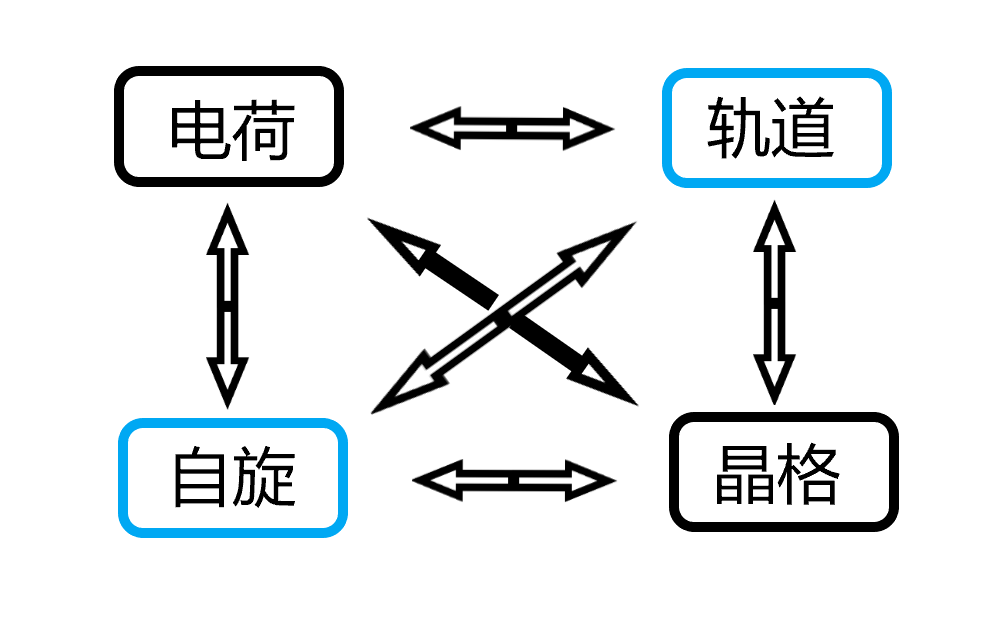
\includegraphics[width=0.8\textwidth]{./pic/008.png}
\caption{多铁材料中的电磁耦合}

\label{dog008}
\end{figure}

\paragraph{电荷排序} 
价电子在主要离子周围的分布可能是不均匀不对称的,这在晶体结构上可能会产生一个电偶极矩。主要的例子是$LuFe_{2}O_{4}$,其内部的三价铁离子与二价铁离子在不同层间的比例不同,不仅破坏了空间反演,这导致了电荷在空间的有序排列以及层间的电偶极矩。\cite{qin2015an}

\paragraph{自旋驱动的铁电性}
这类多铁材料是一种铁电铁磁同源的多铁材料,电子自旋不仅引起了铁磁性,而且还产生了电极化。目前认为自旋引起的极化可能有三种来源:DM(Dzyaloshinskii–Moriya)相互作用\cite{dzyaloshinsky1958thermodynamic}、类海森堡的交换作用、依赖自旋的轨道杂化。铁电铁磁同源的铁电材料的电磁耦合强度是最高的。
\chapter{二维多铁材料}

\section{二维材料}

二维材料有很多种一般并不存在于自然界中,绝大部分二维材料是人工合成或制造的,自从石墨烯被发现之后,二维材料以其多种多样的性质受到人们的广泛关注。以二维材料为代表低维材料在一个或多个维度上空间尺度与微观粒子尺度相近似,支配微观世界的量子力学等微观规则与性质会在宏观尺度上表现出来,研究低维材料对解决基础理论或实际应用上面重大问题有很大帮助。\cite{novoselov2004electric}随着对铁磁、铁电和多铁材料的进一步研究,对新物理、新材料的研究使研究对象由高维(三维)向低维扩展。

多年以来,对常规的三维多铁材料的研究有很多进展,但至今没有一种广泛应用的在室温下稳定的多铁材料进入应用领域。另一方面,由于二维材料在一个方向上有着与微观粒子相同的尺度,二维材料常常有着与常见的三维材料截然不同的性质与现象,二维材料可能在自发极化强度、电磁耦合强度等各种基本性质上与三维材料有着显著差异。对多铁性来说,材料的降维会是对称性元素减少,有利于铁电性、铁磁性等对称性破缺等性质的产生。另外二维材料巨大的比表面积使其更容易受到外在环境变化的影响,采用外加电磁场、进行原子、分子、离子吸附掺杂等方法进而改良物理性质变得更加容易。然而,受制于二维材料不稳定的先天缺陷,低成本、稳定的、可实用二维材料的寻找、制备、应用的过程会比常见的三维材料更加困难。

\section{二维材料的磁性质}
二维材料不仅拥有很多新的电子学性质,还拥有很多新奇的磁学性质。同非二维材料一样,二维材料的磁性是来源于电子轨道之中的未配对电子。由泡利不相容原理以及洪特规则可得,最先填充一个电子壳层的若干电子自旋方向倾向于相同,这些电子将优先占据能量较低多数多数自旋态而使局域原子显出磁矩。局域磁矩按照一定规律排列组合,即可在宏观尺度上表现出磁性。二维磁性材料像三维磁性材料一样,也可以分为铁磁性、亚铁磁性、反铁磁性、顺磁性、抗磁性。铁磁性二维材料具有自发极化磁矩,在外场作用下可以实现磁矩方向的翻转,在外场撤出后仍然保留比较大的剩余磁化强度,有着广泛的应用前景与研究价值。

目前发现的二维材料大多不具备铁磁性,二维材料之中产生铁磁性的重要一点是在二维材料内部产生未配对电子,进一步使二维材料的电子态密度产生自旋劈裂,即不同自旋方向的电子态密度出现不对称。从二维材料的能带结构上面看来,二维铁磁材料可以分为三种:铁磁半导体、铁磁导体、铁磁金属。铁磁半导体在发生自旋能级分裂时没有被费米面穿过,与半导体一样存在带隙。铁磁导体中发生自旋分裂的两种自旋方向能级被费米面穿过,没有带隙。铁磁半金属有一个自旋方向的态密度被费米面穿过,没有带隙,另一个自旋方向没有被穿过,存在带隙保持着绝缘体或者半导体的性质,对一个自旋方向的电子来说是导体,对另一种自旋方向的电子来说是绝缘体,这种半金属半绝缘体的性质可以用来选择性过滤某种自旋方向的电子。为增强铁磁性,通常在二维材料之中,一般采取载流子掺杂的方式,提高费米面附近电子密度,进而引发电子自旋分裂产生铁磁性。

\begin{figure}[h]
    \centering
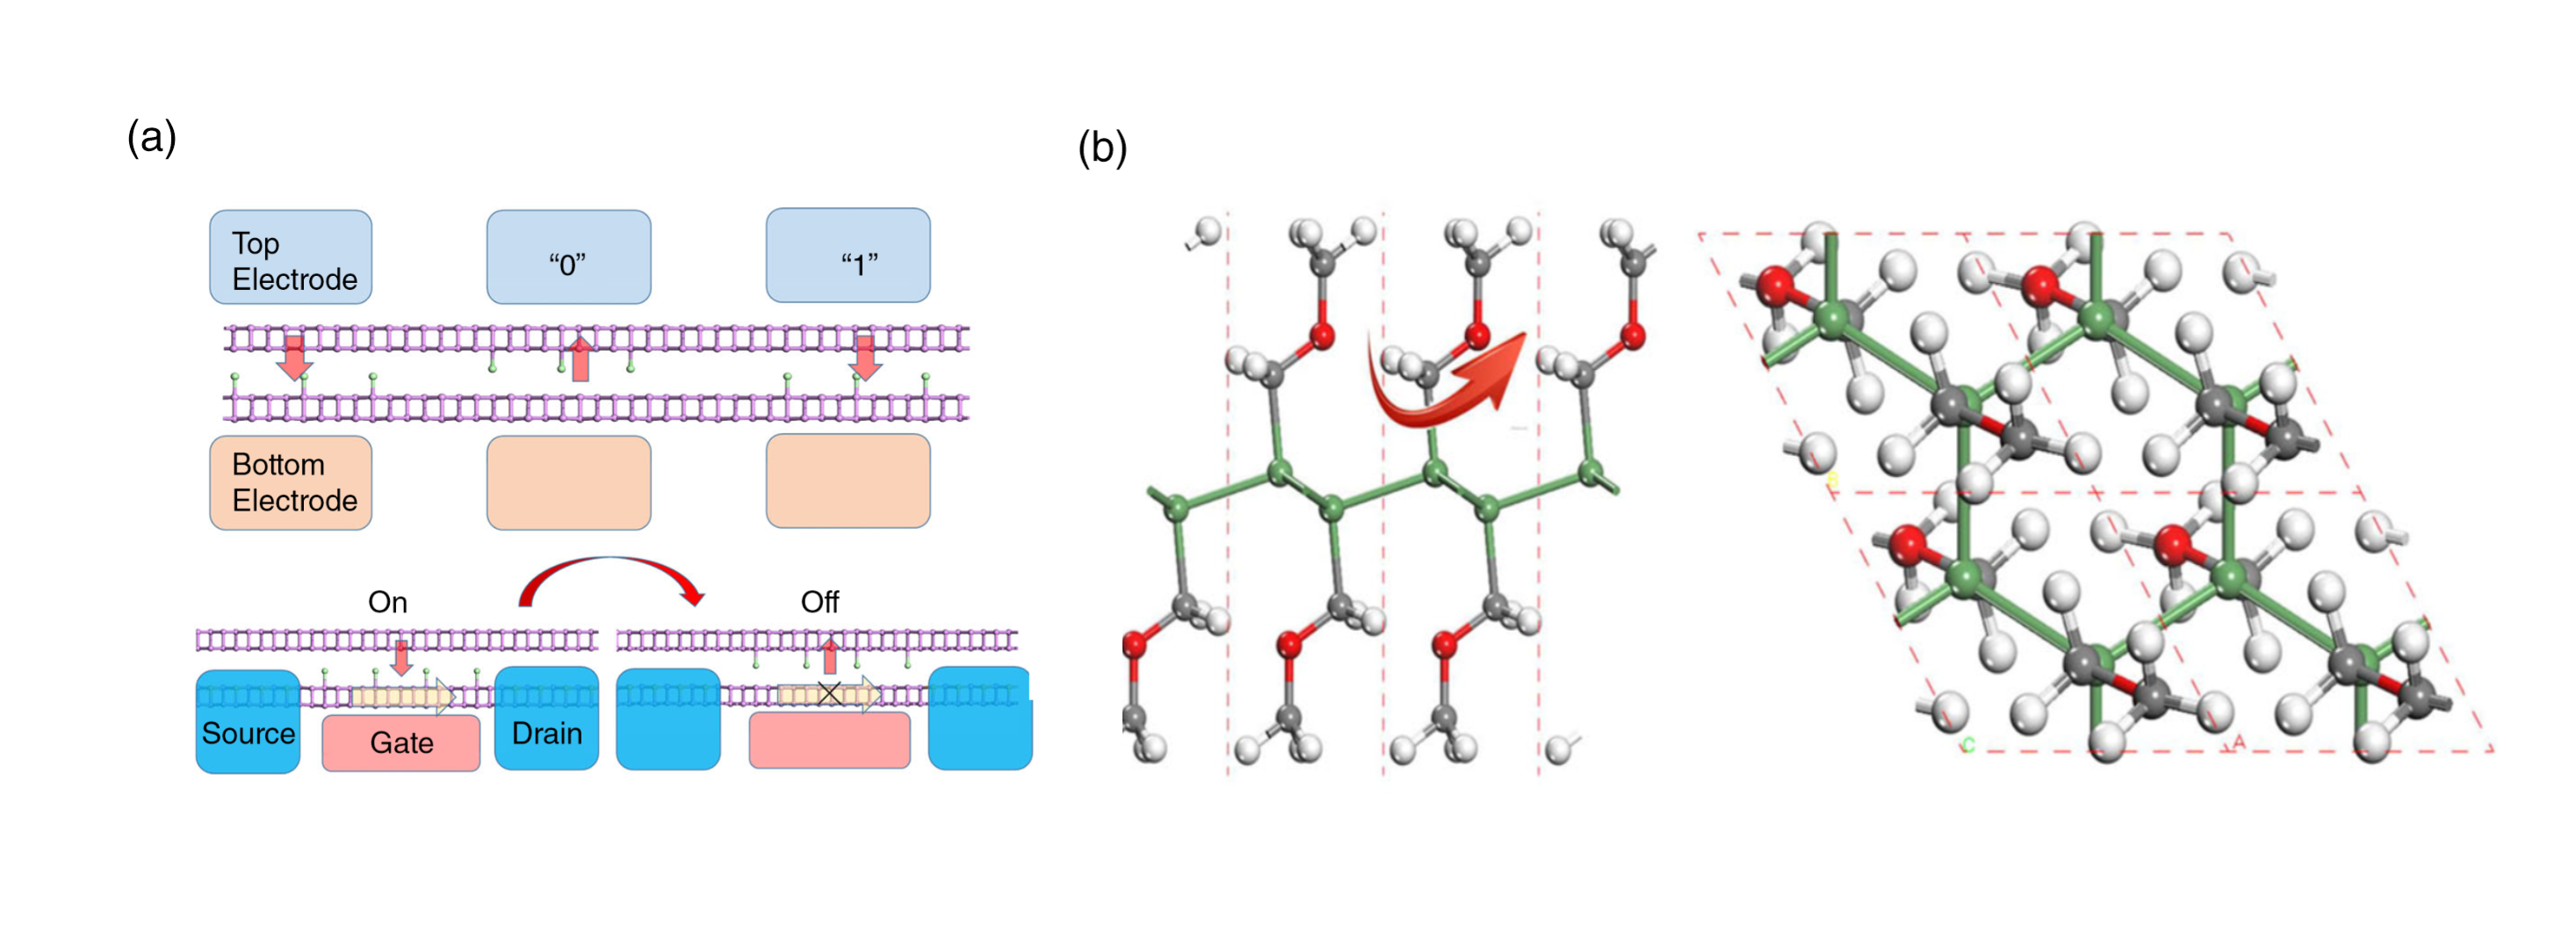
\includegraphics[width=0.8\textwidth]{./pic/015.png}
\caption{(a)卤素原子在磷烯双层之间的迁移形成垂直二维平面的电极化,通过外加电场使卤素原子在两层间的迁移实现电极化的反转,可以用来制作磁读电写存储器与多铁场效应管 \ (b)添加$CH_{2}OCH_{3}-$后的锗烯层,通过添加后的极性官能团在平面内的旋转实现电极化方向的转换}

\label{dog015}
\end{figure}

\section{二维材料的铁电性}

与三维材料一样,铁电性是由自发极化的电偶极矩形成的,微观层面的正负电荷中心不重合产生的电偶极矩,按照一定的规律组合叠加起来,最终形成宏观的电偶极矩。目前发现的具有铁电性的二维材料比较少,主要来源于中心对称缺失的二维晶体结构。

\begin{table}[!htbp]
    \caption{常见的二维铁电材料}
    \label{tab:dog}
    \resizebox{\textwidth}{!}{
    \begin{tabular}{lllllc}
        \toprule
        
        材料 & 极化强度(pC/m) & 电极化方向 & FE switch barrier(meV/f.u.) & 转变温度(K) &参考资料 \\
        \midrule
        1T-$MoS_{2}$ & 0.28 $μC/cm^{2}$ & 垂直平面 & 未见报道 & 未见报道 & \cite{shirodkar2014emergence} \\
        Group IV binary AB, Group III–V binary AB & 0.88–4.22, 7.82–11.45O&垂直平面&160–390, 50–300&未见报道&\cite{di2015emergence}\\
        SnS, SnSe, GeS, GeSe&151–506&面内&3.76–580.77&326–6400&   \cite{fei2016ferroelectricity}\\
        $\beta -GeSe$&160&面内&5.83&200&\cite{guan2018tunable}\\

        As, Sb, Bi&46–151&面内&5.83–183.6&463–680&\cite{xiao2018elemental}\\
        SnTe&未见报道&面内&未见报道&270&\cite{chang2016discovery}\\
        GeTe&32.8$μC/cm^{2}$&面内&37.4&570&\cite{wan2017promising}\\
        $\alpha -In_{2}Se_{3}$&2.36e Å, 0.11e Å&面内,垂直平面&57T&室温&\cite{ding2017prediction}\cite{zhou2017out}\cite{cui2018intercorrelated}\\
        $\beta -In2Se3$&未见报道&面内&未见报道&473&\cite{zheng2018room}\\
        $WTe_{2}$&~0.16&垂直平面&未见报道&350&\cite{fei2018ferroelectric}\\
        $CuInP_{2}S_{6}$&未见报道&垂直平面&未见报道&320&\cite{liu2016room}\\
        $AgBiP_{2}Se_{6}$&1.2&垂直平面&6.2&超过室温& \cite{xu2017monolayer}\\
        $CuInP_{2}Se_{6}$&0.322$μC/cm^{2}$&垂直平面&80&150&\cite{song2017off}\\
        Graphene-OH&6.6$μC/cm^{2}$&面内&未见报道&700&\cite{kan2013high}\\
        Ge, Si, SnSb, $MoS_{2}$−SAM&31–117&面内&~90 per ligand&超过350&\cite{wu2016ferroelectricity}\\
        Sc2CO2&176, 1.60μC/cm2&面内,垂直平面&520&超过室温&   \cite{chandrasekaran2017ferroelectricity}\\

        \bottomrule
    \end{tabular}}
\end{table}


\subsection{固有极化的二维铁电材料}

通常来说,铁电材料在居里温度以下会产生自发极化,外加电场很容易影响这种自发极化的大小与方向。二维材料产生自发极化,必然有着一个使系统对称性降低极化方向,一个与众不同的特殊方向方向。到目前为止,有一部分二维铁电材料被发现。这些材料的组成元素具有多样性,自发极化的方向有平面内的和垂直于二维平面的,其性质也各不相同。

\begin{figure}[h]
    \centering
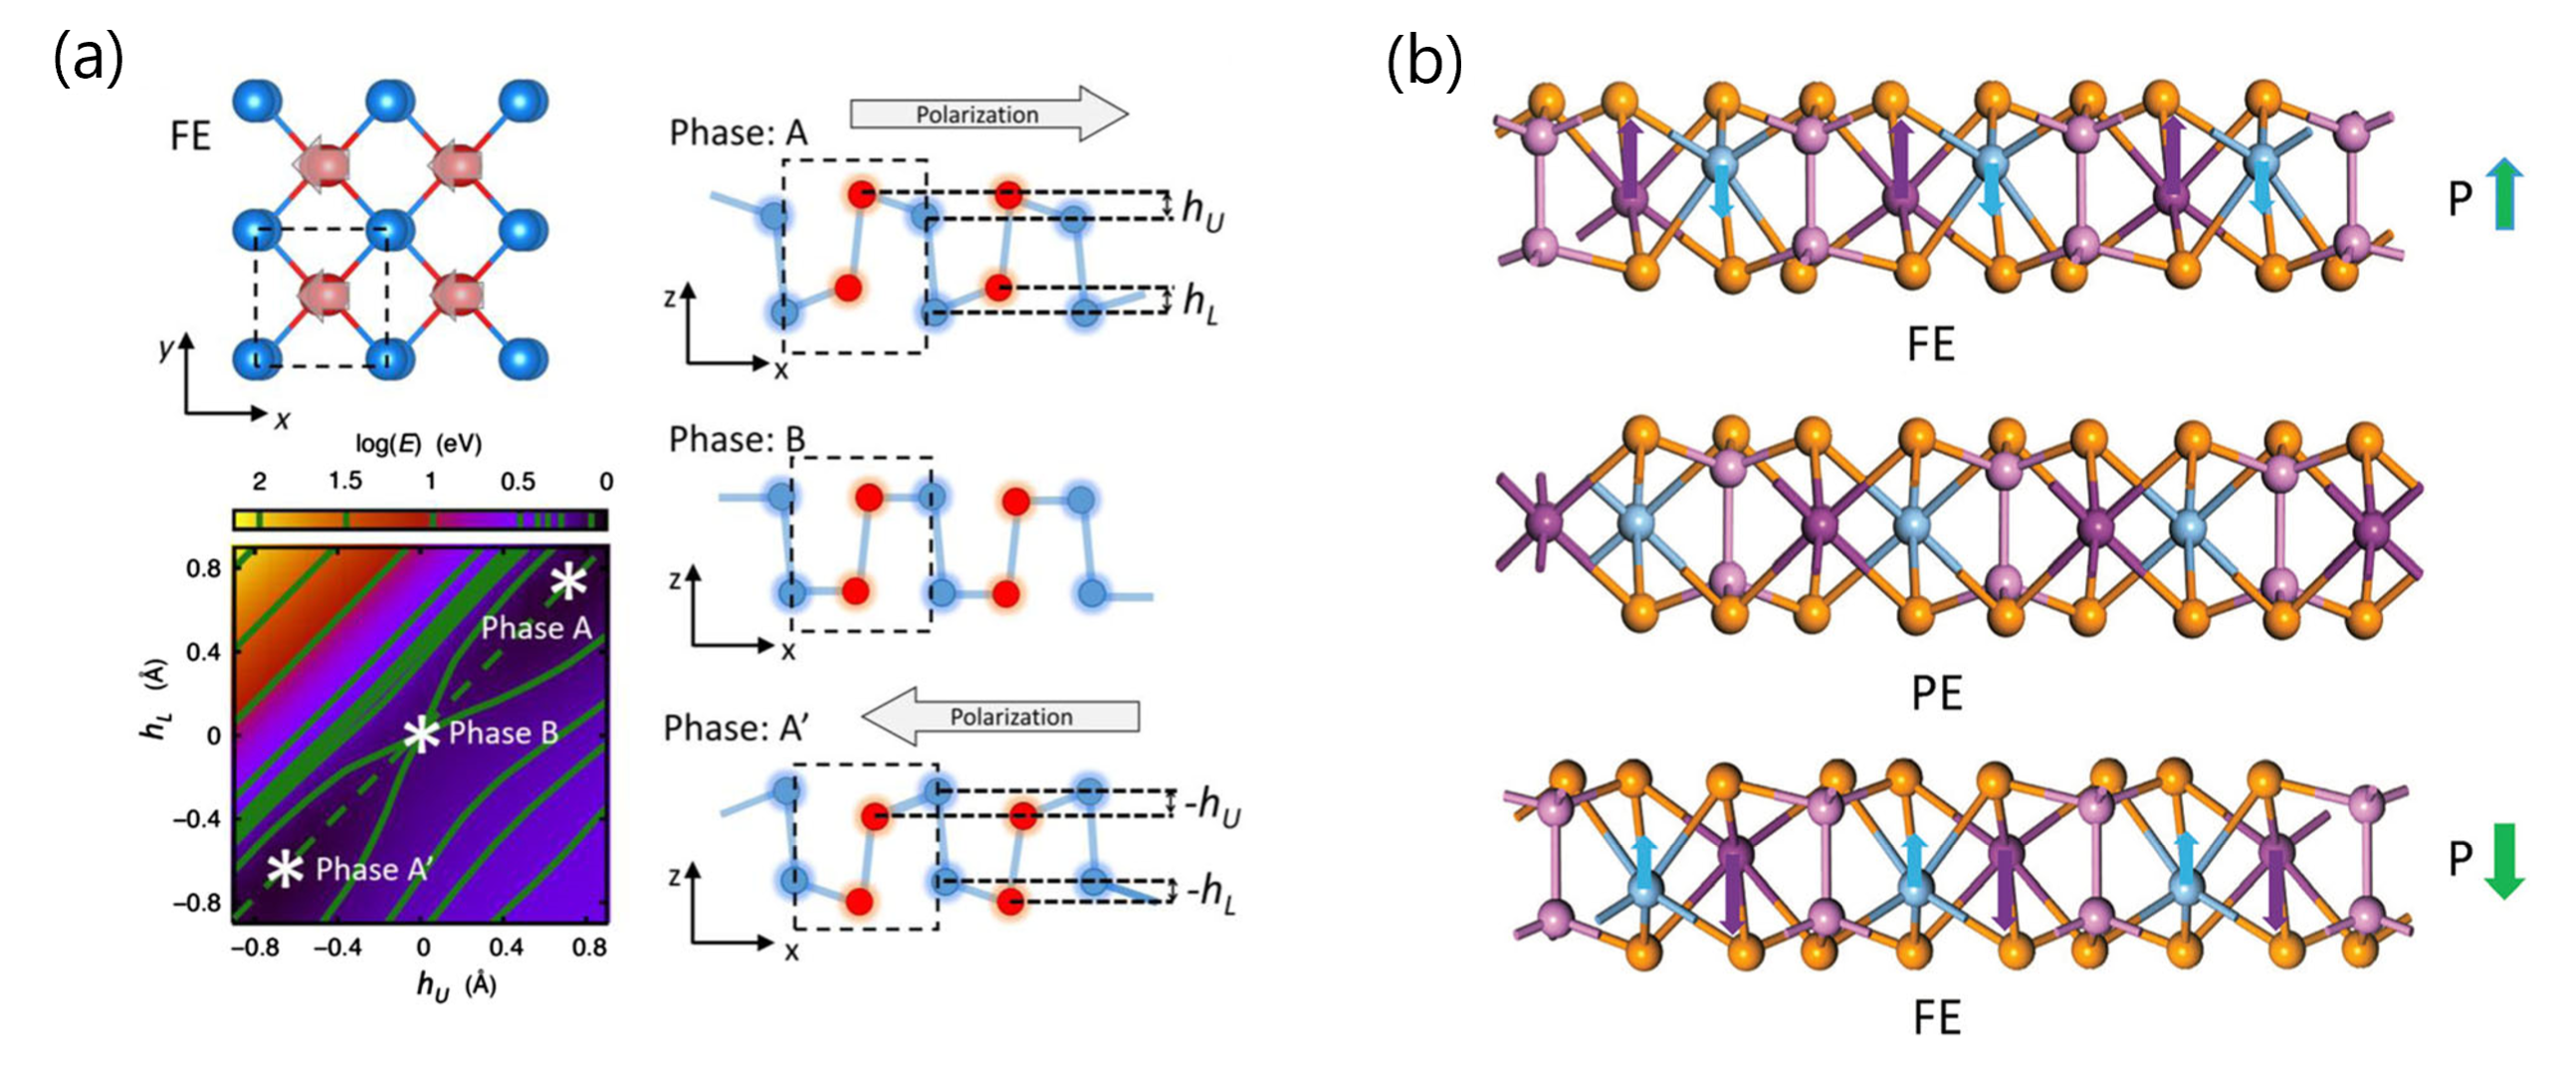
\includegraphics[width=0.8\textwidth]{./pic/016.png}
\caption{(a)第五主族元素形成的二维铁电材料,晶格不同的畸变扭曲方式形成了三个相,其中两个不对称的铁电相,一个对称的没有电极化的相(b)复杂组分的二维铁电材料通过离子不同的位移形成电极化}

\label{dog016}
\end{figure}

$MoS_{2}$ 是一种在垂直二维平面产生极化的二维铁电材料,其单层结构的垂直极化大约可达$0.28μC/cm^{2}$。在第四主族元素或者第三到第五主族元素形成的二元二维膜中也发现过二维铁电材料,例如$SiGe\text{、}SiSn\text{、}GeSn\text{、}AlSb\text{、}GaP\text{、}GaAs\text{、}InP\text{、}InAs\text{、}InSb$等。以上这两种情况产生的主要是垂直二维平面的电极化。同样也存在面内自发电极化的二维材料。第四主族的硫族化合物MX((M = Ge, Sn; X = S,Se)是一种典型的二维面内极化铁电材料,这种材料的铁电性质与铁弹性有着较密切的关系。二维平面内部的压力产生的机械形变是导致其自发极化产生铁电性的重要原因,外电场对自发极化的正负电荷中心的作用同样会导致晶格结构产生畸变。其中GeSe的稳定性强,其电极化强度易受外力影响,是一种潜力巨大的二维铁电材料。单一元素构成的二维层状结构也可能存在铁电性,经过第一性原理计算,第五主族的As、Sb和Bi存在着稳定的面内铁电性,二维结构对sp3杂化的影响使部分原子出现位移磷烯结构产生扭曲。另一大类二维多铁材料是第三主族与第六主族的化合物,以$In_{3}Se_{2}$为典型代表的这类二维多铁材料有着面内和垂直于平面的自发极化,在具有这两种方向的电极化的同时,在室温下有较高的稳定性。

\begin{figure}[h]
    \centering
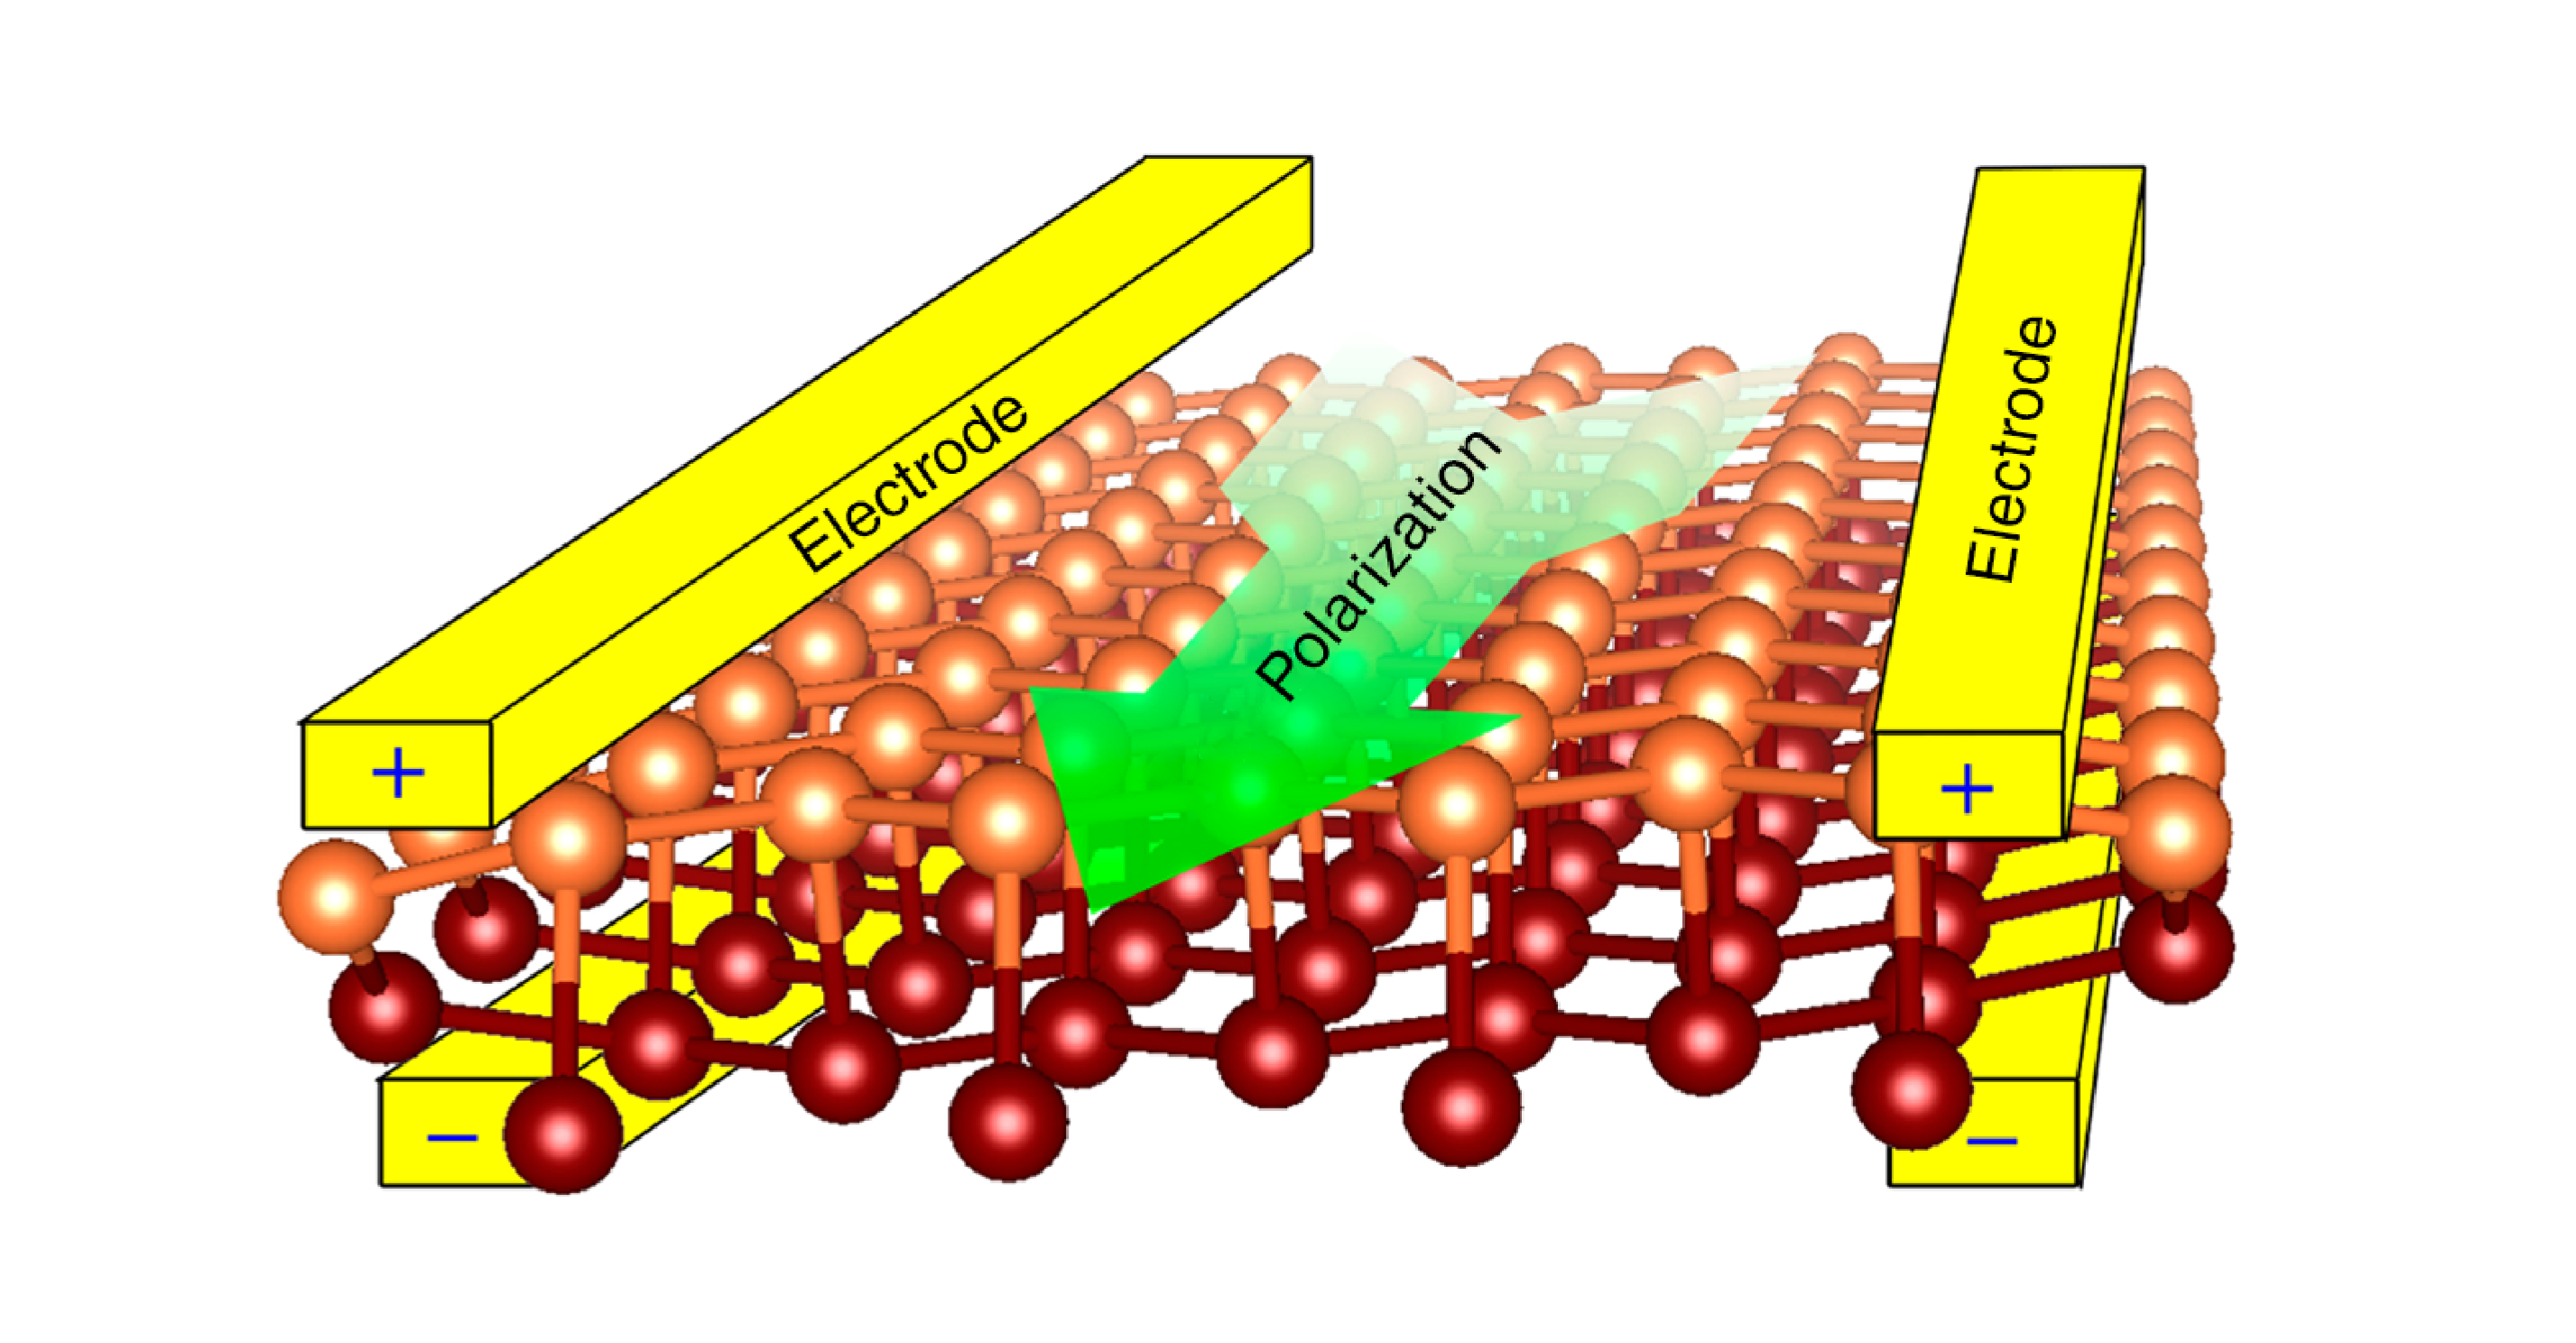
\includegraphics[width=0.8\textwidth]{./pic/013.png}
\caption{二维磷烯结构,垂直平面的外加电场导致平面内部产生电极化}

\label{dog013}
\end{figure}

通常认为,具有铁电性质的材料应该是绝缘体,导体中的自由电荷、载流子会在外加电场的影响下产生定向移动,进而会屏蔽掉外场对物质结构内部的作用,起到了电磁屏蔽的作用,阻碍外部电场对电极化方向的翻转作用。然而,在二维材料等低维材料中,由于几何因素等的限制,情况会有所不同。低维材料的若干个维度缺失会限制载流子对内部结构的电磁屏蔽作用,例如在二维材料中,面内部的粒子结构很难屏蔽垂直平面的电磁场对整个二维平面的影响,从而半导体甚至于导体都有可能出现铁电性。最近发现,两到三层拓扑半导体$WTe_{2}$电极化消失的温度在350K以上,经过第一性原理计算表明,将其置于两层石墨烯之间可进一步增强$WTe_{2}$二维层状结构在室温下的稳定性。

既然简单的只有一到两种元素组成的二维材料存在铁电性,更复杂的由多种元素组成的二维材料同样具有铁电性。过渡金属硫代磷酸酯(transition metal thiophosphate,TMTP)这类复杂的二维材料同样具有铁电性,这类复杂的二维材料的铁电性通常是由金属阳离子的位移与空间晶格扭曲引起的。$ AgBiP_{2}Se_{6}$对可见光有强吸收,可以作为光催化剂应用在水在光下分解等场合。

\subsection{诱导产生铁电性的二维材料}

除了二维材料本身带有的固有铁电性,一些二维材料可以被外围条件诱导产生铁电性。常见的诱导方式有吸附、应力和外场。二维材料具有巨大的表面积,十分容易吸附一些其余的原子分子离子。石墨烯吸附羟基官能团后面内会产生电极化,这与质子位移有关。一系列的二维材料例如硅烷、锗烷、$MoS_{2}$分子层等,吸附一些自组装官能团(OH,SH,CH3,CF3,NH2等)之后,会在面内产生电极化。外加吸附上去的分子很大可能会破坏了平面内的对称性,导致了特殊方向的出现。同样的,外加应力也会导致平面内部的对称性破缺,从而引发电极化,例如PbTe,适当的二维压缩会是其从正常相向铁磁相转化。对于磷烯纳米层,在垂直平面方向上施加电场会导致在面内出现电极化。

\begin{figure}[h]
    \centering
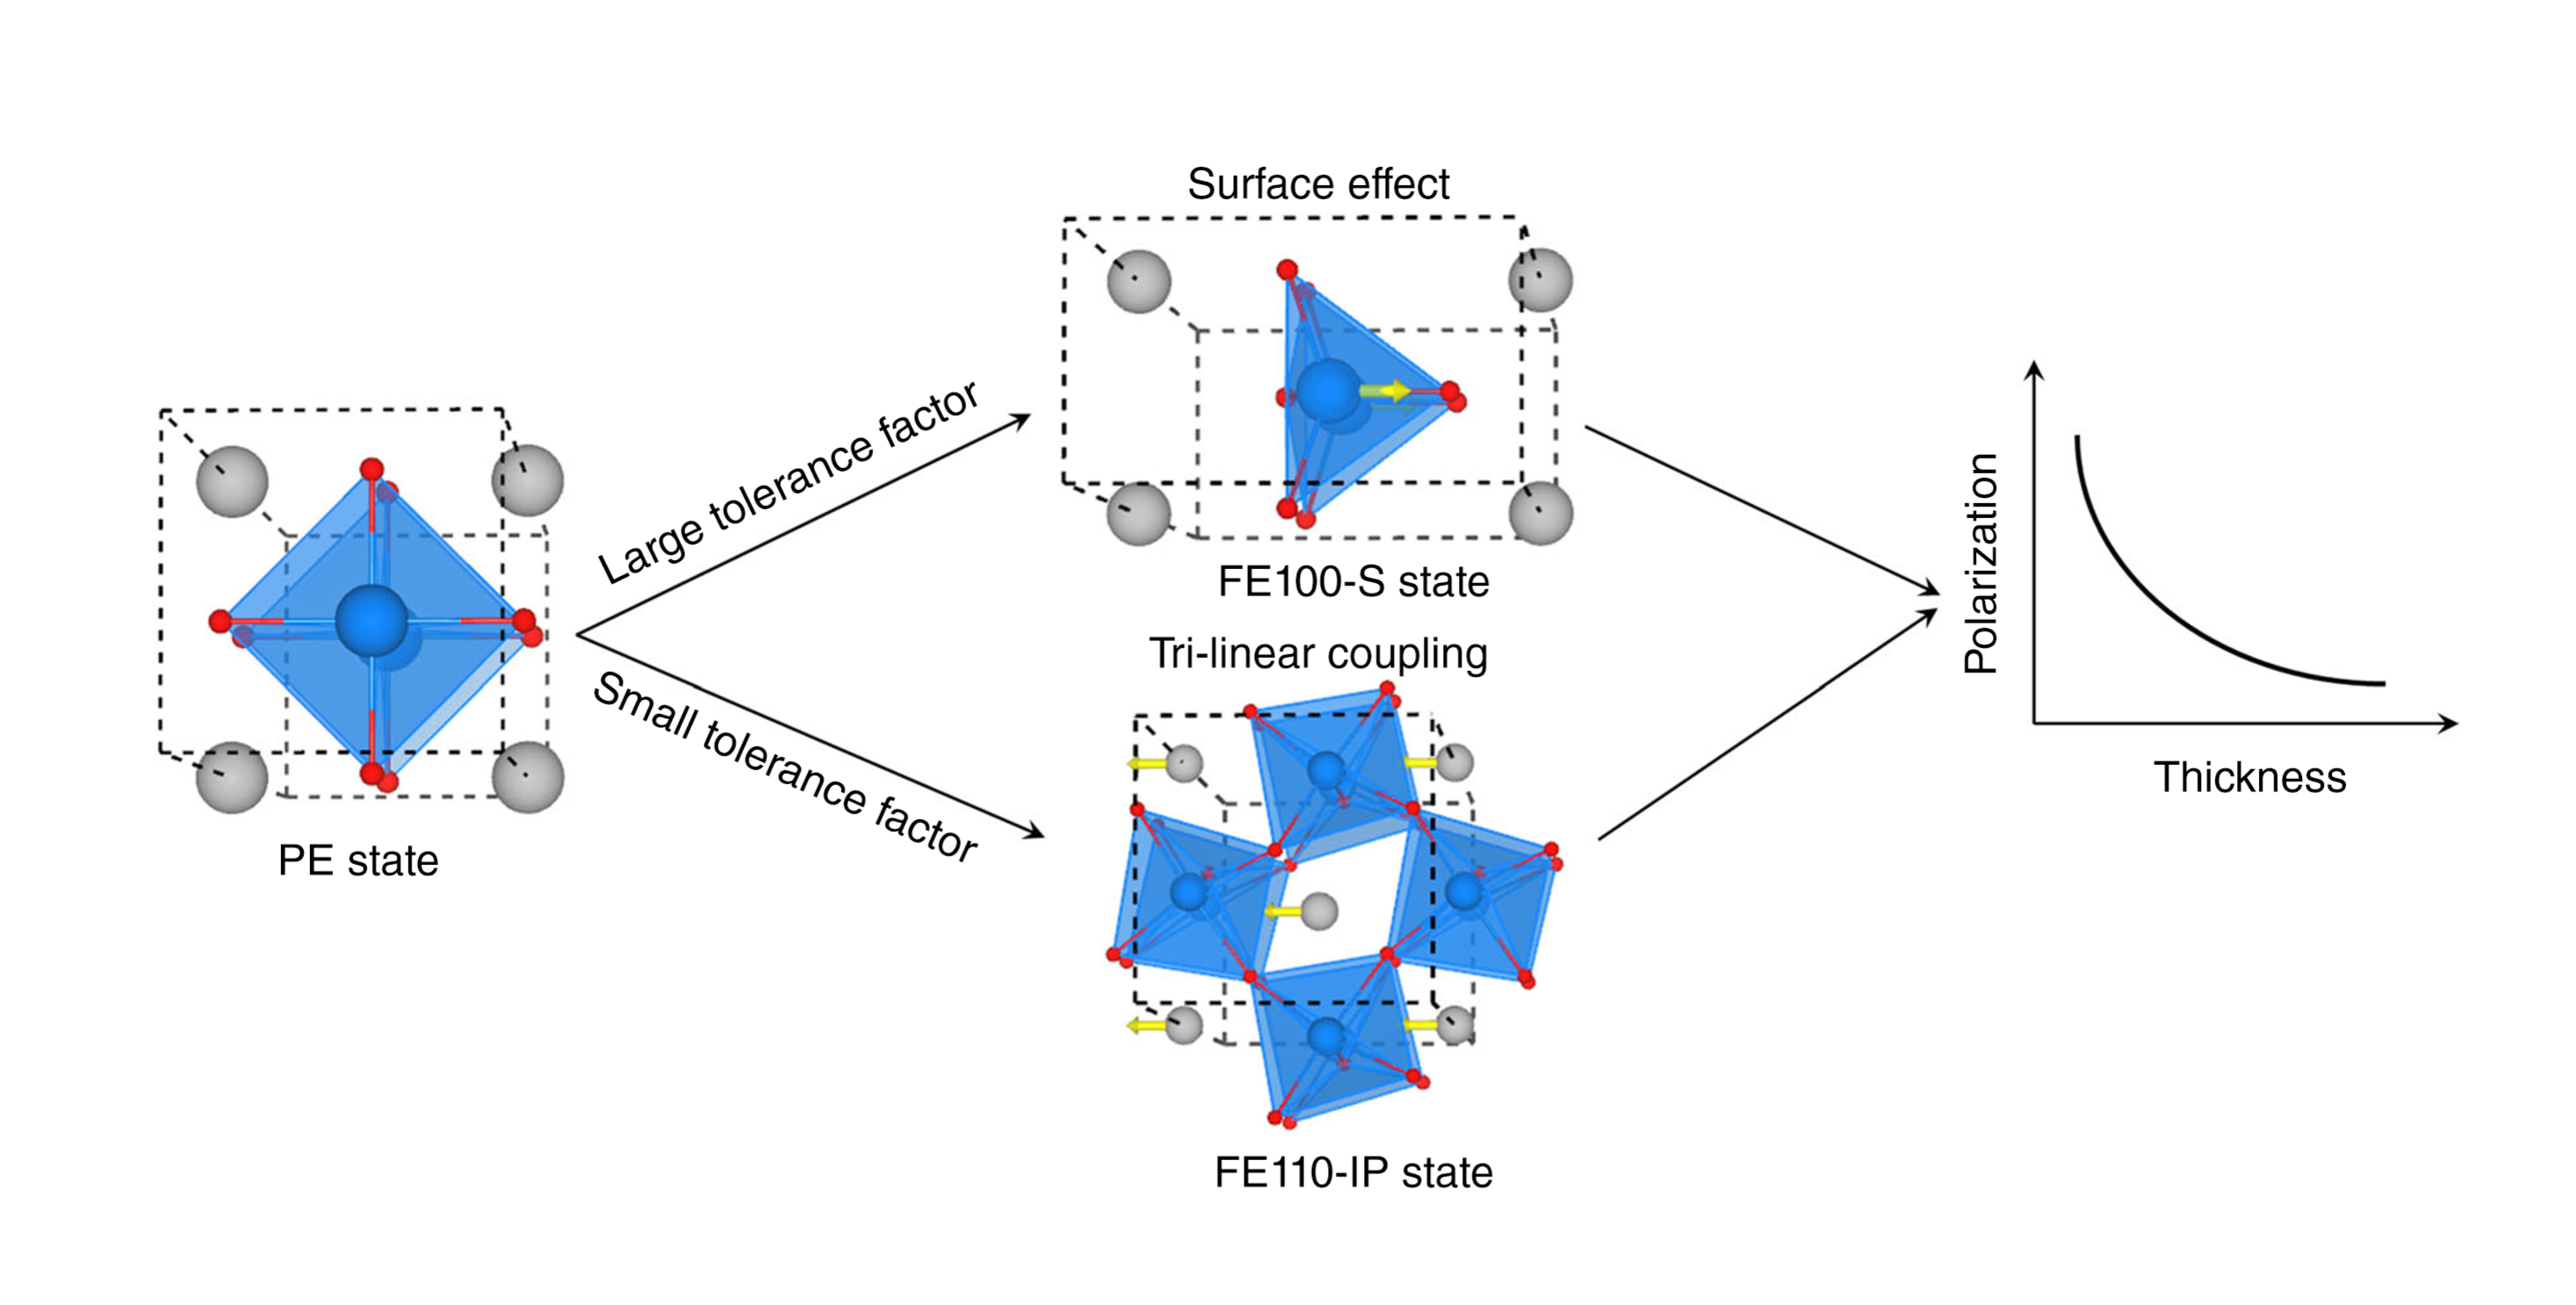
\includegraphics[width=0.8\textwidth]{./pic/014.png}
\caption{二维钙钛矿结构薄膜之中两种不同的氧八面体扭曲结构形成的铁电相,不同的扭曲方式与金属阳离子的半径有关,整个二维体系的铁电性随厚度的减小而增强}

\label{dog014}
\end{figure}

\subsection{基于钙钛矿结构的铁电材料}

在通常的三维材料之中$ABO_{3}$形式的钙钛矿结构通常是铁电压电研究领域的常见材料,在二维条件下,钙钛矿结构的铁电材料有着极大的研究价值。将在三维体系之中表现良好的钙钛矿结构经过降维之后应用在二维材料之中也是一种不错的思路。对于典型的$ABO_{3}$钙钛矿结构,扭曲结构系数$t=(r_{A}+r_{O}/\sqrt{2}(r_{B}+r_{O}))$,是一个衡量钙钛矿结构扭曲形变的一个重要参数,其中r是钙钛矿中各个粒子的经典半径。如果t比一小,氧八面体会发生明显的倾斜以适应扭曲的晶格结构和失调的原子半径比例所造成的键错配。高对称性晶格结构发生扭曲导致对称性降低是产生铁电性的关键。

\begin{figure}[h]
    \centering
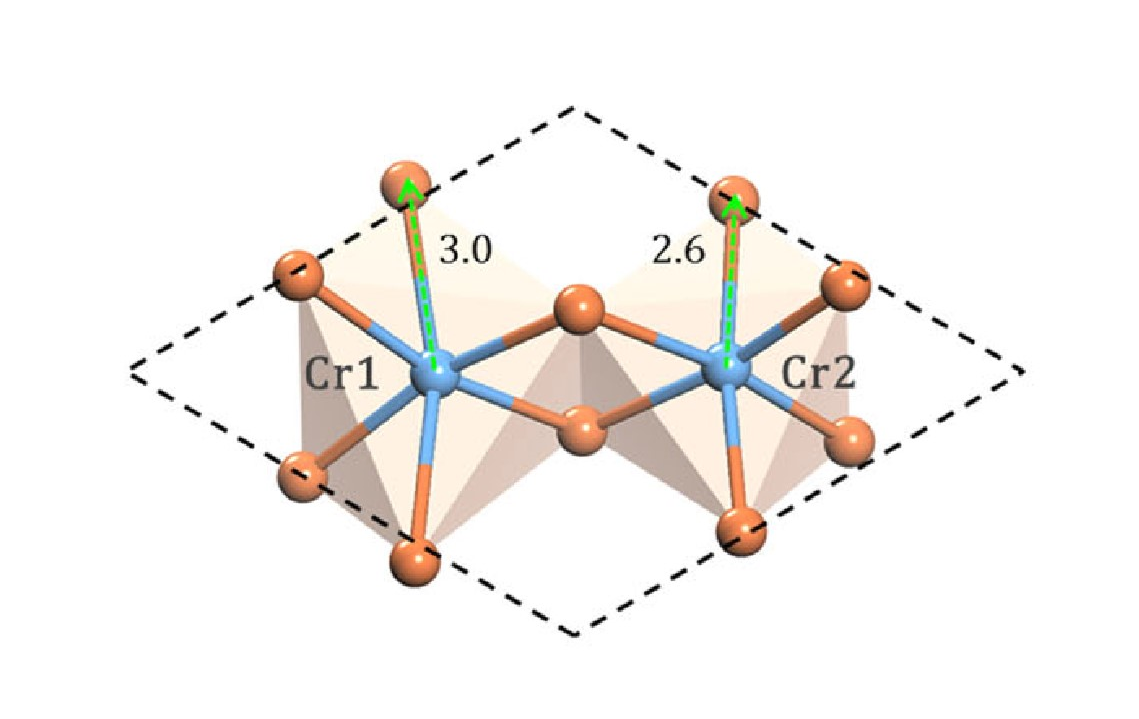
\includegraphics[width=0.8\textwidth]{./pic/010-3.png}
\caption{掺杂电子后的$CrBr_{3}^{0.5-}$结构,电子掺杂使两个$Cr^{3+}$出现差异,地位不在平等,与周围溴离子的键参数发生变化}

\label{dog010-3}
\end{figure}

\section{二维多铁材料的研究背景}

与三维多铁材料一样,二维多铁材料也可以分为两种类型。第一类多铁体的铁磁铁电性质来源不同,第二类二维多铁材料的铁磁铁电性质有着相同的来源。\cite{wang2009multiferroicity:,dong2015multiferroic} 一般来说,第一种的电磁耦合比较弱。而第二类多铁体通常是由于磁有序导致空间的中心对称性破缺,从而出现电极化,这类电磁同源二维多铁材料电磁耦合强,但是电极化很小且温度很低。由于铁电与铁磁效应的内在排斥,很难发现二维多铁材料。

对于已经存在铁电性的二维材料,将其改造为多铁材料最方便有效常用的方法是掺杂磁性元素或过渡金属。对于石墨烯或者其他的一些类似的二维材料,掺杂一些非磁性的元素周期表靠前的元素(H、F),导致费米面附近电子浓度增加,同样也可以产生铁磁性。

目前已将预测或发现了多种的单独存在铁电性与铁磁性的的二维材料。其中二维铁电材料主要有$MoS_{2}$ \cite{yuan2019room-temperature} 、石墨烯 \cite{kan2013high-temperature} 、$SnSe$ \cite{fei2016ferroelectricity} 等二维材料。在二维过渡金属卤化物中也观测到了铁磁性。\cite{huang2017layer-dependent} 通常大部分过渡金属卤化物是磁性半导体或者绝缘体,这给在过渡金属卤化物之中寻找同时存在的铁电性与铁磁性提供了可能。

通过第一性原理计算,卤素修饰磷烯双层可能是带有垂直平面的电极化与可移动磁矩的多铁材料。卤素原子在两层见形成的共价键破坏了两层的对称性,卤素原子在上下两层的结合的改变导致了电极化方向的翻转。磁矩直接来源于卤素原子,每个卤素原子可以提供1$\mu_{B}$的磁矩
,磁矩的方向可以被外加电场的方向改变,这一性质使得这种材料有希望被应用在磁读电写存储器上。

带有乙醚基官能团的锗烯也是一种同时具有铁磁性与铁电性的二维材料。其铁电性来源于极化配体乙醚基在面内的旋转,平面上没有被官能团化的锗原子$p_{z}$轨道上的一个未配对电子提供了1$\mu_{B}$的磁矩。

从另一方面看,对二维铁磁材料进行适当的调整或设计也可以产生多铁性。对于很多过渡金属组成的低维结构,加入一些可以导致对称性破缺的官能团有可能会出现电极化。从实现电极化的翻转难易程度上考虑,通常会添加一些自身带有极化或者强电负性官能团,例如$-F,-Cl,-CN,-NO_{2},=O,-OH \text{或}-COOH $。这类情况通常出现在有机二维网状结构之中,二维$C_{6}N_{8}H$网状结构,质子的输运会导致电极化在两种不同的方向间切换,质子打破了碳氮化物的对称性,使其自旋密度分布各向异性,铁电性与铁磁性之间也发生了耦合。

一般认为铁电性不会出现在具有强铁磁性的金属中,即使金属中存在有微观的电极化,金属中的自由电子会屏蔽掉外电场对自发极化电矩的作用,从而在宏观层面无法表现出铁电性,但在二维材料之中,垂直平面的电极化却很难被面内运动的自由电子屏蔽从而受到垂直平面电场的影响。第一性原理计算表明,具有二维铁磁性的CrN存在垂直平面的电极化,自旋声子耦合使得其内部的铁磁性与铁电性耦合起来。$CrB_{2}$是一种可以用电场调控铁磁性的二维材料,在垂直平面方向施加一个大电场可以使其从反铁磁状态转化为铁磁铁电状态,而一个相对较小的状态可以将其转化回到原来的反铁磁状态。

现在发现的二维多铁材料大多都是第一类多铁材料,第一类多铁材料的电磁耦合强度比较小,为了获取较强的的电磁耦合,需要设计制作第二类多铁材料,即铁电铁磁同源的二维材料。受限于客观条件,这类多铁材料一般很难发现。双过渡金属碳化物$Hf_{2}VC_{2}F_{2}$,是一种第二类二维多铁材料,其120°Y型自旋序打破了空间对称性并产生了一个垂直自旋平面的电极化,但是这个电极化强度过小,只有$ 2.9 × 10^{−7}μC/m$,远小于其他的多铁二维材料。

\begin{table}[!htbp]
    \caption{常见的二维多铁材料}
    \label{tab:dog}
    \resizebox{\textwidth}{!}{
    \begin{tabular}{llllllc}
        \toprule
        
        材料 & 极化强度(pC/m) & 电极化方向 & 磁矩($\mu_{B}$)& FE switch barrier(meV/f.u.) & 转变温度(K) &参考资料 \\
        \midrule
        Phosphorene-halogen&~11&Out-of-plane&1.0&74–590&~572&\cite{yang2017chemically}\\
        Ge-CH2OCH3&~80&In-plane&1.0&~100&—&\cite{kou2018multiferroic}\\
        C6N8H3&6.3–45&In-plane&1.0&70–480&250–700&\cite{tu2017two}\\
        Bilayer Cr2NO2,VS2, MoN2&—&Out-of-plane&0.008–0.09&—&—&\cite{li2017binary}\\
        CrN&6.2&Out-of-plane&3&12&—&\cite{luo2017two}\\
        % CrB&20.9&Out-of-plane&1.5&363&&\\
        CuMP2X6(M = Cr, V; X = S, Se)&0.65–0.79&Out-of-plane&2.0-3.0&27–100&—&\cite{qi2018two}\\
        (CrBr3)2Li&92&In-plane&3.0, 4.0&15&—&\cite{huang2018prediction}\\
        SrMnO3&55μC/cm2&In-plane&—&—&Above 420&\cite{guo2018strain}\\
        Hf2VC2F2&2.9× 10−7&Out-of-plane&2.04&—&313&\cite{zhang2018type}\\


        \bottomrule
    \end{tabular}}
\end{table}

\section{典型的多铁二维材料}

\subsection{溴化铬多铁性产生原理}

二维溴化铬系统中的铁电性可以由电荷排序与轨道排序引发。通过计算表明,在溴化铬二维结构之中掺杂一个电子,通过晶体场理论中的杨-泰勒效应使对称性破缺,两个相邻的$Cr-Br_{6}$单元会产生电荷排序与轨道排序。从而导致二维溴化铬产生多铁性。



三维系统中的电荷排序或者轨道排序都可以独立的产生铁电性,但在二维系统之中,单独的电荷排序并不一定引起对称性的破缺,从而产生电极化。\cite{zhou2014carrier}没有掺杂的二维溴化铬是没有极化现象的铁磁体,当掺杂空穴时对称性没有被破坏,不会产生极化现象。但掺杂电子时,JT效应会使相邻的Cr原子产生不同的能级分裂,导致电子的分布不同,从而产生铁电性。从能带论上面来看,掺杂电子会使费密能级提高,从而使Cr-e态被部分占据,进而使JT扭曲效应出现,破坏对称性。\cite{BENGEL199595} 

\begin{figure}[h]
    \centering
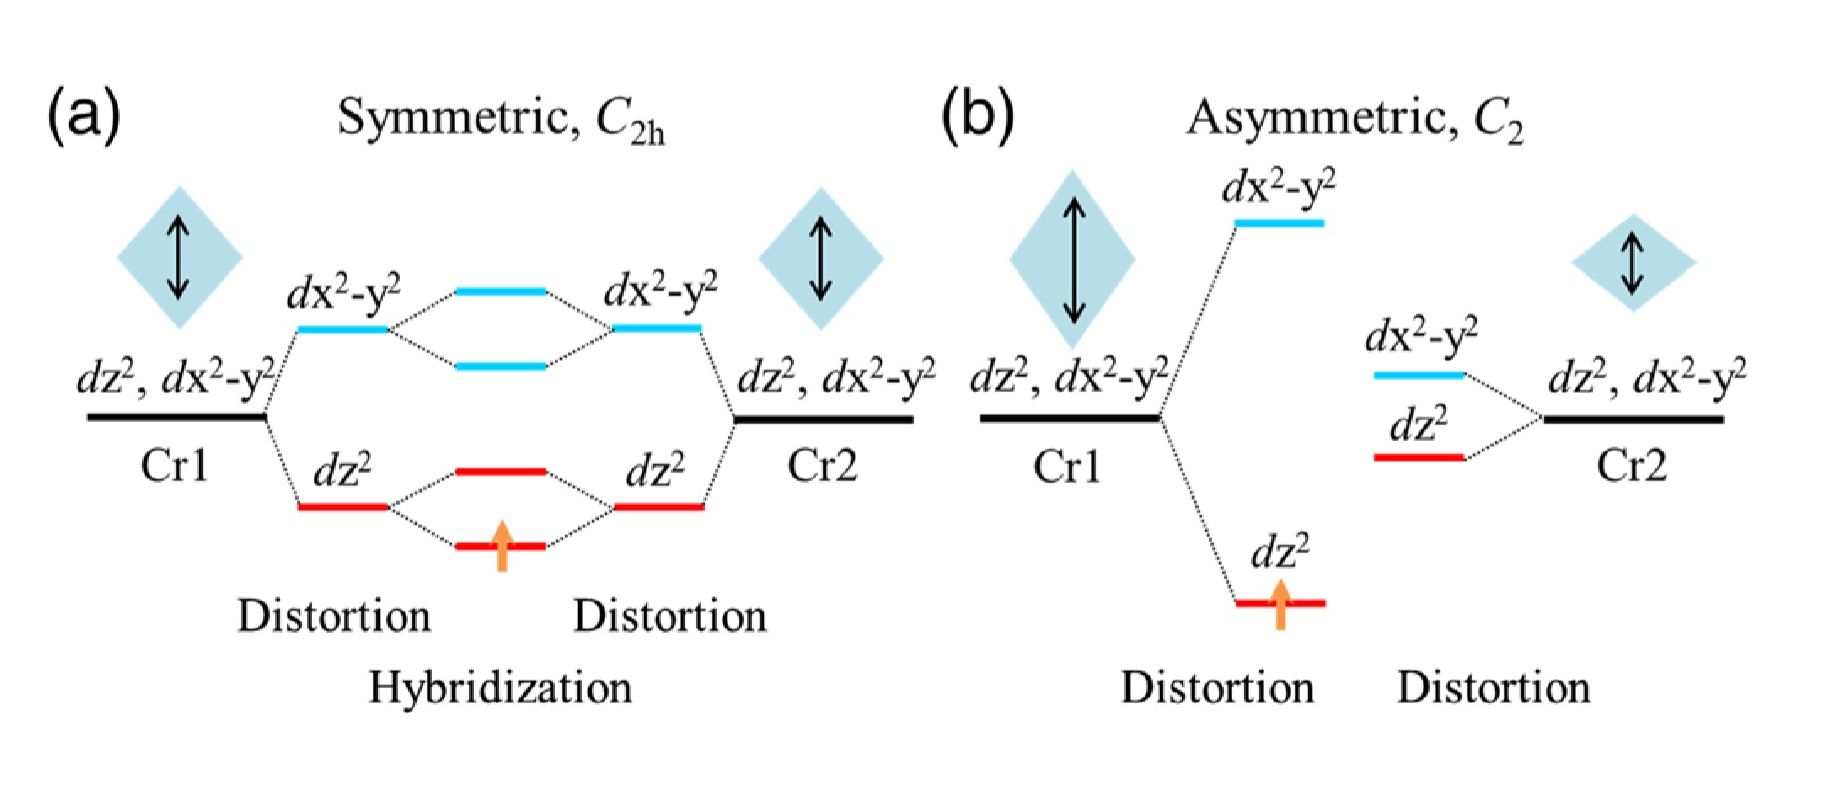
\includegraphics[width=0.8\textwidth]{./pic/011-2.png}
\caption{在不同对称性破缺下,JT效应产生的简并分裂情况不同}

\label{dog011-2}
\end{figure}

在二维溴化铬之中,一个平行四边形基元内部有两个铬离子。在未经掺杂的溴化铬二维层状结构中,只存在铁磁性,没有极化现象。在掺杂空穴的$CrBr_{3}^{x+}$之中,垂直二维平面的对称性没有被破坏。而在电子掺杂的$CrBr_{3}^{x-}$之中,JT效应会使晶格空间结构发生畸变,然后在$C_{2}$对称轴(面内对称轴,详见图)方向,出现电极化。从能带论上面看来,空穴掺杂会使系统的费米面降低,到达Br-p轨道附近,这样就不能引发JT效应使对称性破缺。掺杂电子时,费米面会升高,到达Cr-e轨道附近,所引起的JT扭曲效应会使对称性破缺,从而产生出一个允许电极化存在的特殊方向。对于$CrBr_{3}^{0.5-}$,在平行四边形基元内部,两个Cr并不是完全等价的,Br-Cr键长在垂直于平面的方向有着大约0.4A的差距,这在普通的过度金属卤化物是十分异常的。通过计算表明,$CrBr_{3}^{0.5-}$这种反对称的畸变比对称性的畸变和没有产生畸变情况下能量都要低。

$CrBr_{3}^{0.5-}$的电极化来源于JT效应导致的对称性破缺,其铁磁性则来源于作为过渡金属元素的铬离子,铁电性与铁磁性的耦合最终还是要依靠自旋轨道耦合来解释。铁电性的来源是JT效应,归根结底还是原子轨道叠加杂化组合引起的电子密度分布的变化,铁磁性的来源与其他过渡金属元素组成的物质类似,归根结底是电子自旋,这样看来自旋轨道耦合是连接铁磁性与铁电性的关键。

对于$CrBr_{3}^{0.5-}$,JT效应造成能级分裂有两种,一种是对称的,另一种是反对称的,在对称的$C_{2h}-CrBr_{3}^{0.5-}$之中,两个$Cr-Br_{6}$单元发生同样的分裂:一个更高能量的$dx^{2}-y^{2}$轨道和一个更低能量的$dz^{2}$状态。掺杂进来的多的那个电子占据在两个$Cr-dz^{2}$轨道的超杂化态。两个Cr原子完全等价。在反对称的$C_{2}-CrBr_{3}^{0.5-}$,两个$Cr-Br_{6}$扭曲的程度不同,所造成的能级分裂也不同,这就导致了两个Cr的低能级轨道很难进行超杂化,只能占据Cr1的低能量$dz^{2}$。再加上3d轨道的定域性比较强,电子近似可以看作只停留在一个Cr附近。通过对这两种掺杂电子的分裂方式进行计算,反对称方式能量低大约0.8电子伏,这就导致在$CrBr_{3}^{0.5-}$系统中更偏向出现反对称JT效应。

在真实的二维材料之中掺杂电子有很多方法,可以采用合适的基底、掺杂金属或离子。目前已经可以在FeSe薄片中掺杂高比例锂离子进行电子掺杂。\cite{lei2017tuning} 选择$(CrBr_{3})_{2}Li$或许是可行的。 同样对于其他的卤族元素,如氯、碘等元素,与$CrBr_{3}$有着相似的原子电子结构,也具有多铁性。这样的理论在其他的过渡金属卤化物上也适用。

\section{基于四族元素的一硫族化合物的多铁二维材料}

第四主族的一些元素的与S、Se等形成的二维层状化合物具有面内的在室温下可以稳定存在的多铁性,与其他多铁材料不同的是,这类材料的铁性质不是常见的铁磁性与铁电性性,而是铁电性与铁弹性。\cite{wang2017two}\cite{ISI:000088490500004}这类材料不仅有多铁性,而且对可见光谱有着各向异性的强吸收,这意味着有可能透过光场对材料的多铁性质进行调控。这种铁电性、铁弹性与光学性质耦合的多铁二维材料在制备二维可调控多铁器件与铁电存储器方面有着巨大的潜力。
\begin{figure}[h]
    \centering
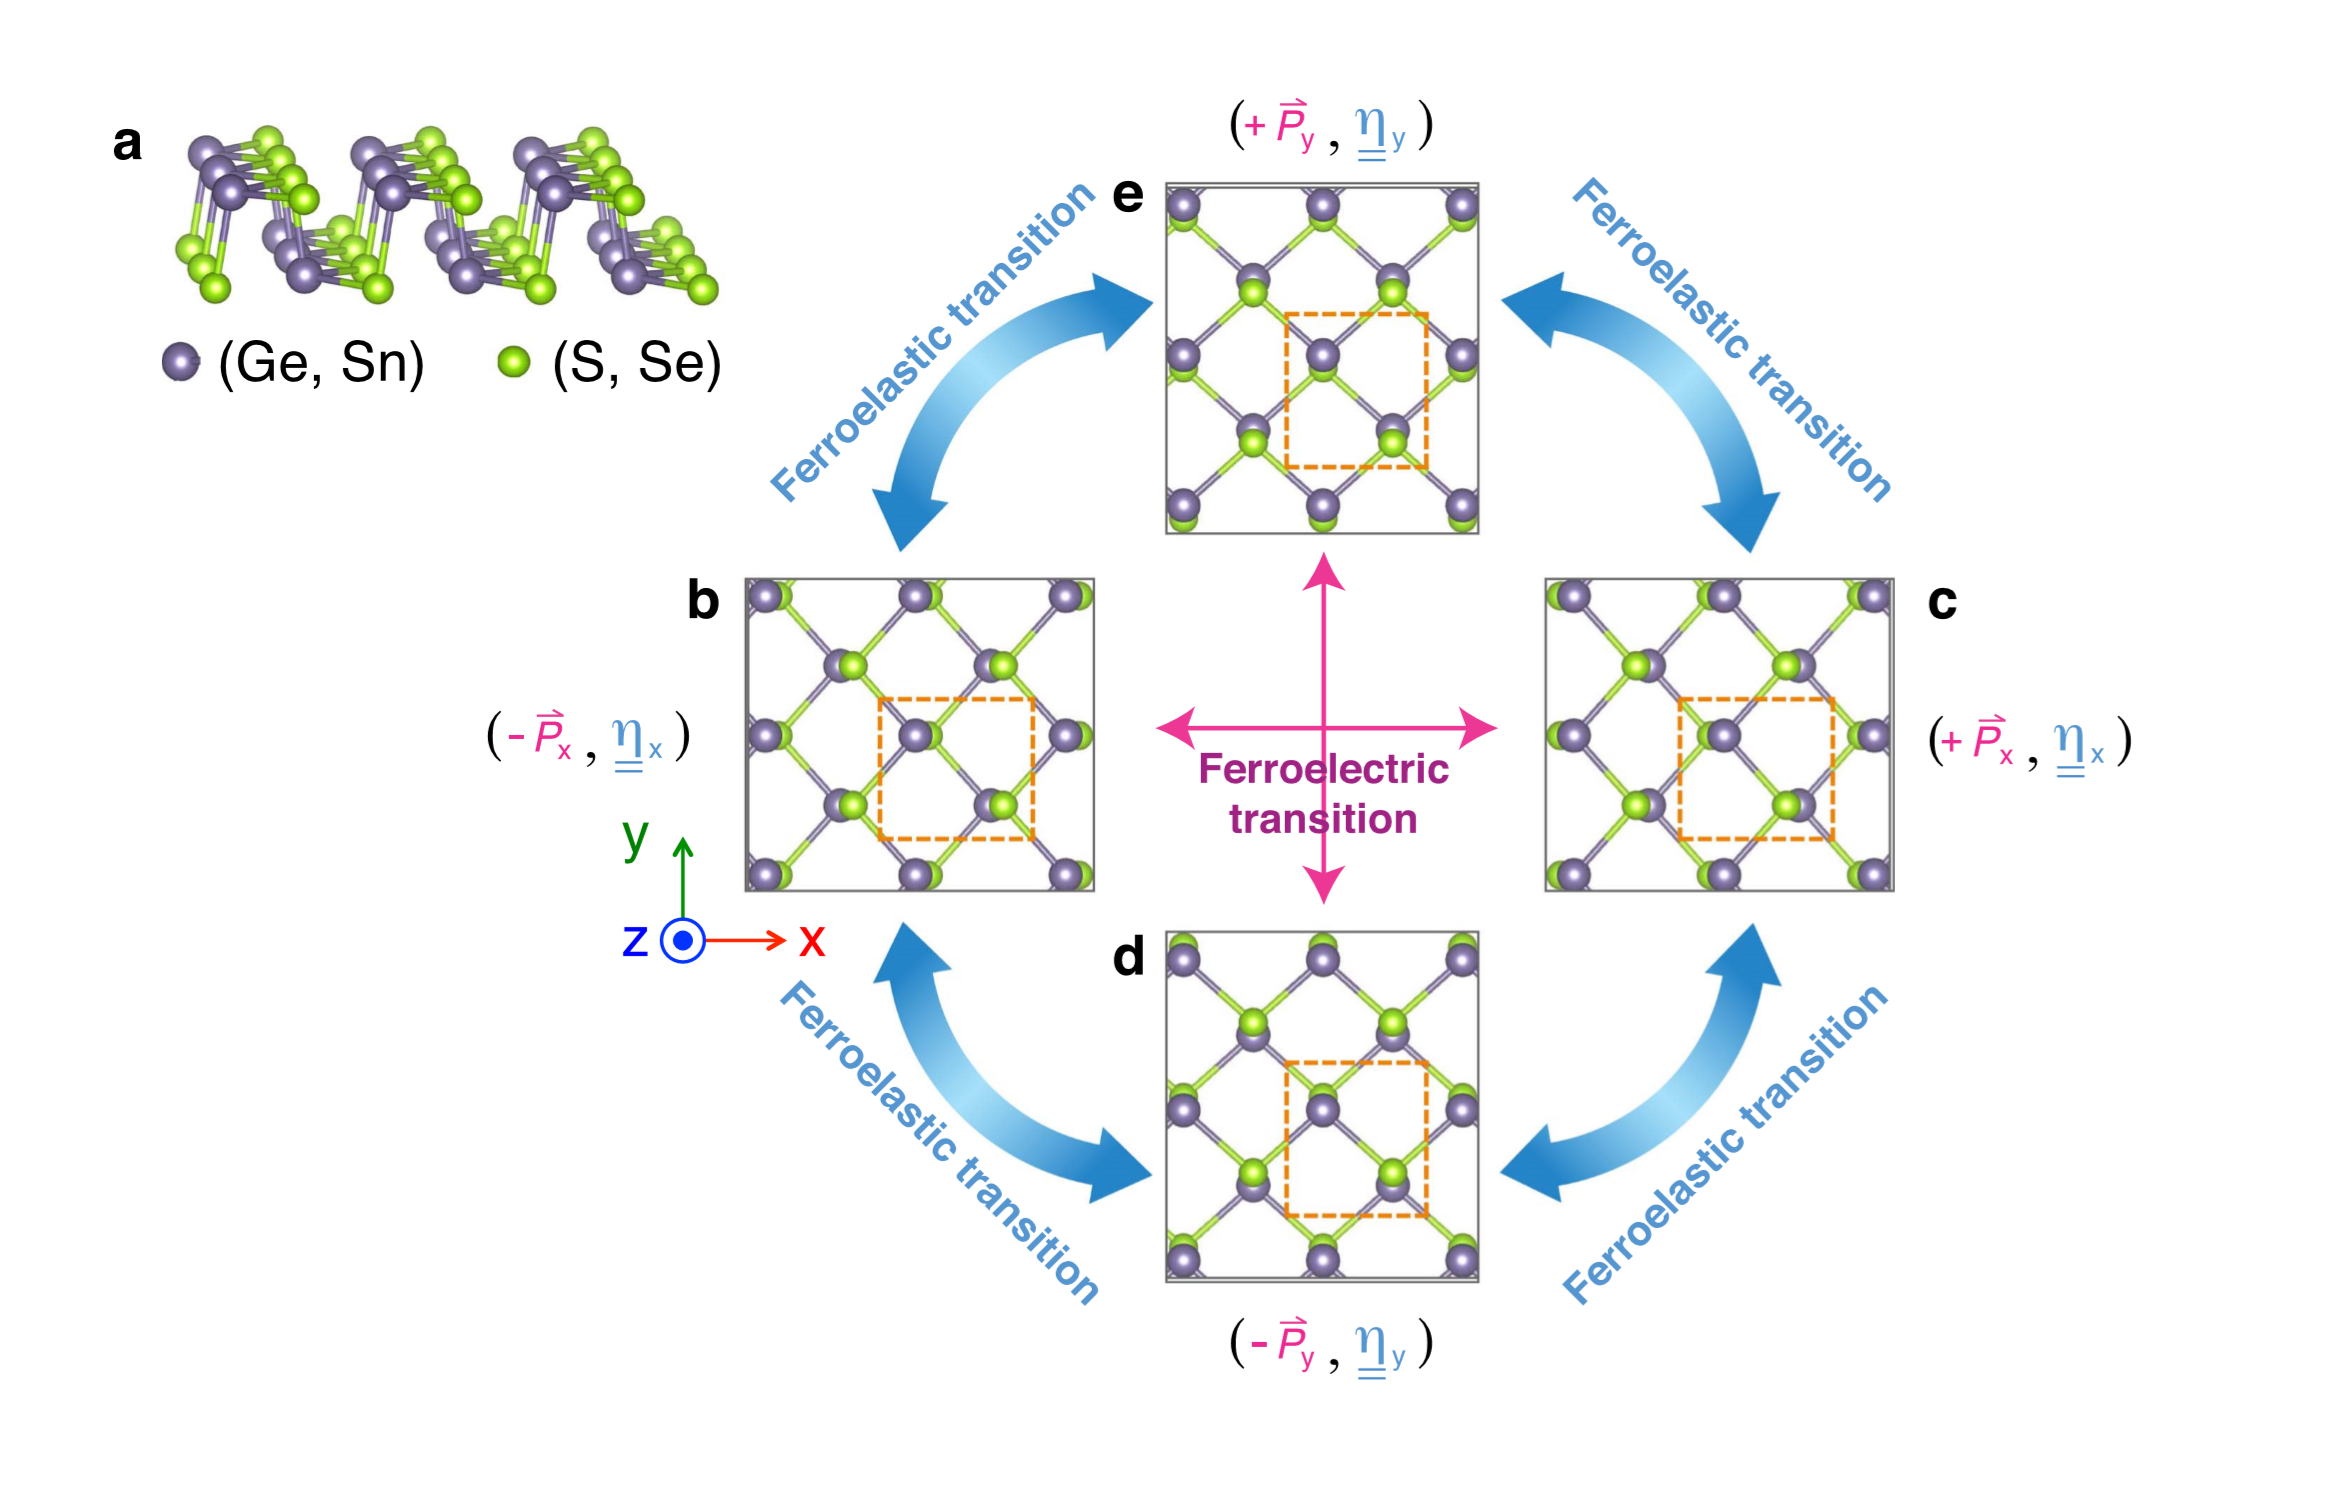
\includegraphics[width=0.8\textwidth]{./pic/018.png}
\caption{MX二维分子层状结构与面内的铁电性与铁弹性\ 分子层内部有四种电极化方向,沿着X轴有两种电极化状态$P_{x}\text{和}-P_{x}$,沿着Y轴也有两个电极化状态$P_{y}\text{和}-P_{y}$ \ 有两种铁弹性状态$\eta_{x}\text{和}\eta_{y}$这四种状态可以通过铁电性与铁弹性进行相互转化}

\label{dog018}
\end{figure}

作为一大类二维多铁材料\cite{ISI:000230853300010},四族元素的一硫族化合物(主要包括GeS, GeSe, SnS ,SnSe等)有着相似的结构,同样拥有强耦合的多铁性。\cite{ISI:000318143300005}\cite{ISI:000309505400023}可以认为。多铁性在这些材料中是普遍存在的。这类二维材料的铁弹性与二维晶格两个垂直方向的形变有关,晶格扭曲导致内部正负电荷中心发生位移,进而导致材料内部电极化发生变化,铁弹性是与铁电性直接耦合的,这支持了采取外场对另一种铁性质进行调控的可能。

\subsection{铁弹性与自发应变}

四族元素的一硫族化合物通常可以表示为MX,其中M可以是Ge、Sn,X是S 、Se。以GeSe为例,GeSe的单层结构如图所示,其铁弹性起源于其晶格结构沿x和y方向发生自发弛豫,晶格移动形变的方向不同。\cite{ISI:000363915300044}通过计算表明,稳定的层状机构并不是在XY方向对称的,在一个方向压缩与另一个方向拉伸。压缩与拉伸的方向不同可以分成两个相,二既不拉伸又不压缩的中间状态能量比较高,这就形成了一个势垒。如果有外加影响如外场或者外加应力,会是一个相越过中间的势垒转化到另一个相。微观机构的晶格参数的改变在宏观层面表现出来就是几何外形与尺寸的改变。从对称性来看。在平面内部XY方向的对称性被破坏,其中一个方向变得特殊起来,各种铁性质的出现与对称性的破缺有着密切的关系。

\begin{figure}[h]
    \centering
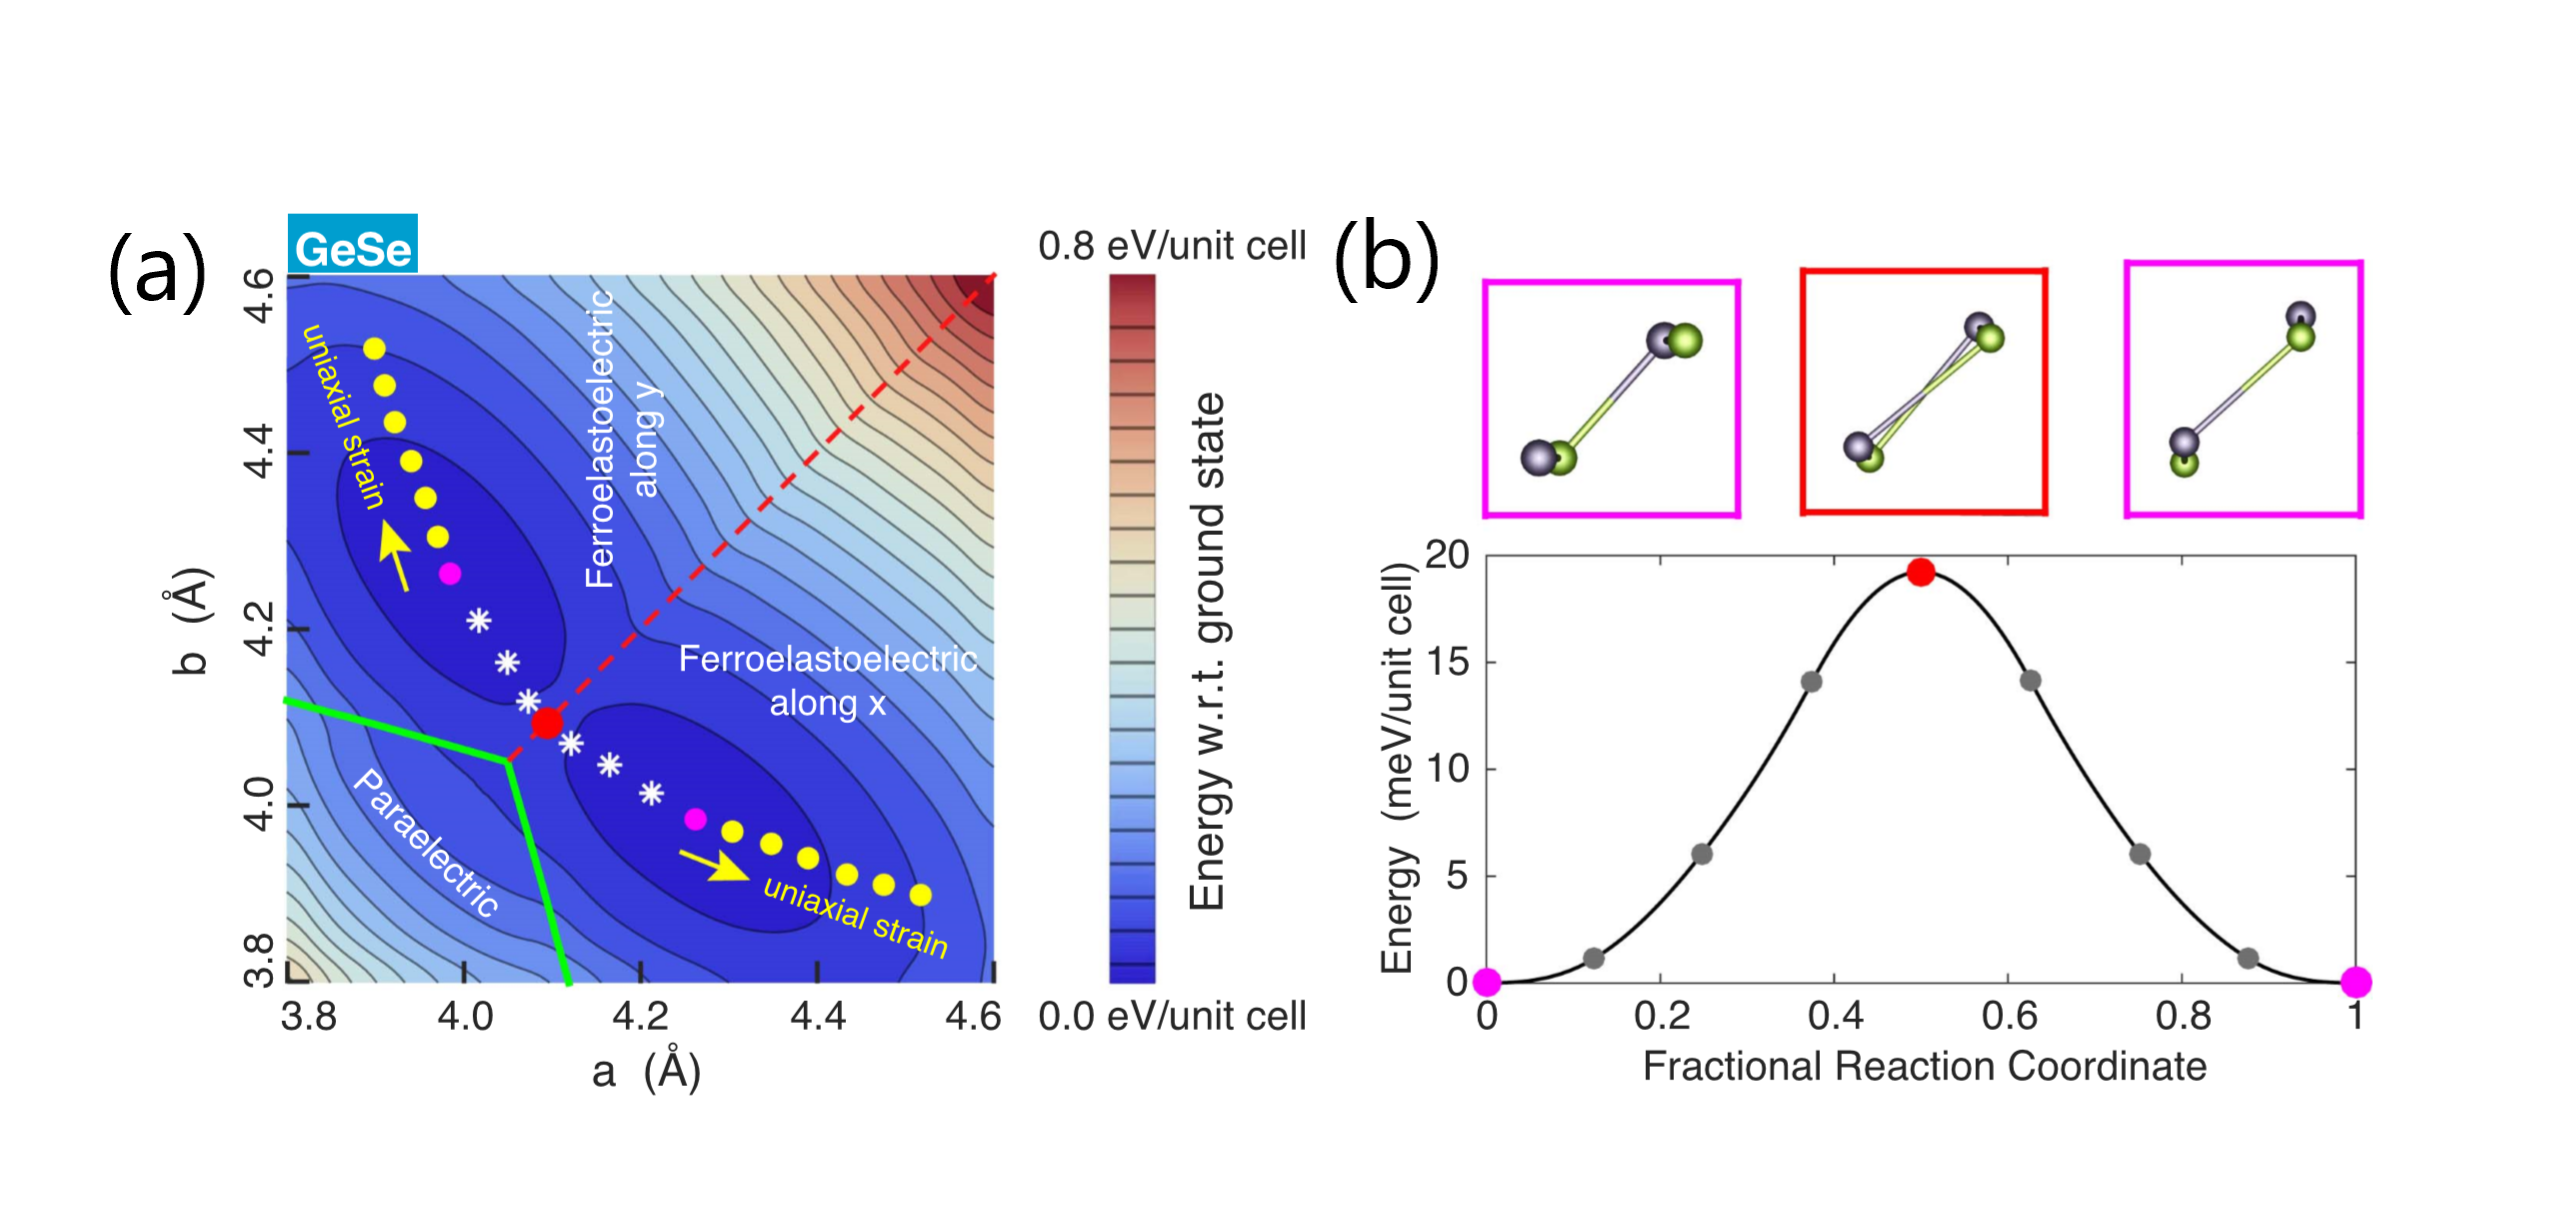
\includegraphics[width=0.8\textwidth]{./pic/017.png}
\caption{(a)不同晶格常数下GeSn的总能量\ 可以从图上看到,有着一个高对称性顺弹性相,位于势能的曲面的鞍点,并不是一个能量最低的稳定态,两个稳定态是两个不同的铁弹性太,具有自发的应变。(b)两个铁弹性态之间转换的最低能量路径,从图中可以看出,两种状态之间的转换并没有经过高对称性的顺弹性状态,而是通过层状结构上下原子位置的相对转动从一种状态转化到另一种状态。}

\label{dog017}
\end{figure}

进一步的计算表明,对称性较高的顺弹性的态是亚稳态其晶格常数可以用矩阵$\bm{H}_{ref}=\begin{bmatrix}
    &4.1&0\\
    &0&4.1
\end{bmatrix}$表示。选取高对称顺弹性状态$\bm{H}_{ref}$作为参考,两种低对称性的状态分别为$\bm{H}_{x}=\begin{bmatrix}
    &4.26&0\\
    &0&3.98
\end{bmatrix}$和$\bm{H}_{y}=\begin{bmatrix}
    &3.98&0\\
    &0&4.26
\end{bmatrix}$
相对于基准状态,两种状态的转换应变矩阵:
\begin{equation}
    \begin{split}
        &\eta_{x}=\frac{1}{2}([H_{ref}^{-1}]^{T}H_{x}^{T}H_{x}H_{ref}^{-1}-\bm{I})\\
        &\eta_{y}=\frac{1}{2}([H_{ref}^{-1}]^{T}H_{y}^{T}H_{y}H_{ref}^{-1}-\bm{I})\\
        &\eta_{x}=\begin{bmatrix}
            0.041&0\\
            0&-0.027
        \end{bmatrix}\\
        &\eta_{y}=\begin{bmatrix}
            -0.027&0\\
            0&0.041
        \end{bmatrix}
    \end{split}
    \label{eq:txxb}
\end{equation}
对于$\eta_{x}$,这表示在X方向发生了4.1\%的拉伸,在Y方向发生了2.7\%的压缩。同样地对于$\eta_{y}$,这表示在Y方向发生了4.1\%的拉伸,在X方向发生了2.7\%的压缩。虽然在两种铁弹性相之间有着一个顺弹性势垒,但在这两种铁弹性状态转变时,却不会经历中间的顺弹性状态。而是通过两种原子的相对旋转实现的。

\subsection{铁电性与自发极化}
虽然铁电与铁弹性有着密切的关系,都存在着空间范畴上的对称性破缺,但这两点又有着区别与不同。铁电性是正负电荷中心自发偏离,形成空间中的电偶极子与自发极化。在自发极化方向翻转时不一定会产生宏观层面的晶格形变,反之在晶格结构发生变化时,自发极化、正负电荷中心也不一定随之发生变化。对于像GeSe这样铁弹性与铁电性强耦合的材料,其内部有着及其密切的关系。基于量子绝热定理,可以通过几何相位导出自发极化强度的表达式:
\begin{equation}
    \begin{split}
        \bm{P}_{s}&=\bm{P}^{f}-\bm{P}^{i}\\
        &=\frac{1}{\Omega}\sum_{j}(q^{f}\bm{r}^{f}-q^{i}\bm{r}^{i})-\frac{2ie}{(2\pi)^{3}}\sum_{n}^{occ} [ \int_{BZ}d^{3} \bm{k} e^{-i\bm{k \cdot R}} \\
        & \times \langle u^{f}_{n \bm{k}} | \frac{\partial u_{n \bm{k}}^{f}}{\partial \bm{k}} \rangle - \langle u^{i}_{n \bm{k}} | \frac{\partial u^{i}_{n \bm{k}}}{\partial \bm{k}} \rangle ]
    \end{split}
    \label{eq:}
\end{equation}
其中i,j分别表示在量子绝热理论中的出=初状态与末状态。
通过第一性原理计算,GeSn具有强烈的铁弹性与铁电性的耦合。例如当单轴应变增大6\%时自发极化从357pC/m增加到430pC/m。

\subsection{各向异性的光学性质}

通过应用DFT等手段对GeSn等材料的能带结构的计算,MX单分子膜是具有2.6ev-1.1ev间接带隙的二维半导体材料。二维平面内的电极化会导致在二维分子平面内部不同方向的介电常数不同,会导致对不同偏振方向的光产生不同的响应。利用这一点可以采用可见光照射的方式读取二维材料的铁电、铁弹性状态。
\begin{figure}[h]
    \centering
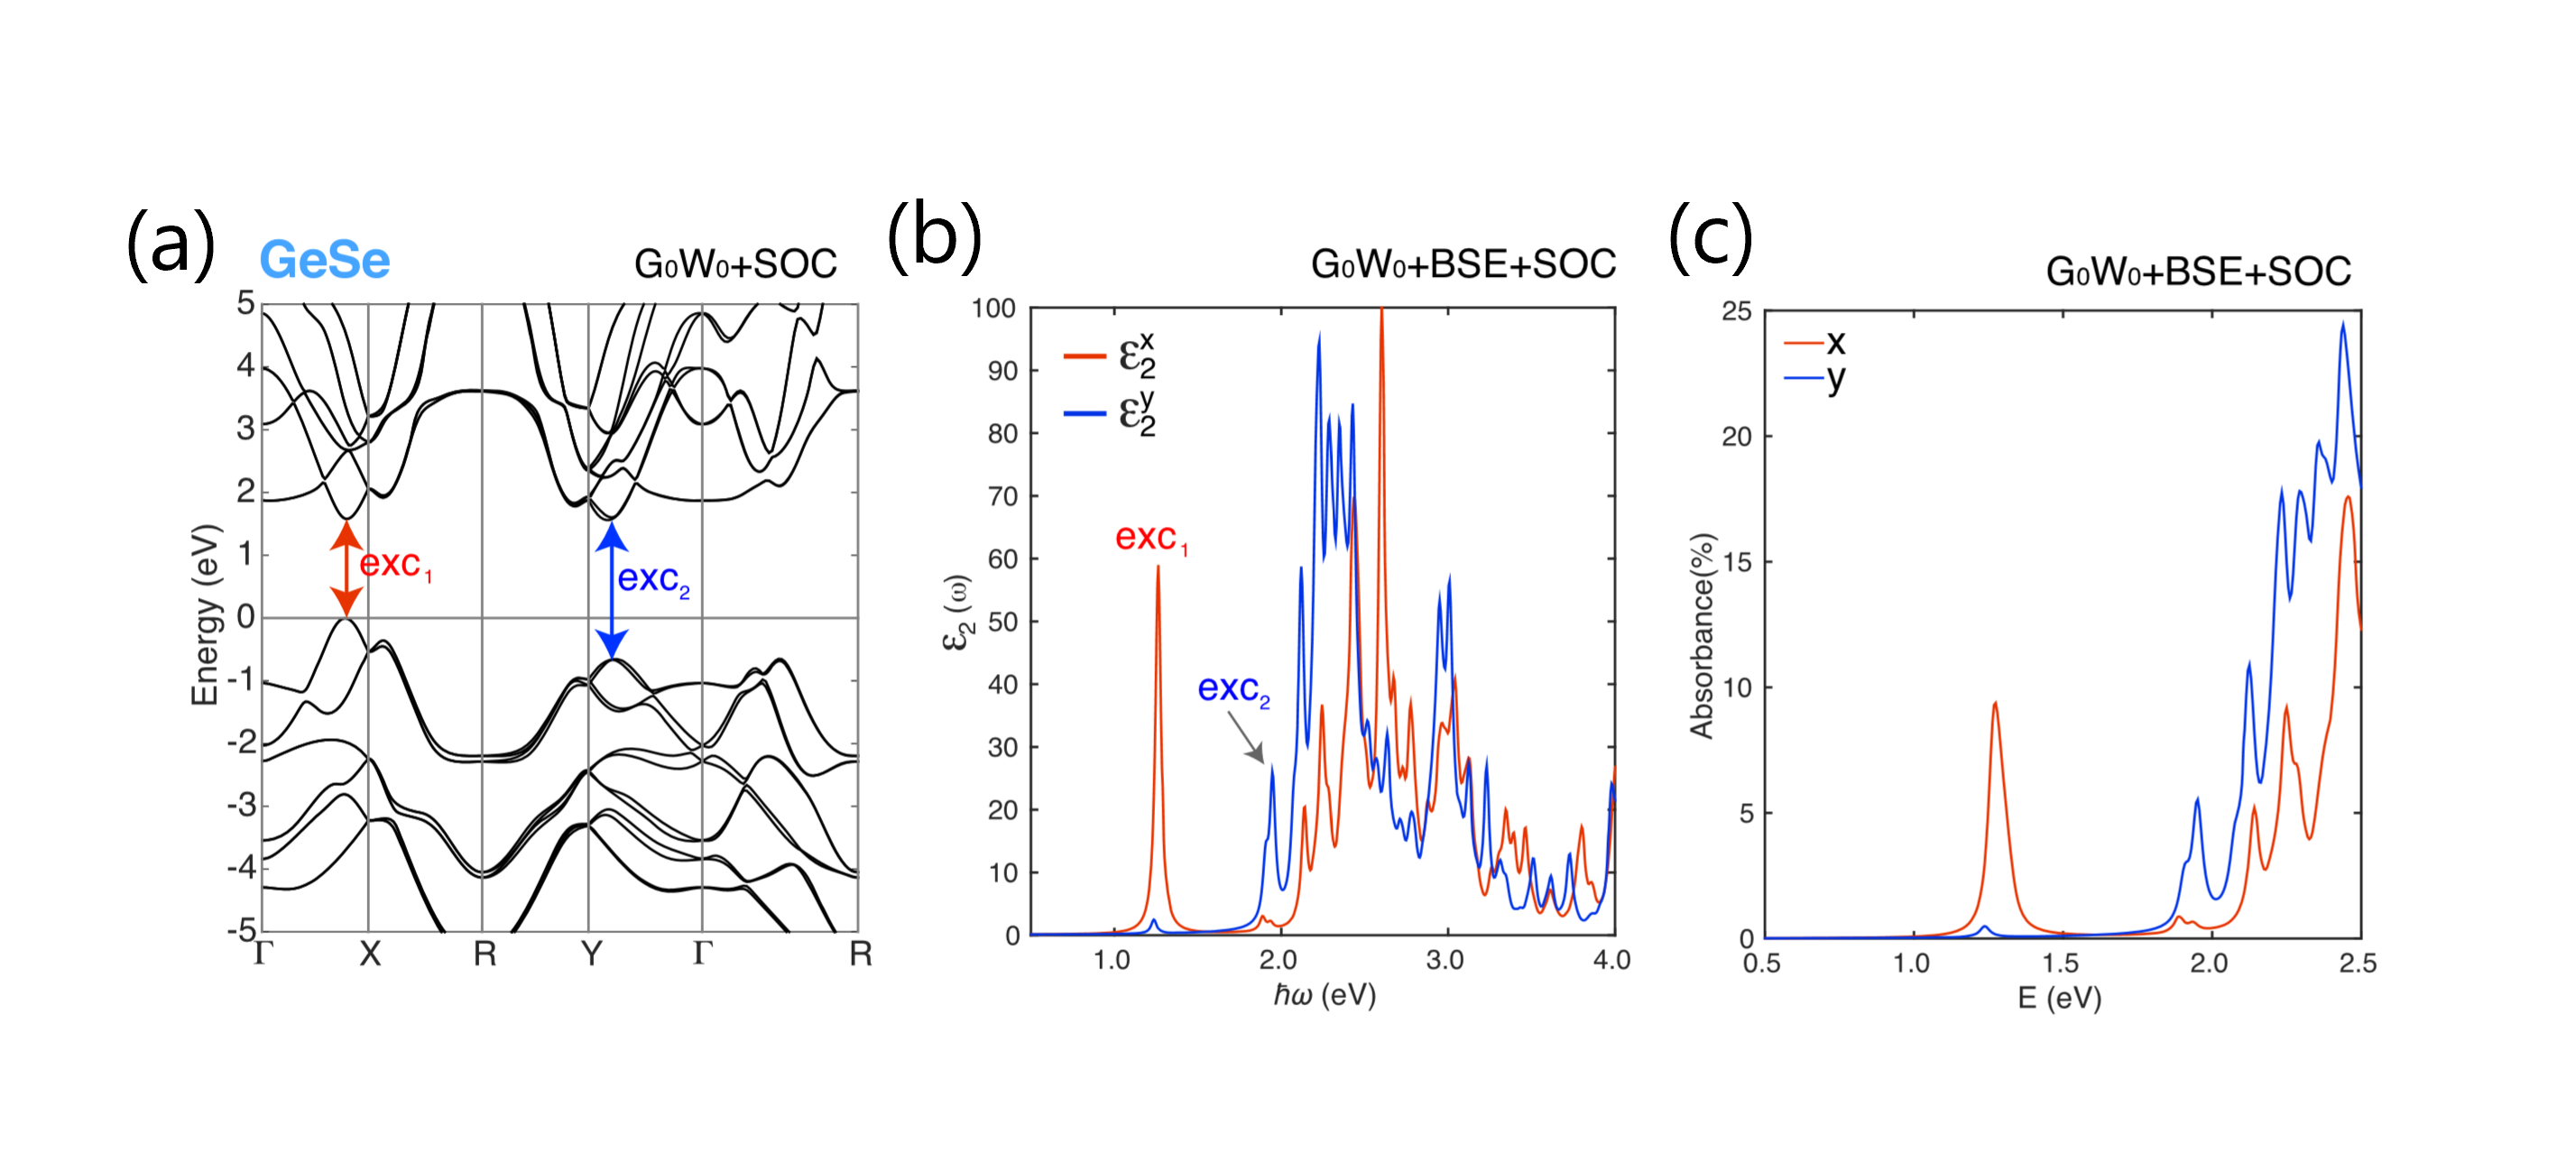
\includegraphics[width=0.8\textwidth]{./pic/019.png}
\caption{(a)在$G_{0}W_{0}$近似下得到的GeSn能带图,从图中可以看到二维层状GeSn是一种半导体,结构上的各向异性导致其对光的相应也具有各向异性(b)通过能带计算出的介电常数,有着明显的各向异性(c)单层GeSn的光吸收度}

\label{dog019}
\end{figure}

\section{双金属三卤化物}
对于铁电性与铁磁性的多铁材料,其多铁性的研究核心是在铁电性与铁磁性的耦合。二维双金属三卤化物是一种新型通过理论计算发现的二维多铁材料。$ReWCl_{6}$是一种单相同时具有铁磁性与铁电性的第一类二维多铁材料。\cite{xu2020electrical}由于铁磁性与铁电性来源不同,第一类多铁材料与第二类相比电磁耦合要弱。这种材料具有面内的电极化与铁磁性和反铁磁性两种磁性状态,而且通过外加电场同时改变电极化方向与两种铁磁相之间的切换。是一种可以通过电场控制磁场的二维多铁材料。

\subsection{结构与铁电性}

\begin{figure}[h]
    \centering
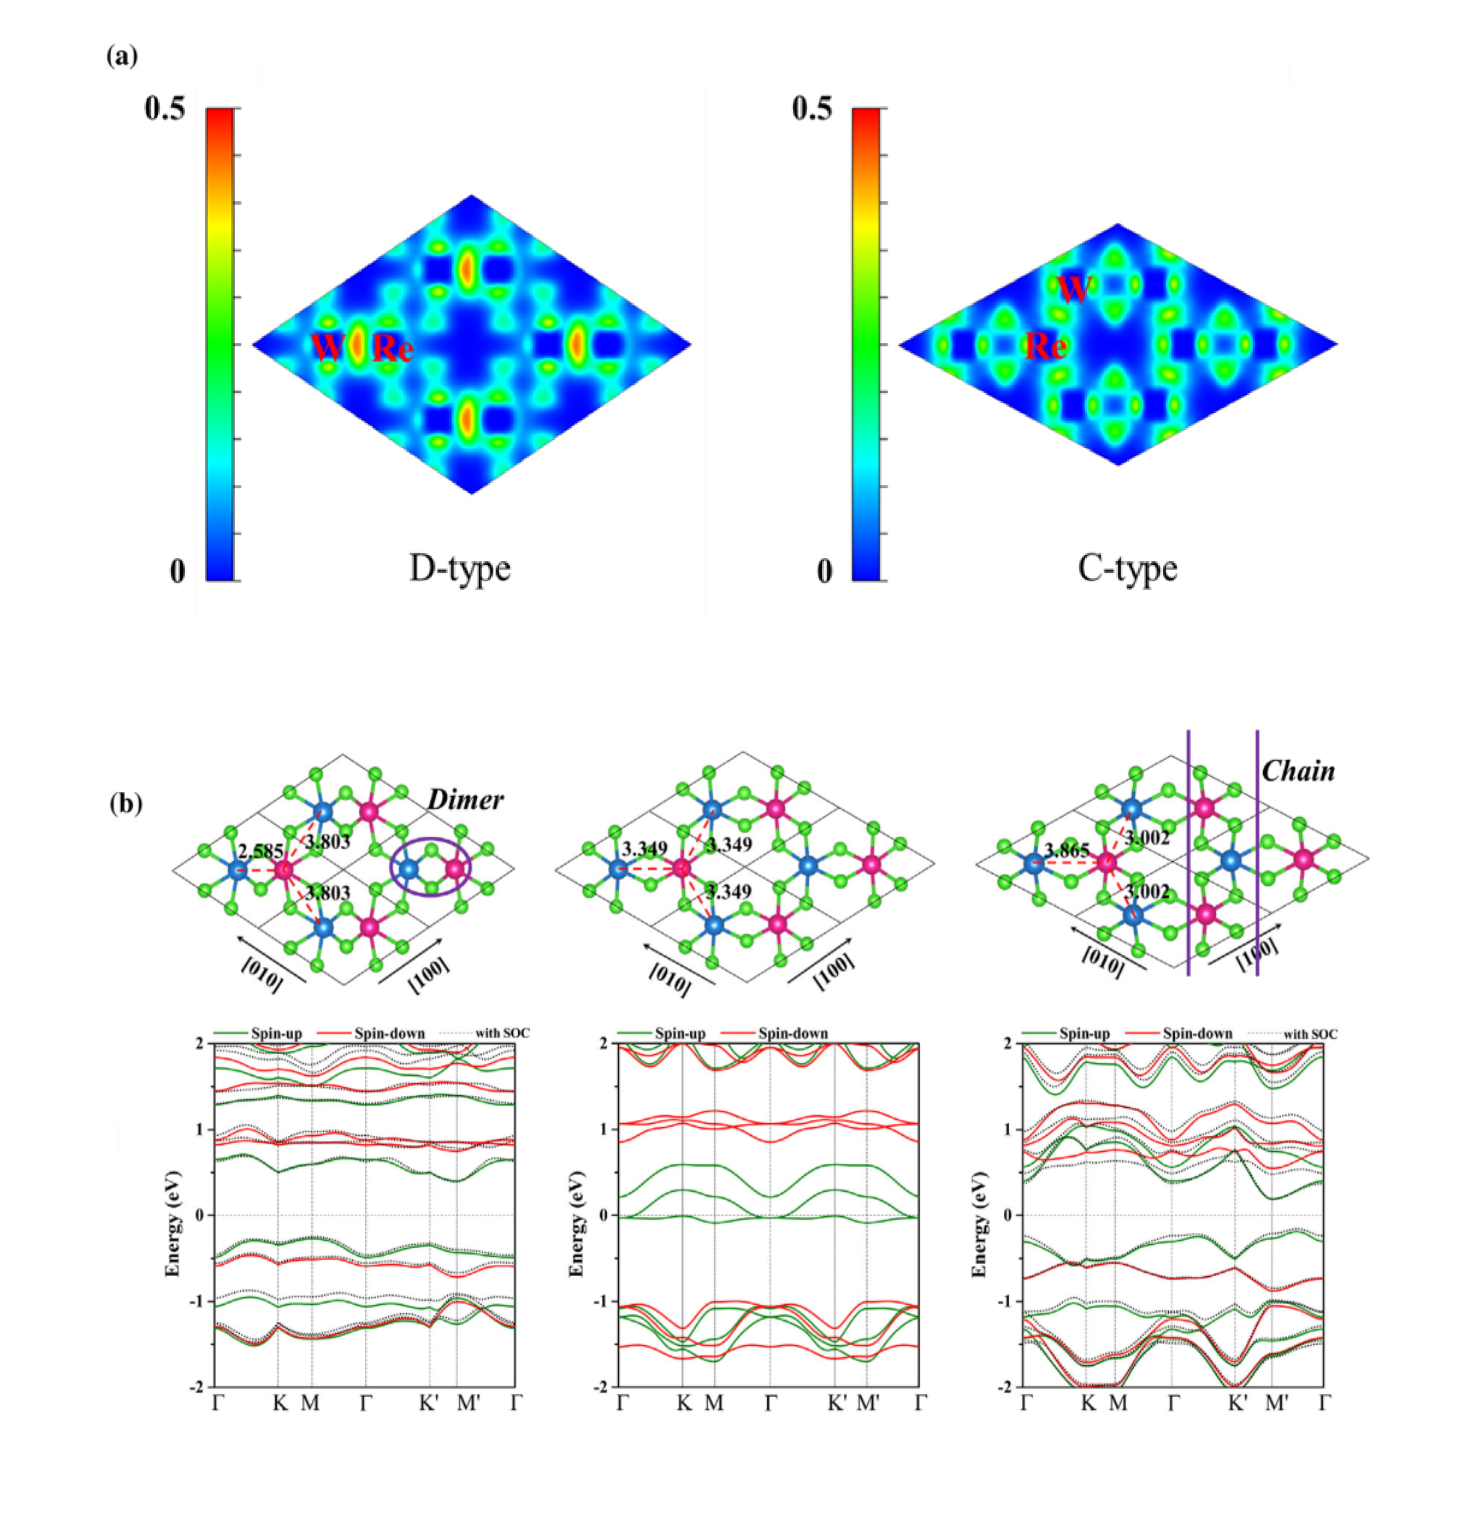
\includegraphics[width=0.8\textwidth]{./pic/021.png}
\caption{(a)D型和C型电子分布图\ 从图中可以明显看出两种结构的电极化方向、强度不同\ (b)$ReWCl_{6}$三种结构(D型、C型与高对称的$C_{3}$型)的俯视图与能带结构 \ 其中蓝色代表W原子、红色代表Re原子、绿色代表氯原子,层状结构之中的W-Re聚合体与W-Re-W-Re链条已被标出。从三种不同结构的能带图上可以看出,D型、C型均是有着不同带隙的半导体,高对称的$C_{3}$型是导体。通过虚线所示的考虑自旋轨道耦合后的两种计算结果后的差别,自旋轨道耦合对体系的影响不大,不是影响$ReWCl_{6}$多铁性性质的决定性因素。}

\label{dog021}
\end{figure}

与之前提到的过渡金属卤化物类似,二维双金属卤化物层状结构也是类似的三角形结构。对于三角形结构,一般有$C_{2}\text{、}C_{3}$两种对称性。铁电性的出现通常意味着空间对称轴的破坏与对称性的降低。对于二维晶体结构,对称性的降低通常是由于某些原因$C_{3}$对称性不复存在,这样在$C_{2}$对称轴这个方向就会成为一个特殊方向,这个特殊的方向往往就是电极化的方向。如图所示,原子位移与结构扭曲导致$ReWCl_{6}$的对称性被破坏,由$C_{3}$高对称状态转化为两种$C_{2}$低对称状态,分别为D型与C型。D型C型两种结构由于原子移位不同,产生两种相反的自发极化方向。这两种类型的微观结构不同,其表现出来电磁性质也不同。因此在通过外加电场对这两种铁电状态进行反转时,其磁性性质也会随之改变,可以通过外加电场的方式改变$ReWCl_{6}$的磁性质。

\begin{figure}[h]
    \centering
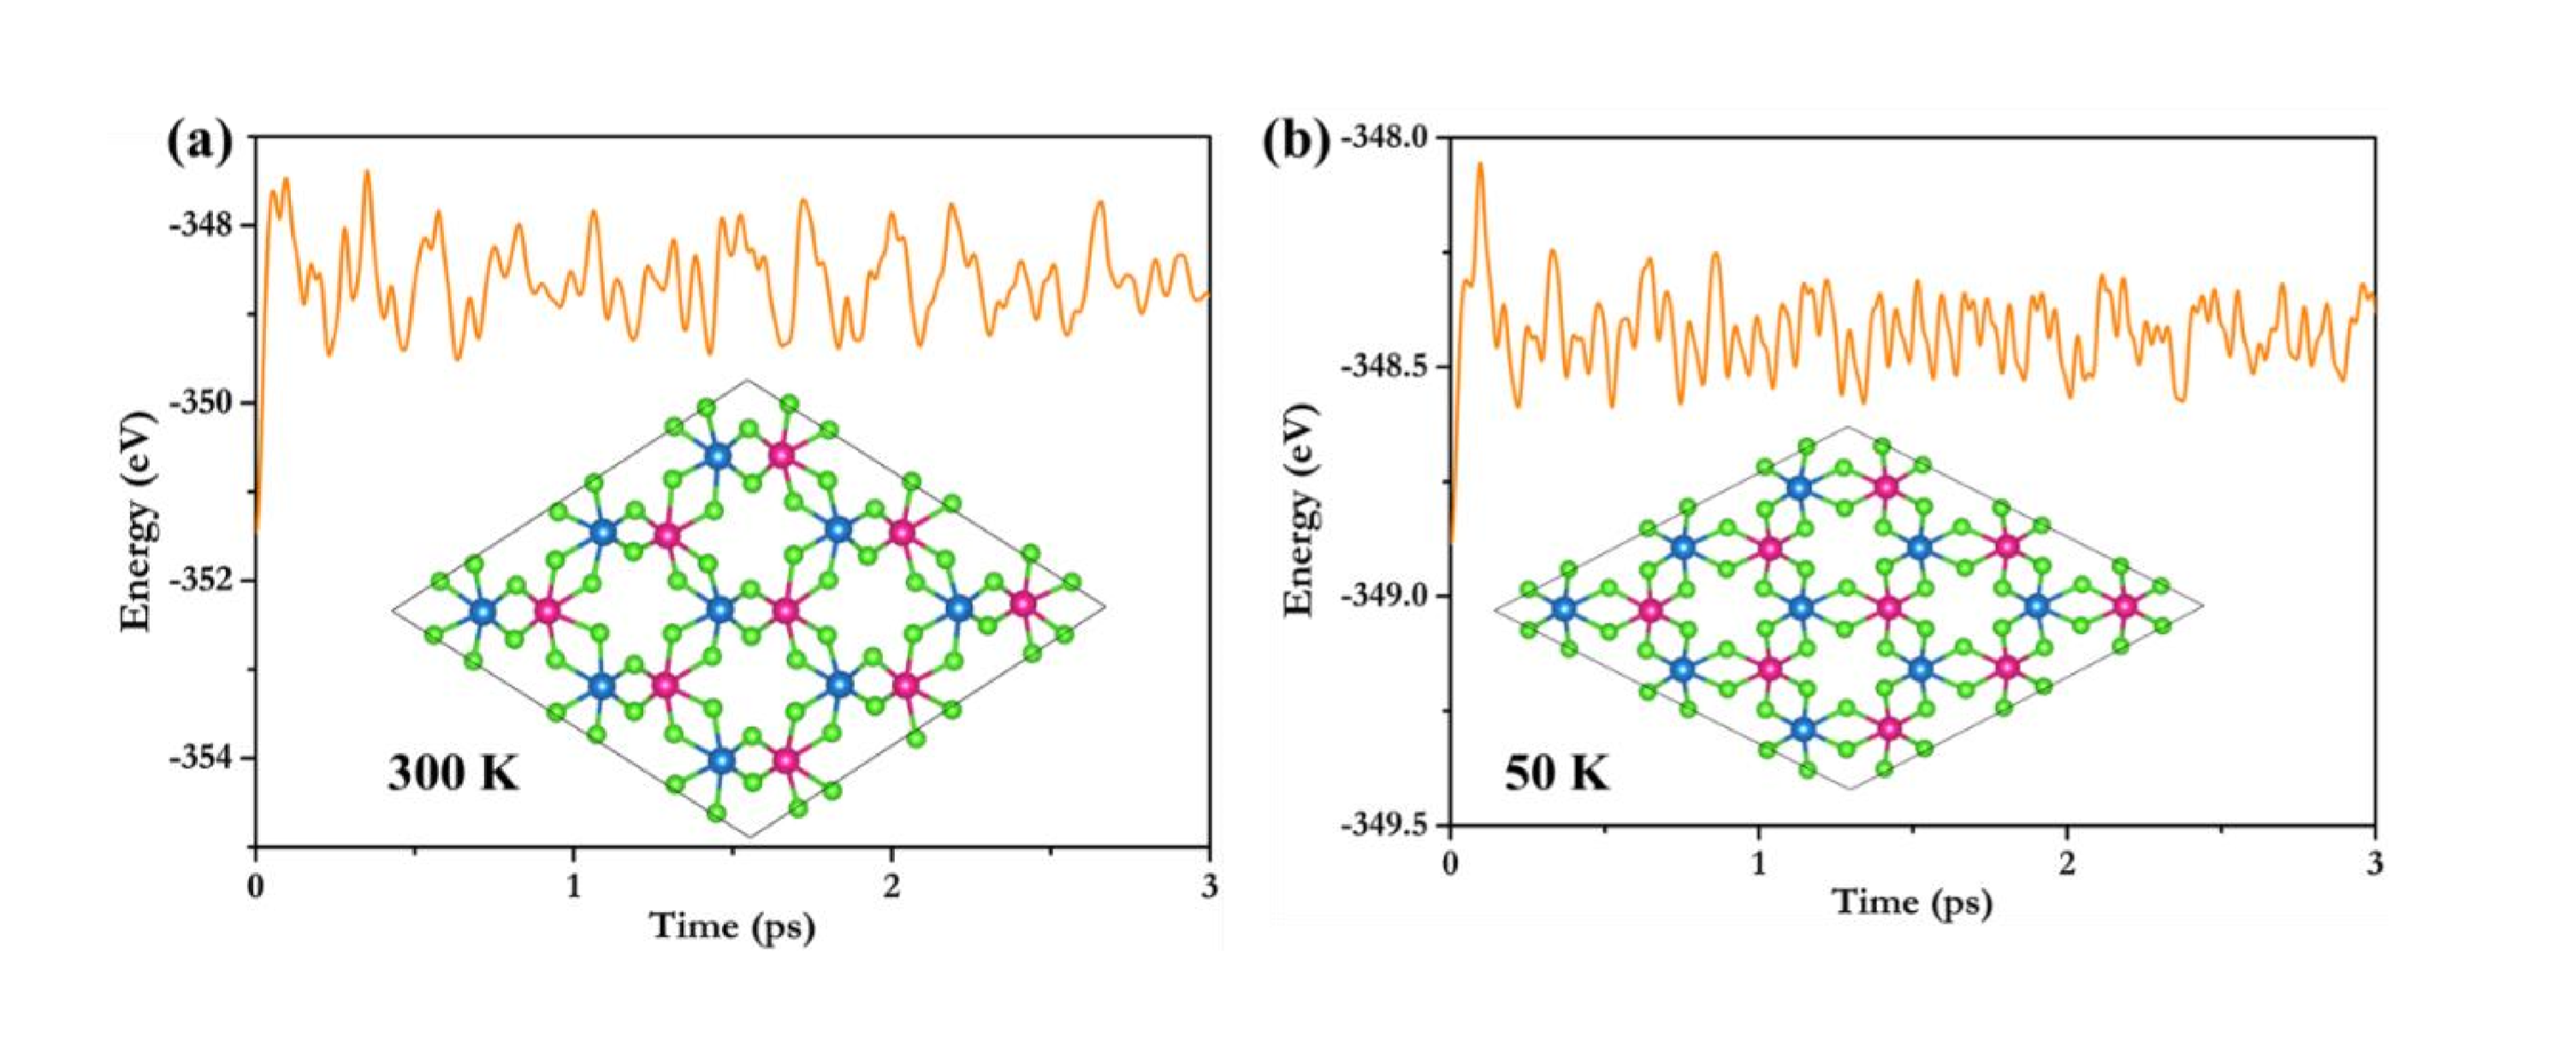
\includegraphics[width=0.8\textwidth]{./pic/020.png}
\caption{基于牛顿力学的分子动力学模拟\ 通过对D型与C型AIMD模拟,观察其总能量的波动。结果表明,D型结构在300K与C型在50K下是稳定的,在超过100K的情况下,C型总会自发向D型转变}

\label{dog020}
\end{figure}

通过第一性原理计算,$D_{3}-ReWCl_{6}$是没有带隙的导体,而两种具有铁电性的D型与C型则是具有0.67eV、0.38eV的半导体。而整个系统中的自旋轨道耦合几乎不会影响电子结构。\cite{ISI:A1993KJ51800070}

\begin{figure}[h]
    \centering
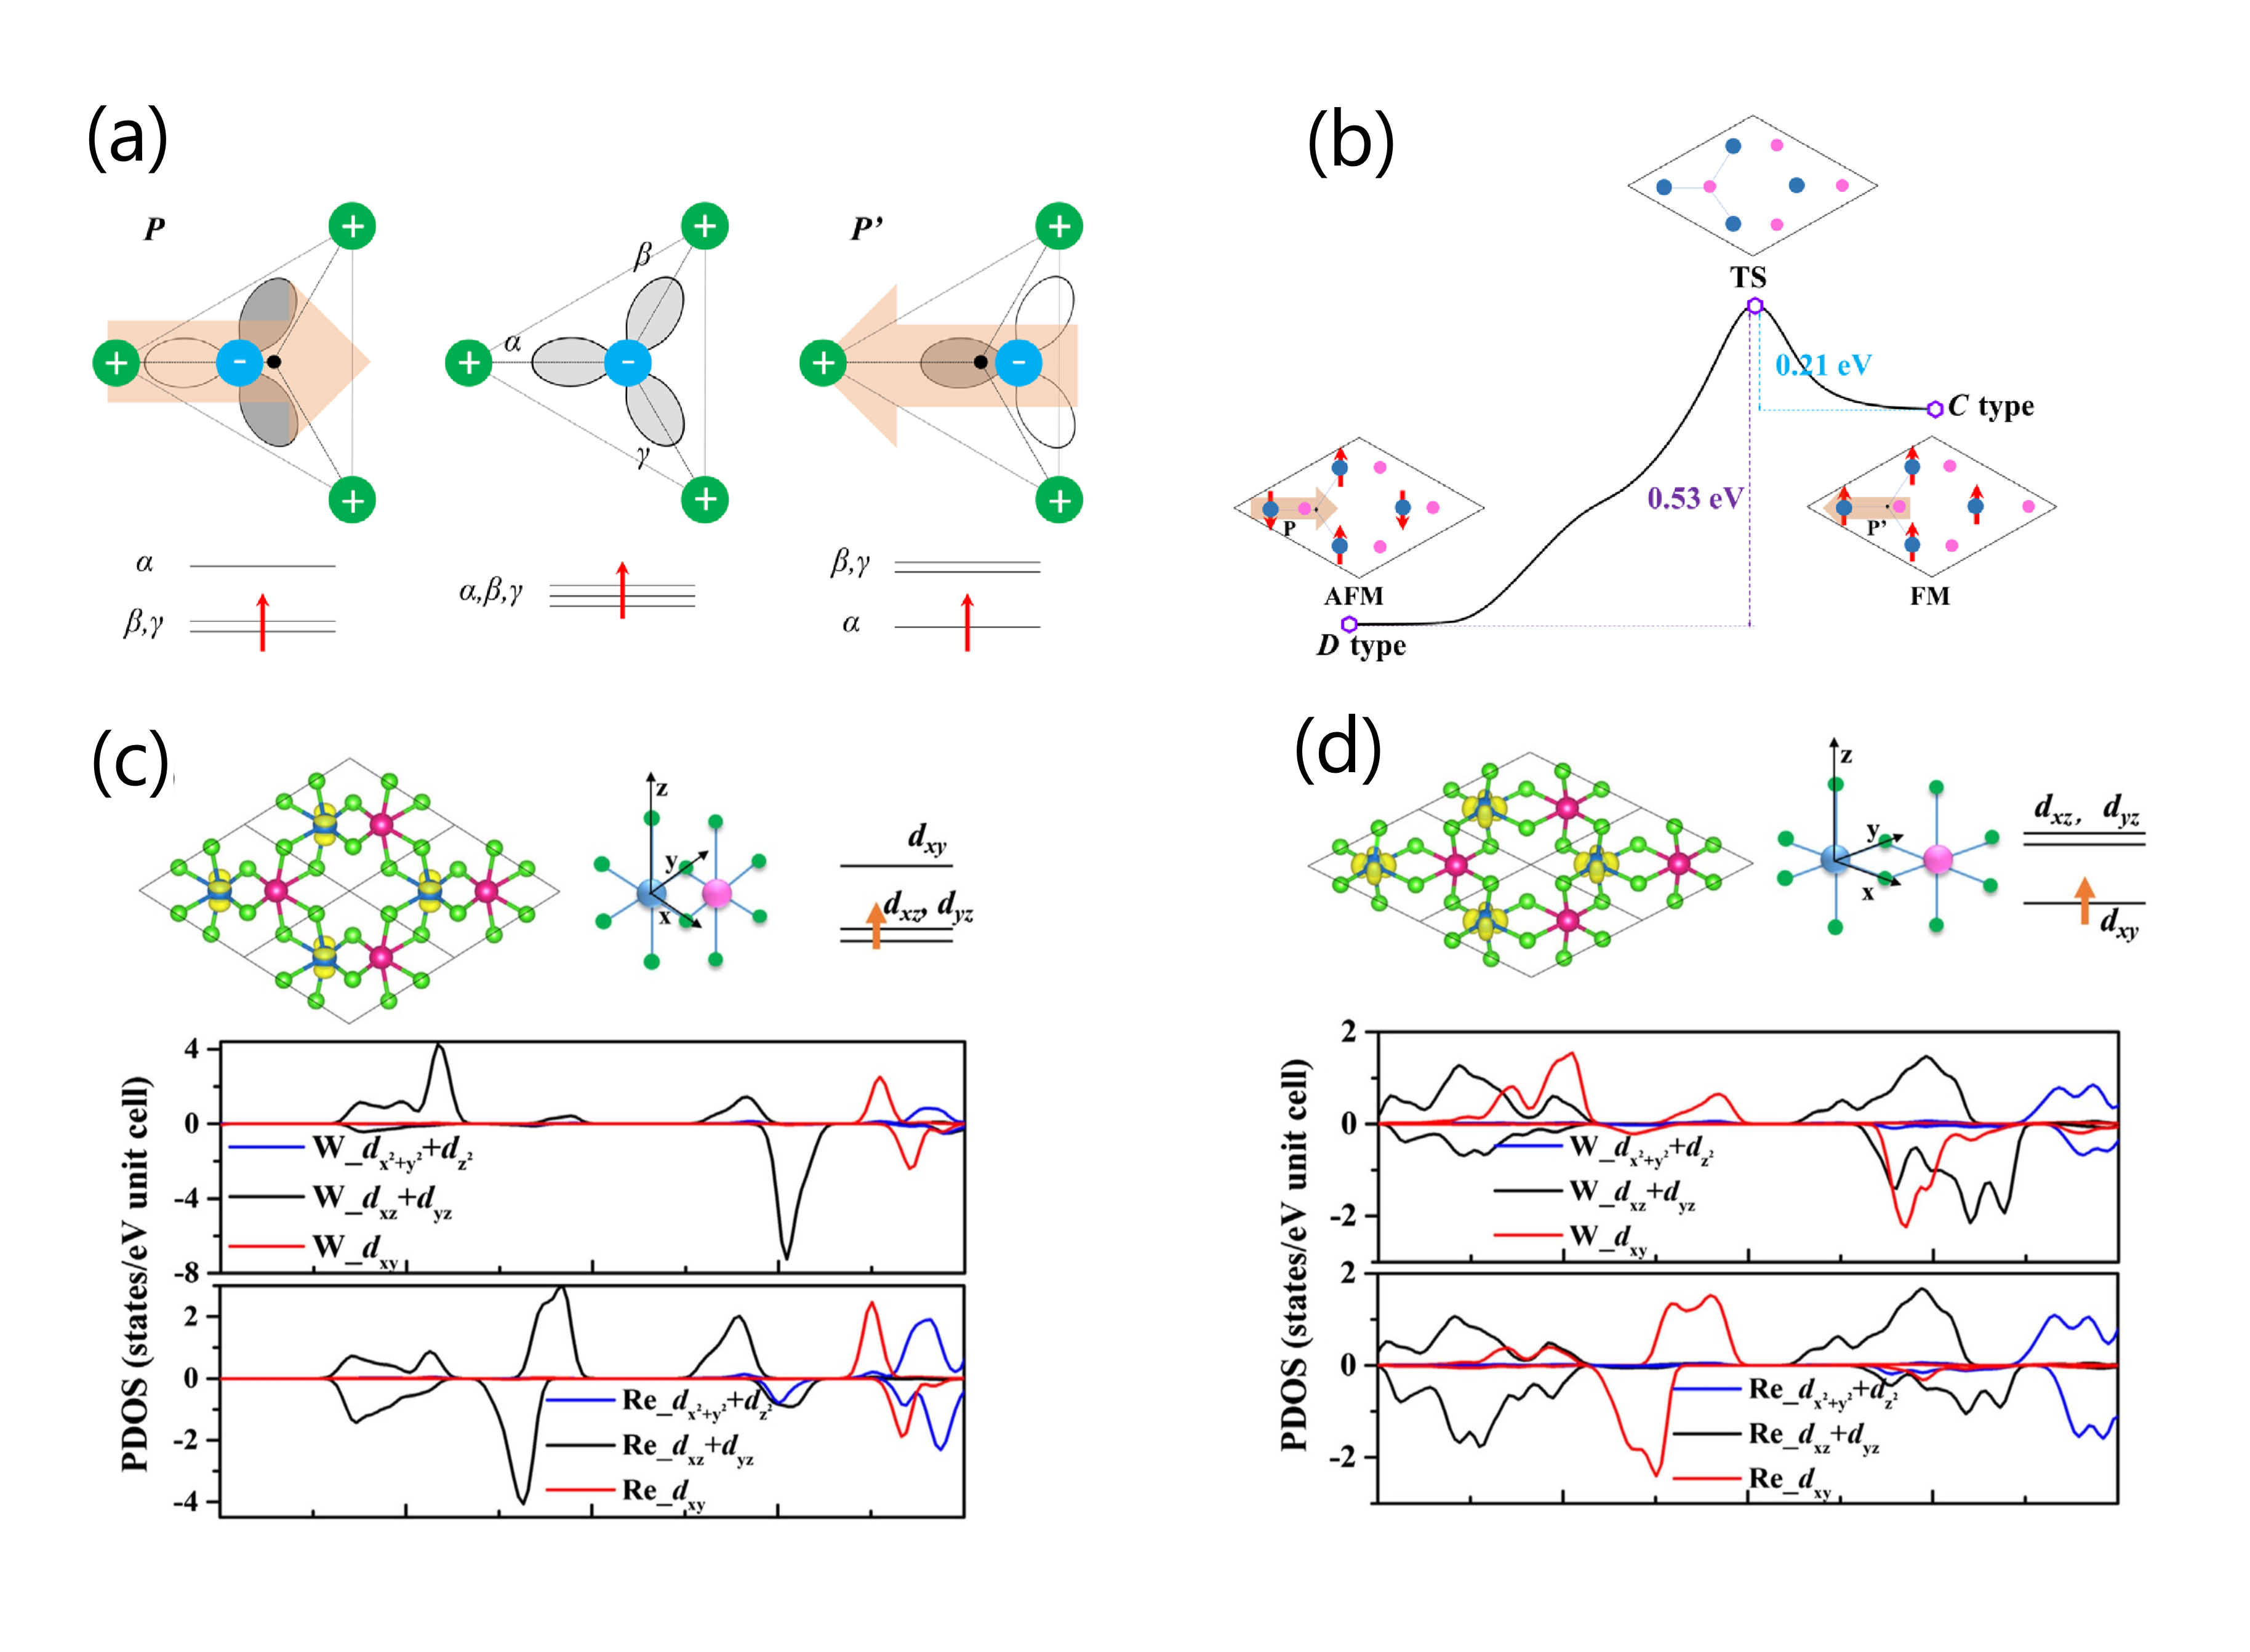
\includegraphics[width=0.8\textwidth]{./pic/022.png}
\caption{(a)$ReWCl_{6}$的D型、C型和高对称性$C_{3}$型的示意图\ 图中绿色与蓝色分别代表带电的正负离子,从图中可以看到高对称性$C_{3}$型仍然存在中心对称轴,在面内没有自发极化,相应的,电子能级结构也没有出现不对称的分离与能量变化,D型、C型结构中心金属阳离子发生了位置偏移,导致中心对称性消失,D型、C型两种铁电相位于三角形中心的阳离子偏移方向不同,所导致的这两种类型的自发极化方向相反,同样的,金属阳离子周边的电子运动所受到阴离子影响也会发生变化,这导致了D型、C型电子能级发生分裂与变化。(b)D型、C型两种铁电相之间的相变过程的动力学路径。蓝色代表W原子,红色代表Re原子,Cl原子被忽略,上下箭头代表自旋方向。在D型、C型两种铁电相之间有一个转化中间态势垒,D型的能量要高于C型,在发生两种铁电相变时,不仅仅自发极化方向会反转,系统的磁性质也会从反铁磁性与铁磁性之间转化。(c)(d)D型、C型两种的电子自旋态密度,两种不同类型$W_{t2g}$轨道不同占据情况。}

\label{dog022}
\end{figure}

受制于晶体的三角形结构,面内的电极化方向是收到限制的,两种铁电相D型和C型的电极化方向可以进行间隔120°的旋转,如果进行180°的反转,即进行电极化的反转,只能通过C型和D型之间的相变或者进行对整个结构的60°旋转。这一点可以通过在面内加入静电场来确认。与传统的二维铁电材料不同,二维$ReWCl_{6}$在发生电极化方向的反转时,会经历一个D型、C型之间的相变,在这种情形下,在自发极化方向反转的时候,电极化的变化不是连续的,中间有一个突变的过程,这种突变过程比正常的量子极化效应要大的多,突变来自于D型和C型,高自旋和低自旋状态之间的相变。\cite{WANG20122063}

\subsection{铁磁性}

根据Re元素和W的化合价,系统的铁磁性来源于$W^{5+}-d^{1}$的一个未成对电子贡献出的1$\mu_{B}$磁矩。而$Re^{+}-d^{6}$电子完全占据了$Re-t_{2g}$轨道,通过应用MLWFs方法对电子轨道能量进行分析,D型结构与C型结构自旋极化的电子结构不同。在C型中,由于$d_{xz}\text{和}d_{yz}$能量比较高,自旋磁矩电子主要占据$d_{xy}$轨道,在C型结构中自旋磁矩电子占据在$d_{xz}\text{和}d_{yz}$轨道。自旋哈密顿量可以写成:
\begin{equation}
    \hat{H}=-\sum_{i}(2J_{1}\vec{S}_{i}\cdot \vec{S}_{i,1}+ J_{2}\vec{S}_{i}\cdot \vec{S}_{i,2})
    \label{zixuan}
\end{equation}
其中$J_{1}\text{和}J_{2}$分别是在[1\ 0\ 0][0\ 1\ 0]方向和[1\ 1\ 0]方向上的交换积分。通过计算可得D型的$J_{1}\text{和}J_{2}$分别是2.00meV和−1.00meV,正负号表示反铁磁耦合与铁磁耦合,D型的基态是反铁磁性的。C型的$J_{1}\text{和}J_{2}$分别是-1.75meV和0.75meV ,基态是铁磁性的。\cite{PhysRevB.82.094116} 这个结果可以这样理解,反铁磁性的5d轨道交换积分与W之间的距离有关,短的W-W间距会增强反铁磁性,长的W-W距离会增强铁磁性,两种类行不同的W-W距离导致了铁磁性与反铁磁性的不同。蒙特卡洛模拟显示D型和C型的磁性临界温度在21K和10K左右。\cite{katsura2005spin}

\begin{figure}[h]
    \centering
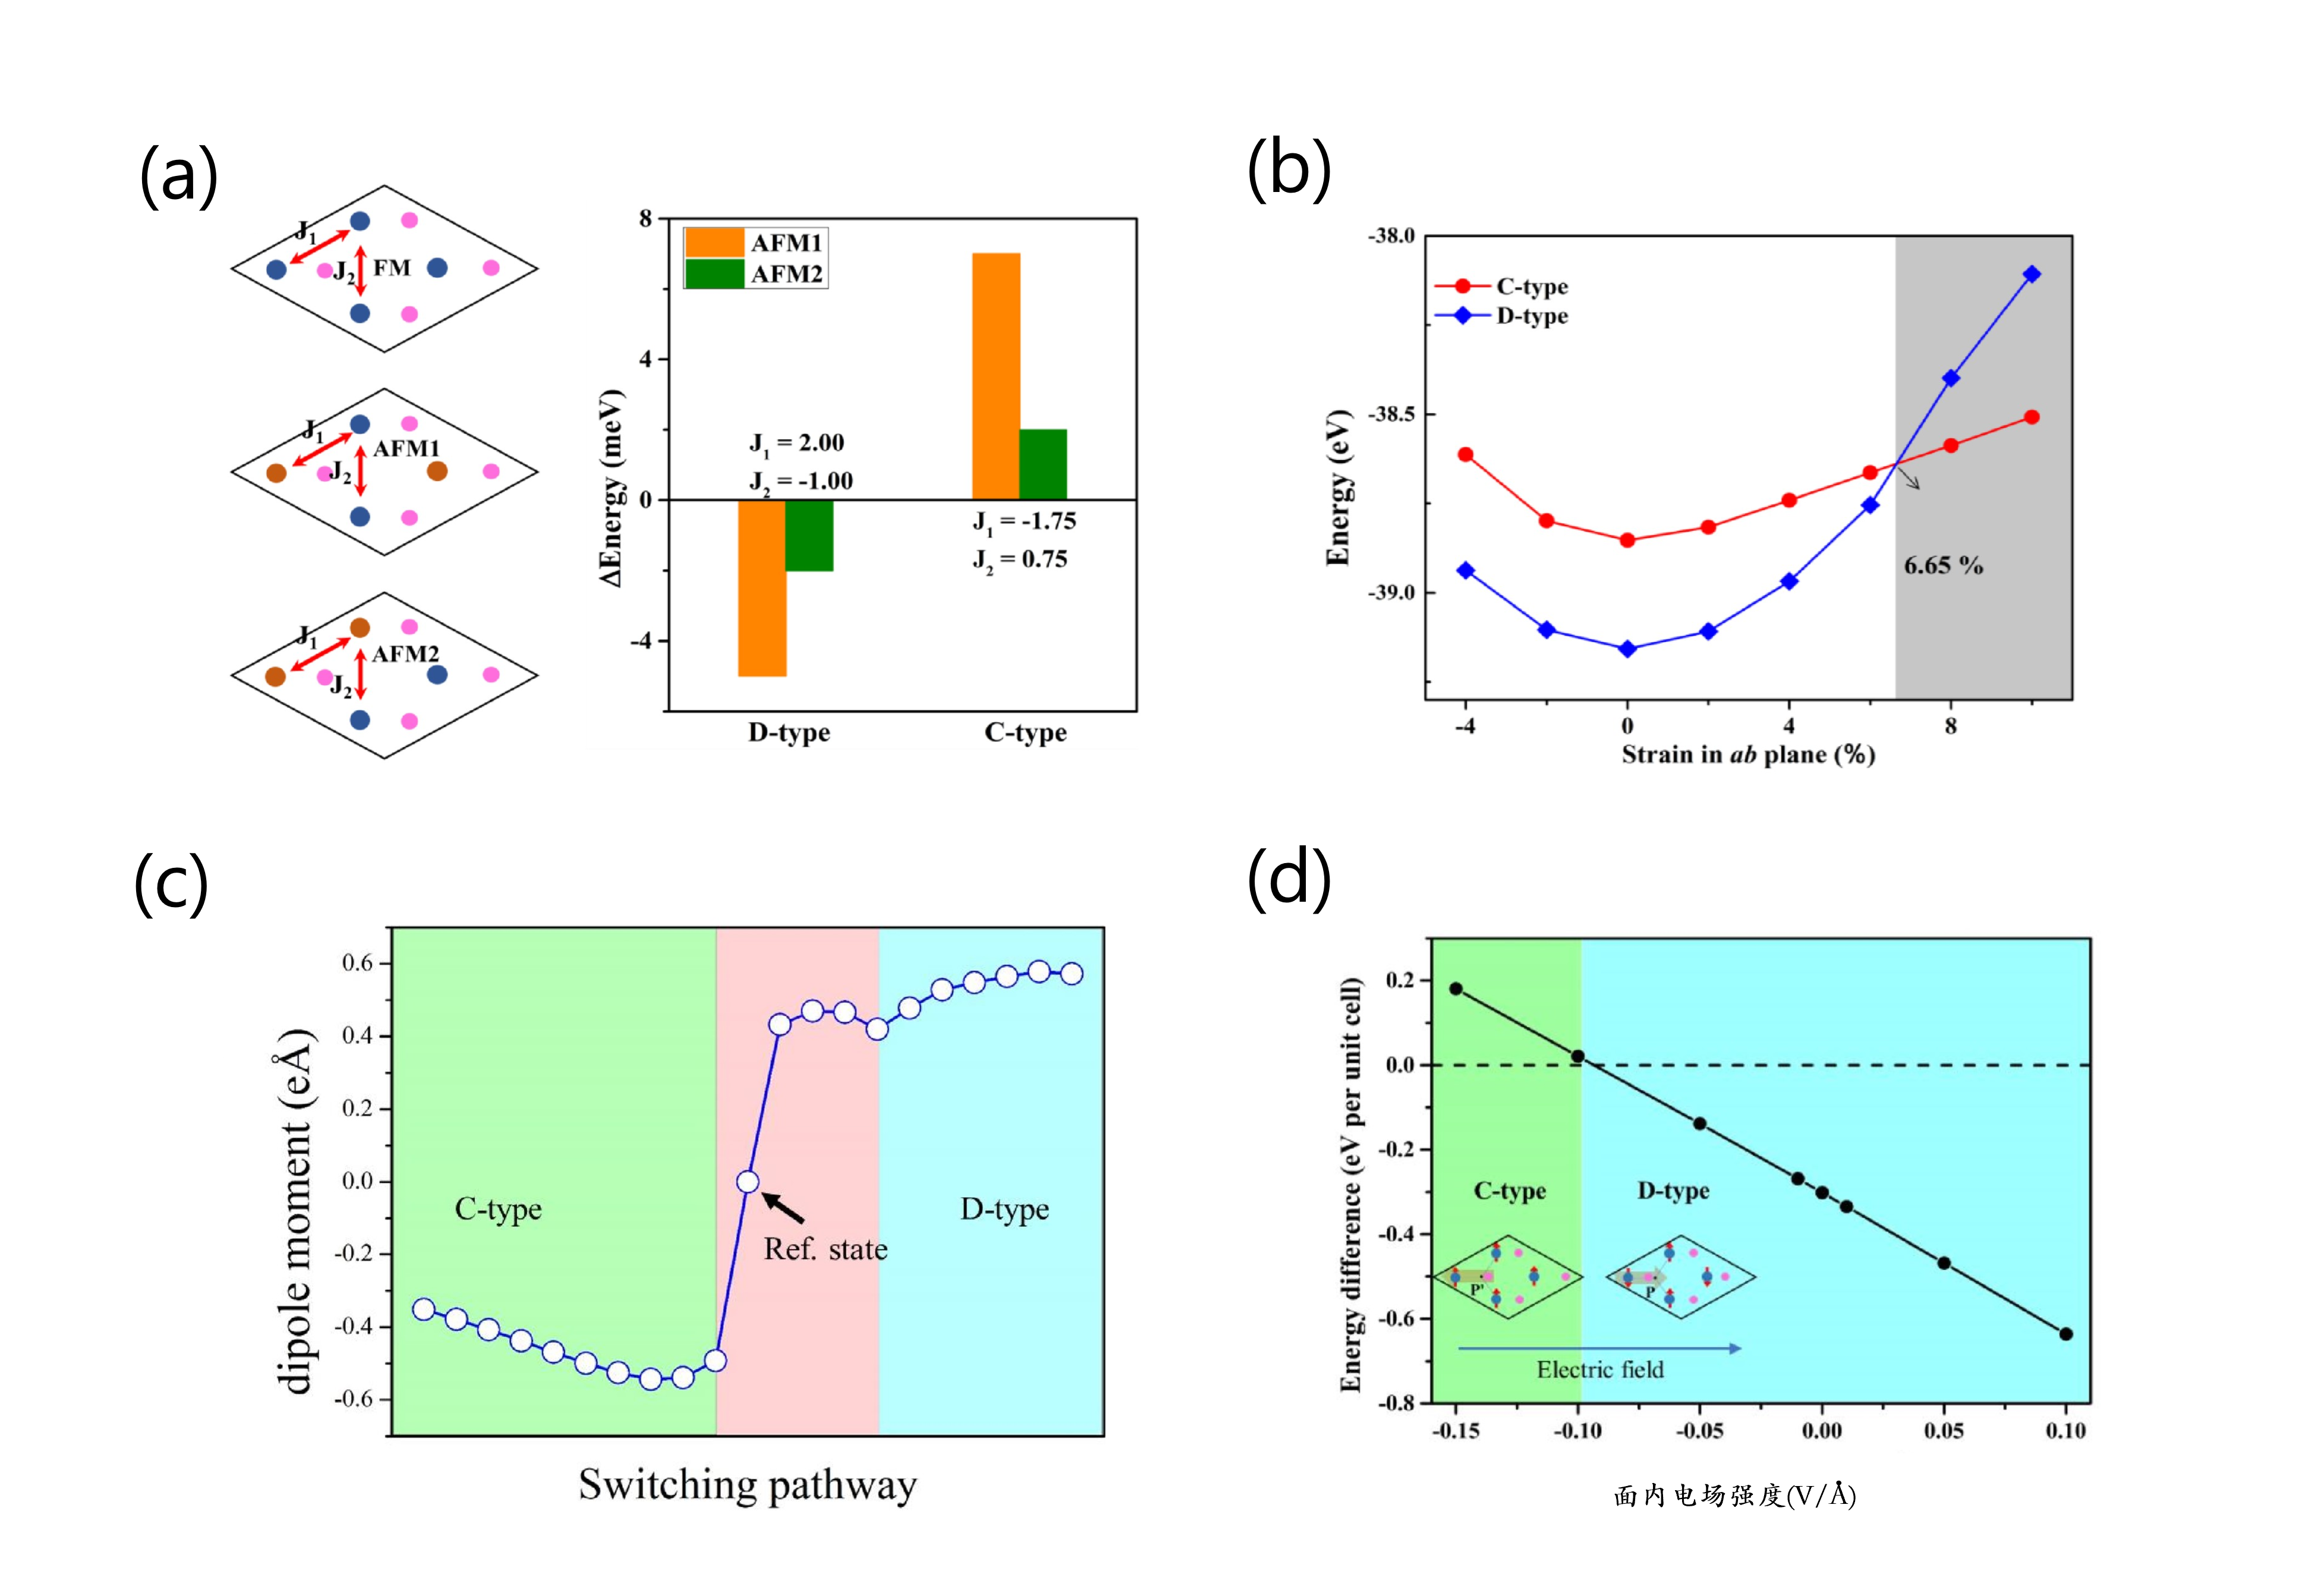
\includegraphics[width=0.8\textwidth]{./pic/023.png}
\caption{(a)$ReWCl_{6}$可能的几种磁矩排布方式,由两种反铁磁相和一种铁磁相,大实心圆表示W原子,小实心圆表示Re原子,深蓝色和橙色分别是向上自旋和下自旋状态,$J_{1}\text{和}J_{2}$分别是在[1\ 0\ 0][0\ 1\ 0]方向和[1\ 1\ 0]方向上的交换积分。右边是不同磁矩排布方式在不同类型下的交换积分和总能量,正负号表示反铁磁耦合与铁磁耦合,反铁磁的D型AFM1状态的能量最低。(b)双轴应变对D型与C型两种类型总能量的影响,在没有应变时D型的能量更低,在应变大于6.65\%时,C型的能量更低。\cite{ISI:000480497100035} 这表明在适当应变的条件下,也可以实现D型与C型两种类型的转换。(c)D型与C型之间转换时电偶极矩的变化。与一般铁电材料电极化的连续变化不同,$ReWCl_{6}$电极化方向反转时存在着一个突变过程,涉及到D型与C型之间的相变,转化中间存在着一个类似高对称性$C_{3}$型的没有电极化的状态。(d)在施加面内电场时D型与C型能量差的变化,电场的正负号分别表示沿[1\ -1\ 0]和[-1\ 1\ 0]方向的电场。沿[-1\ 1\ 0]方向足够大的面内电场可能会导致从D型过渡到C型,从而导致电极化的反转。}

\label{dog023}
\end{figure}

\subsection{电磁耦合}

作为一种第一类的二维多铁材料,通过常规的通常的电磁耦合方式的作用是微弱的,然而$ReWCl_{6}$的D型与C型两种状态电极化方向相反,铁磁性也不同,这在另一种层面上实现的电磁耦合。经过计算,$ReWCl_{6}$的电磁耦合强度可以达到$Fe/BaTiO_{3}$的水平。D型与C型两种状态的能带带隙也不同,D型与C型两种状态可以用外加电场的方式进行转化,这同样可以意味着可以通过外加电场调控电子结构。与常规的多铁材料的电磁耦合中磁化强度会随着外加电场变化不同,当施加的电场大于矫顽场时,极化方向会反转,磁相会同时改变,$ReWCl_{6}$的磁场强度并不会随着外加电场的增大而增大,因为在完成铁磁相与反铁磁相的切换之后没有明显的机制支持铁电性与铁磁性的强耦合。一般的多铁材料电磁耦合系数$\alpha=\mu_{0}|\Delta\bm{M}|/E$,但在$ReWCl_{6}$情况下这样的表述形式需要进行重新解释以适应$ReWCl_{6}$独特的电磁耦合方式。如果用铁磁相与反铁磁相转化时的$\Delta\bm{M}\text{和}E$,$\Delta\bm{M}$为改变极化方向前后的磁化强度变化,E为矫顽电场,进行计算,可以得出~666G(原文如此)的结果,比$Fe/BaTiO_{3}$的~120G大得多。

作为与铁电性关系更加密切的铁弹性,对二维$ReWCl_{6}$,在平面内部施加合适的应变也会导致D型与C型两种状态相互转化。\cite{ISI:000274700900024}



总的来说,$ReWCl_{6}$是一种新型的二维多铁材料。$ReWCl_{6}$通过一种特殊的铁电相与晶格结构耦合,进一步影响铁磁性的方式实现了铁电性铁磁性不同源的第一类多铁材料的强铁电铁磁耦合。通过施加合适的外电场实现面内电极化的反转与铁磁相与反铁磁相的转化,这些发现揭示了二维多铁性材料中磁相变电学控制的磁电耦合新机理,这很可能引起自旋电子学的研究和应用。从另一方面,$ReWCl_{6}$多铁性与电磁耦合产生的机制并不能支持通过磁场控制电极化或者是进行不同的铁磁性之间的转化,从这个角度看来,$ReWCl_{6}$的多铁性是不全面的,在将来的应用方面也许会受到一定的限制。
\chapter{多铁材料的设计与理论工具}

\section{多铁材料研究之中的基本方法}

随着对多铁材料研究的进一步深入,越来越多的新的实验、理论方法涌现出来。在实验手段方面,观测设备愈发先进,实验性的电子探针,可以探测电荷的自旋轨道自由度,探测的空间分辨率已经到达元胞尺度,时间分辨率已经达到次飞秒的量级,接近交换作用的时间尺度。激光脉冲沉积也有很大的进展。在理论工具方面,密度泛函理论依然解释多铁性质与预测新的多铁材料的黄金方法\cite{zhong1994phase},在大型系统中第二性原理越来越有价值。基于分子动力学的模拟,如果模型选择合适,其结果完全可以拟合DFT计算的结果。
\begin{figure}[h]
    \centering
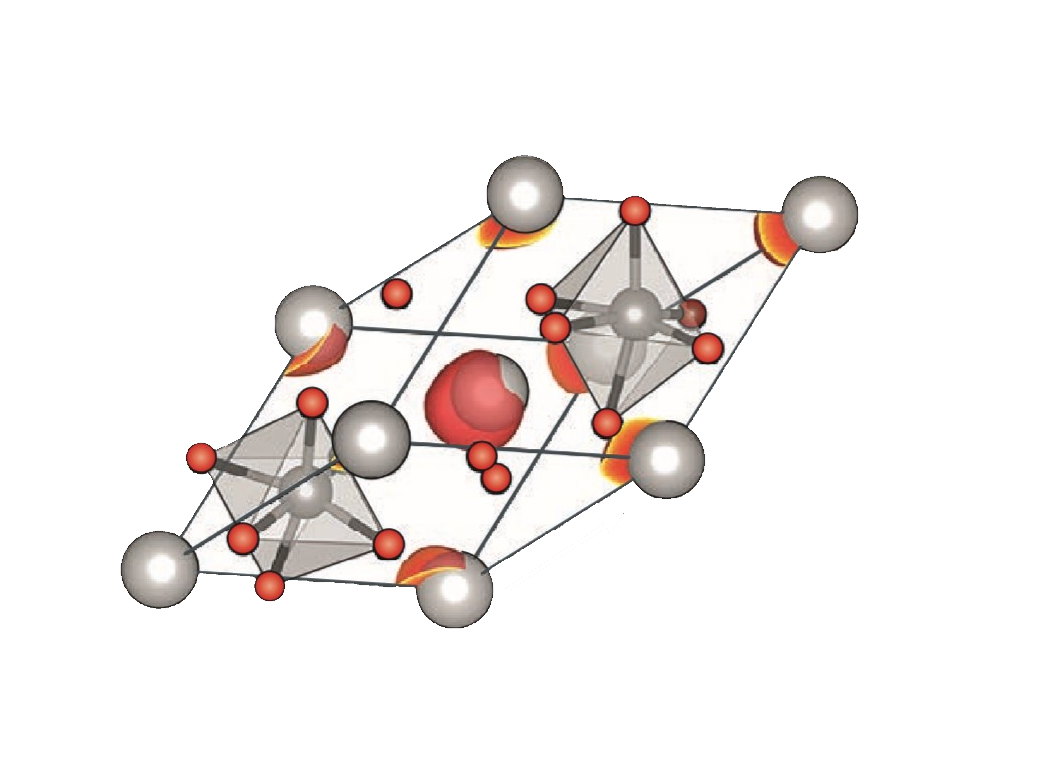
\includegraphics[width=0.8\textwidth]{./pic/007-2.png}
\caption{$BiFeO_{3}$晶体结构}
\label{dog007}
\end{figure}

\section{材料理论设计的基本原理}

结构决定性质,良好的物理性质的背后离不开与之相适应的结构。多年以来的研究成果告诉我们,分子、原子、原子核和电子的运动结构规律的研究离不开量子力学。实验已经证明,量子力学在微观低速领域是正确的,能够对物理现象进行良好的描述以及预测。一般认为,量子力学有着四个基本假定。
\paragraph{第一个假定:}微观粒子的运动状态可以用波函数来描述。
\paragraph{第二个假定:}每个可观测的力学量$\bm{F}$都有一个厄密算符$\bm{\hat{F}} $相对应,力学量的取值只可能是所对应算符的本征值。
\paragraph{第三个假定:}当在一定的运动状态之中测量某力学量$\bm{F}$时,可能得到不同数值,其平均值$\langle \bm{F} \rangle$按照以下公式计算:
\begin{equation}
    \label{eq1}
    \langle F \rangle = \frac{\int \Psi^{*} \hat{F}\Psi d \tau}{\int \Psi^{*} \Psi d \tau}
\end{equation}
\paragraph{第四个假定:}微观粒子的运动方程由薛定谔方程描述
\begin{equation}
    \label{eq2}
    \frac{\partial \Psi}{\partial t}= \frac{i}{\hbar} \hat{H} \Psi
\end{equation}
以上的四个基本假设没有涉及到相对论效应,适用范围为微观低速情况下。

对于宏观物质,尤其是具有$\bm{N_{A}}$量级的原子的物质,这种多粒子系统很难直接应用薛定谔方程直接得到微观粒子的波函数,对于周期性结构的晶体需要采取一些近似手段来大大减少计算量,晶体的空间周期性结构给简化计算工作带来了极大的方便,即使这样,除了少数特殊问题之外严格求解出解析解是不可能的的,通常只能采用数值计算的方法对问题进行理论研究。在进行数值计算时计算的方法可以分为两大类,从头计算和半经验计算。从头计算又叫第一性原理计算,采用真实的物理参数与哈密顿量,从支配客观世界的底层规律入手进行计算。半经验计算则是采用简化版本的哈密顿量,甚至采用基于牛顿力学的某些经验模型,通过实验的结果拟合参数进行计算。

原子中的原子核质量远大于核外电子,所以在研究晶体等周期性结构之中的电子运动时,通常认为原子核的位置是静止不动的,这样系统的波函数可以分解为只包含原子核坐标的$\bm{\Psi_{n}}$和只包含电子坐标的$\bm{\Psi_{e}}$两部分,这就是BO近似,是1927年波恩和奥本海默提出的。

对于单个的球对称原子,可以采用某些数学处理方法进行简化为径向方程求解,但对于多体问题,尤其时不存在球对称性的多体问题需要采取别的方法。量子力学的线性组合原理提供了一个良好的思路。电子的轨道波函数$\phi_{i}$可以表示为一系列的基函数$\eta_{j}$的线性组合。
\begin{equation}
    \label{eq3}
    \phi_{i} = \sum_{j} c_{ij} \eta_{j}
\end{equation}
其中$c_{ij}$为组合系数。如果系统内的任意波函数都可以表示为一组基函数的线性组合,这一组基函数可以称为完备的基组。在实际应用时,自然不可能将波函数展开到所有的基函数,只能选取有限多个基函数的组合来趋近于真实的波函数。如果将电子的波函数展开成有限个基函数的线性组合,对波函数的变分也就转化成为对若干系数的变分,这使得数值计算变得更加可能。

这些基函数的选取方式由很多种,在具有周期性结构的晶体或者有周期性边界条件时可以选取平面波作为基函数,在研究分子问题时可以采用原子轨道作为基函数。随着数值计算方法的发展,为了适应不同研究条件不同研究层次不同研究对象,人们提出了很多基函数。斯莱特型轨道(STO)是一种常用的基函数,基于对氢原子轨道的模仿,有着极强的物理意义。
\begin{equation}
    \label{sto}
    \eta^{STO}=Nr^{n-1}exp(-\zeta r)Y_{l,m}(\theta,\phi)
\end{equation}
其中N为归一化常数,$Y_{l,m}(\theta,\phi)$为球谐函数。高斯型轨道(GTO)也是一种比较常见的基函数
\begin{equation}
    \label{gto}
    \eta^{GTO}=Nx^{i}y^{j}z^{k}exp(-\alpha r^{2})
\end{equation}
其中$\alpha$时轨道指数$L=i+j+k$与轨道的具体形式有关L=0,1,2分别对应s,p,d轨道。对于周期性边界条件,平面波是一种好合适的基函数组,但平面波也有局限性,其收敛慢,计算时间长占用资源多,对数值计算十分不利,通过对平面波与原子轨道相结合,在靠近原子核附近时采用原子轨道,在远离原子核的地方采用平面波形成的缀加平面波(PWA)也是一种常见的基函数组。

从上面这些近似看来,即使是第一性原理计算,也不可避免的引入很多近似,如波恩-奥本海默近似、采用非相对论量子力学忽略了相对论效应、采用有限多个基函数组合等,计算结果与实际仍会有偏离,在某些特殊情况下会产生较大的偏差,针对不同的情况条件与研究对象,需要采取不同的手段对计算过程进行修正,以防产生系统性的错误。

\subsection{晶体场理论与配位场理论}
在研究凝聚态物质之中,价键理论也是一种重要的研究手段,虽然能带论仍然是主要的研究方法与手段,但价键理论作为一种成熟的化学理论也有其独特的理论与应用价值。在研究晶格畸变,几何构型等问题时,价键理论,特别时晶体场理论,有着重要的作用。

\begin{figure}[h]
    \centering
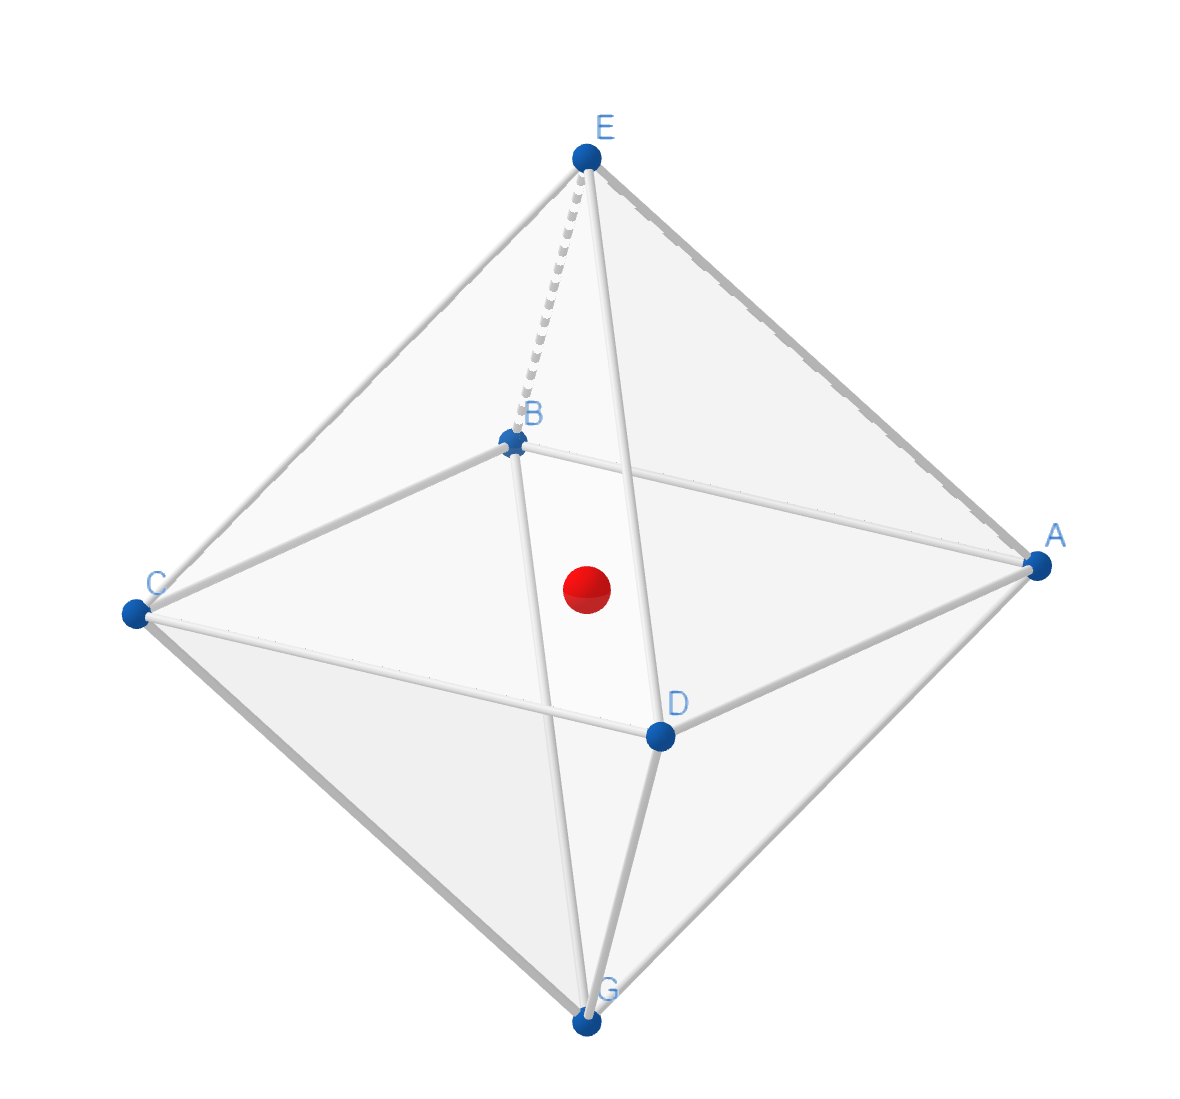
\includegraphics[width=0.8\textwidth]{./pic/p001.png}
\caption{Ti原子在氧八面体的正中心}

\label{dogp01}
\end{figure}
在氢原子的情况下,没有其他的外加条件的情况下,波函数中的主量子数n有着$n^{2}$度简并
,在更复杂的条件下,量子系统中的简并度会受到外加条件的影响而进一步减小。在周期性结构的晶格格点之上,受到周围各向异性排布的其他原子或离子的影响,原子或离子的能级会发生变化。晶体场理论主要是研究在各向异性环境中的原子,根具晶场效应的强弱,可以分为三类。

\paragraph{弱晶场(交换劈裂>自旋轨道耦合>晶场)}
稀土元素是一个典型的例子,稀土元素的4f电子距离原子核比较近,不容易受到其他离子势场的影响,这种情况下弱晶场对系统的影响不大,排在自旋轨道耦合之后。
\paragraph{中晶场(交换劈裂>晶场>自旋轨道耦合)}
过度金属,尤其是3d金属是一个典型的例子,晶场效应大于自旋轨道耦合,洪特定则部分失效,导致轨道磁矩猝灭。
\paragraph{强晶场(晶场>交换劈裂>自旋轨道耦合)}
在这种情况下晶场效应足够强大,以至于洪特定则完全失效,不同层级的波函数可以发生混合,通常发生在4d或5d化合物中间,同时要考虑到中心阳离子的d轨道可能会同外围阴离子的p轨道发生混合,形成部分共价键。这种情况常常是配位场理论的研究范围。

\subsubsection{过渡金属离子的晶体场效应}
对于中等程度的晶体场,过度金属是一个很好的例子。典型的钙钛矿结构的$\text{LaTiO}_{3}$中的$Ti^{3+}$离子。在$\text{LaTiO}_{3}$中$La^{3+}\text{和}O^{2-}$没有未配对电子。系统的磁矩主要是由$Ti^{3+}$的单个未配对电子决定的。这个带有磁矩的未配对电子不仅受到中心阳离子的经典库伦吸引力的影响,而且受到到组成周围氧八面体的六个阴离子的影响,其哈密顿量为:
\begin{equation}
    \mathcal{H}_{3d}(\bm{r})=\mathcal{H}^{\text{(Ti)}}(\bm{r})+\sum^{6}_{\text{j=1}}V^{\text{(O)}}(\bm{r}-\bm{R}_{j})
\end{equation}
除了直接求解薛定谔方程,还可以通过3d轨道的分布规律和氧八面体的几何对称性定性地得到。自由粒子的3d轨道是五重简并的,可以细分为$d_{x^{2}-y^{2}},d_{z^{2}},d_{xy},d_{yz}\text{和}d_{zx}$。在氧八面体内部,前两种d轨道$d_{x^{2}-y^{2}},d_{z^{2}}$的波函数主瓣指向带有负电的氧离子,能级会提高,后三种d轨道$d_{xy},d_{yz}\text{和}d_{zx}$波函数的主瓣方向指向氧八面体中的氧正方形的对角线方向,没有正对着氧离子。能级会下降。五重简并就这样被解除了,分为两组,一组是能量较高的二重态$e_{g}$,和剩下的一组能量降低的三重态$t_{2g}$。与$\text{LaTiO}_{3}$相类似的$La_{2}CuO_{4}$中的$Cu^{2+}$也是由氧八面体包围,也带有一个未成对电子,不同的是对于$Cu^{2+}$d轨道存在9个电子,对应应该考虑空穴的占据状态。

% \begin{figure}[h]
%     \centering
%     \resizebox{\textwidth}{!}{
%     \begin{tikzpicture}[line cap=round,line join=round,>=triangle 45,x=0.4cm,y=0.4cm]
%         \clip(-7.568420055431509,-14.648982459713856) rectangle (30.651216037856322,15.468248877500034);
%         \draw [line width=2pt] (-5,0)-- (5,0);
%         \draw [line width=2pt] (0,5)-- (0,-5);
%         \draw [rotate around={-50.05724853255913:(-0.585,0.685)},line width=2pt,color=uququq,fill=uququq,fill opacity=0.53] (-0.585,0.685) ellipse (0.9009667929793787 and 0.4102330582139209);
%         \draw [rotate around={-129.94275146744084:(0.585,0.685)},line width=2pt,color=uququq,fill=uququq,fill opacity=0.66] (0.585,0.685) ellipse (0.9009667929793787 and 0.4102330582139209);
%         \draw [rotate around={50.05724853255913:(-0.585,-0.685)},line width=2pt,color=uququq,fill=uququq,fill opacity=0.72] (-0.585,-0.685) ellipse (0.9009667929793787 and 0.4102330582139209);
%         \draw [rotate around={129.94275146744087:(0.585,-0.685)},line width=2pt,color=uququq,fill=uququq,fill opacity=0.69] (0.585,-0.685) ellipse (0.9009667929793787 and 0.4102330582139209);
%         \draw (2.114941726218458,4.520121475389473) node[anchor=north west] {$\mathbf{d_{xy},d_{yz},d_{zx}}$};
%         \draw [line width=2pt] (7,0)-- (17,0);
%         \draw [line width=2pt] (12,5)-- (12,-5);
%         \draw [line width=2pt] (19,0)-- (29,0);
%         \draw [line width=2pt] (24,5)-- (24,-5);
%         \draw [rotate around={90:(12,1.1638436934424887)},line width=2pt,fill=black,fill opacity=0.39] (12,1.1638436934424887) ellipse (1.2260171011811196 and 0.38546827317293436);
%         \draw [rotate around={180:(10.83615630655751,0)},line width=2pt,fill=black,fill opacity=0.2] (10.83615630655751,0) ellipse (1.2260171011811196 and 0.38546827317293436);
%         \draw [rotate around={-90:(12,-1.1638436934424887)},line width=2pt,fill=black,fill opacity=0.2] (12,-1.1638436934424887) ellipse (1.2260171011811196 and 0.38546827317293436);
%         \draw [rotate around={0:(13.16384369344249,0)},line width=2pt,fill=black,fill opacity=0.2] (13.16384369344249,0) ellipse (1.2260171011811196 and 0.38546827317293436);
%         \draw [rotate around={0:(24.00254899481813,0)},line width=2pt,fill=black,fill opacity=0.2] (24.00254899481813,0) ellipse (1.6839389847634159 and 0.7648916185947887);
%         \draw [rotate around={90:(24,1.4398026937089552)},line width=2pt,fill=black,fill opacity=0.2] (24,1.4398026937089552) ellipse (1.4398026937087463 and 0.7020750078174347);
%         \draw [rotate around={-90:(24,-1.4398026937089552)},line width=2pt,fill=black,fill opacity=0.2] (24,-1.4398026937089552) ellipse (1.4398026937087463 and 0.7020750078174347);
%         \draw (14.130215120592297,4.520121475389473) node[anchor=north west] {$\mathbf{d_{x^{2}-y^{2}}}$};
%         \draw (26.105964589326746,4.520121475389473) node[anchor=north west] {$\mathbf{d_{z^{2}}}$};
%         \begin{scriptsize}
%         \draw [fill=ududff] (-5,0) circle (2.5pt);
%         \draw [fill=ududff] (5,0) circle (2.5pt);
%         \draw [fill=ududff] (0,5) circle (2.5pt);
%         \draw [fill=ududff] (0,-5) circle (2.5pt);
%         \draw [fill=ududff] (7,0) circle (2.5pt);
%         \draw [fill=ududff] (17,0) circle (2.5pt);
%         \draw [fill=ududff] (12,5) circle (2.5pt);
%         \draw [fill=ududff] (12,-5) circle (2.5pt);
%         \draw [fill=xdxdff] (19,0) circle (2.5pt);
%         \draw [fill=xdxdff] (29,0) circle (2.5pt);
%         \draw [fill=ududff] (24,5) circle (2.5pt);
%         \draw [fill=ududff] (24,-5) circle (2.5pt);
%         \draw [fill=uuuuuu] (12,0) circle (2pt);
%         \end{scriptsize}
%         \end{tikzpicture}
%     }
%     \vspace*{-3cm}
%     \caption{氧八面体中心离子的d轨道\ 简并的5个d轨道由于处于各向异性的势场中,地位不再等同,发生能级分裂,波函数主瓣指向阴离子的轨道能量会上升,波函数主瓣远离阴离子,指向其空隙的能级会下降。}
%     \label{t001}
% \end{figure}


\definecolor{uuuuuu}{rgb}{0.26666666666666666,0.26666666666666666,0.26666666666666666}
\definecolor{xdxdff}{rgb}{0.49019607843137253,0.49019607843137253,1}
\definecolor{uququq}{rgb}{0.25098039215686274,0.25098039215686274,0.25098039215686274}
\definecolor{ududff}{rgb}{0.30196078431372547,0.30196078431372547,1}

\begin{figure}[h]
    \centering
    \resizebox{\textwidth}{!}{
    \vspace*{-3cm}
    \begin{tikzpicture}[line cap=round,line join=round,>=triangle 45,x=0.4cm,y=0.4cm]
        \clip(-7.568420055431509,-14.648982459713856) rectangle (30.651216037856322,15.468248877500034);
        \draw [line width=2pt] (-5,0)-- (5,0);
        \draw [line width=2pt] (0,5)-- (0,-5);
        \draw [rotate around={-50.05724853255913:(-0.585,0.685)},line width=2pt,color=uququq,fill=uququq,fill opacity=0.53] (-0.585,0.685) ellipse (0.9009667929793787 and 0.4102330582139209);
        \draw [rotate around={-129.94275146744084:(0.585,0.685)},line width=2pt,color=uququq,fill=uququq,fill opacity=0.66] (0.585,0.685) ellipse (0.9009667929793787 and 0.4102330582139209);
        \draw [rotate around={50.05724853255913:(-0.585,-0.685)},line width=2pt,color=uququq,fill=uququq,fill opacity=0.72] (-0.585,-0.685) ellipse (0.9009667929793787 and 0.4102330582139209);
        \draw [rotate around={129.94275146744087:(0.585,-0.685)},line width=2pt,color=uququq,fill=uququq,fill opacity=0.69] (0.585,-0.685) ellipse (0.9009667929793787 and 0.4102330582139209);
        \draw (2.114941726218458,4.520121475389473) node[anchor=north west] {$\mathbf{d_{xy},d_{yz},d_{zx}}$};
        \draw [line width=2pt] (7,0)-- (17,0);
        \draw [line width=2pt] (12,5)-- (12,-5);
        \draw [line width=2pt] (19,0)-- (29,0);
        \draw [line width=2pt] (24,5)-- (24,-5);
        \draw [rotate around={90:(12,1.1638436934424887)},line width=2pt,fill=black,fill opacity=0.39] (12,1.1638436934424887) ellipse (1.2260171011811196 and 0.38546827317293436);
        \draw [rotate around={180:(10.83615630655751,0)},line width=2pt,fill=black,fill opacity=0.2] (10.83615630655751,0) ellipse (1.2260171011811196 and 0.38546827317293436);
        \draw [rotate around={-90:(12,-1.1638436934424887)},line width=2pt,fill=black,fill opacity=0.2] (12,-1.1638436934424887) ellipse (1.2260171011811196 and 0.38546827317293436);
        \draw [rotate around={0:(13.16384369344249,0)},line width=2pt,fill=black,fill opacity=0.2] (13.16384369344249,0) ellipse (1.2260171011811196 and 0.38546827317293436);
        \draw [rotate around={0:(24.00254899481813,0)},line width=2pt,fill=black,fill opacity=0.2] (24.00254899481813,0) ellipse (1.6839389847634159 and 0.7648916185947887);
        \draw [rotate around={90:(24,1.4398026937089552)},line width=2pt,fill=black,fill opacity=0.2] (24,1.4398026937089552) ellipse (1.4398026937087463 and 0.7020750078174347);
        \draw [rotate around={-90:(24,-1.4398026937089552)},line width=2pt,fill=black,fill opacity=0.2] (24,-1.4398026937089552) ellipse (1.4398026937087463 and 0.7020750078174347);
        \draw (14.130215120592297,4.520121475389473) node[anchor=north west] {$\mathbf{d_{x^{2}-y^{2}}}$};
        \draw (26.105964589326746,4.520121475389473) node[anchor=north west] {$\mathbf{d_{z^{2}}}$};
        \begin{scriptsize}
        \draw [fill=ududff] (-5,0) circle (2.5pt);
        \draw [fill=ududff] (5,0) circle (2.5pt);
        \draw [fill=ududff] (0,5) circle (2.5pt);
        \draw [fill=ududff] (0,-5) circle (2.5pt);
        \draw [fill=ududff] (7,0) circle (2.5pt);
        \draw [fill=ududff] (17,0) circle (2.5pt);
        \draw [fill=ududff] (12,5) circle (2.5pt);
        \draw [fill=ududff] (12,-5) circle (2.5pt);
        \draw [fill=xdxdff] (19,0) circle (2.5pt);
        \draw [fill=xdxdff] (29,0) circle (2.5pt);
        \draw [fill=ududff] (24,5) circle (2.5pt);
        \draw [fill=ududff] (24,-5) circle (2.5pt);
        \draw [fill=uuuuuu] (12,0) circle (2pt);
        \end{scriptsize}
        \end{tikzpicture}
    }
    \vspace*{-3cm}
    \caption{氧八面体中心离子的d轨道\ 简并的5个d轨道由于处于各向异性的势场中,地位不再等同,发生能级分裂,波函数主瓣指向阴离子的轨道能量会上升,波函数主瓣远离阴离子,指向其空隙的能级会下降。}
    \label{}
\end{figure}

\begin{figure}[h]
    \centering
    \resizebox{\textwidth}{!}{
        \vspace*{-3cm}
        \begin{tikzpicture}[line cap=round,line join=round,>=triangle 45,x=3cm,y=3cm]
            \clip(-4.880291166623681,-2.3485074264249626) rectangle (5.396326222588918,6.000589473883519);
            \draw [->,line width=2pt] (-1,2) -- (1,2);
            \draw [->,line width=2pt] (1,1.5) -- (-1,1.5);
            \draw (-0.31386821851793875,1.4436796223977102) node[anchor=north west] {\parbox{3.167610477296026 cm}{\Huge 温度 \\ 压强 \\ 光照}};
            \draw [line width=2pt] (-2.5,2.5)-- (-2,2.5);
            \draw [line width=2pt] (-3.5,2.5)-- (-3,2.5);
            \draw [line width=2pt] (3.5,2.5)-- (3,2.5);
            \draw [line width=2pt] (2.5,2.5)-- (2,2.5);
            \draw [line width=2pt] (-2.5,1)-- (-3,1);
            \draw [line width=2pt] (-2,1)-- (-1.5,1);
            \draw [line width=2pt] (-3.5,1)-- (-4,1);
            \draw [line width=2pt] (2.5,1)-- (3,1);
            \draw [line width=2pt] (2,1)-- (1.5,1);
            \draw [line width=2pt] (3.5,1)-- (4,1);
            \draw [->,line width=2pt] (-3.9,0.8) -- (-3.9,1.2);
            \draw [->,line width=2pt] (-3.6,1.2) -- (-3.6,0.8);
            \draw [->,line width=2pt] (-2.9,0.8) -- (-2.9,1.2);
            \draw [->,line width=2pt] (-2.6,1.2) -- (-2.6,0.8);
            \draw [->,line width=2pt] (-1.9,0.8) -- (-1.9,1.2);
            \draw [->,line width=2pt] (-1.6,1.2) -- (-1.6,0.8);
            \draw [->,line width=2pt] (1.6,0.8) -- (1.6,1.2);
            \draw [->,line width=2pt] (1.9,1.2) -- (1.9,0.8);
            \draw [->,line width=2pt] (2.7,0.8) -- (2.7,1.2);
            \draw [->,line width=2pt] (3.7,0.8) -- (3.7,1.2);
            \draw [->,line width=2pt] (2.2,2.3) -- (2.2,2.7);
            \draw [->,line width=2pt] (3.2,2.3) -- (3.2,2.7);
            \draw (-3.0680028808603987,0.5637246165935542) node[anchor=north west] {\parbox{5 cm}{\Huge 低自旋态 \\ S=0}};
            \draw (2.4107645957534545,0.5532489617625523) node[anchor=north west] {\parbox{5 cm}{\Huge 高自旋态 \\ S=2}};
            \end{tikzpicture}
    }
    \vspace*{-3cm}
    \caption{在八面体络合物中$Fe^{2+}$能级示意图,在一定条件下两种自旋状态可以相互转化}
    \label{t002}
\end{figure}

\subsubsection{JT效应}
Jahn-Teller定理指出,在对称的非线性分子之中,如果一个体系存在多个简并能级,就会发生自发畸变使得简并消除。仍然以$\text{LaTiO}_{3}$为例子,$Ti^{3+}$处于氧八面体的中心位置,在正常情况下$Ti^{3+}$的五个3d轨道是简并的。在进入氧八面体的形成的各向异性的势场之后,会发生能级分裂,分成两组,三重态$t_{2g}$与二重态$e_{g}$。能量简并情况仍然存在,如果氧八面体沿着z轴方向发生一个拉长$\delta_{z}$,这样z轴方向上的离子距离会变得和xy轴不一样,这样会使得能级发生进一步分裂。

\begin{figure}[h]
    \centering
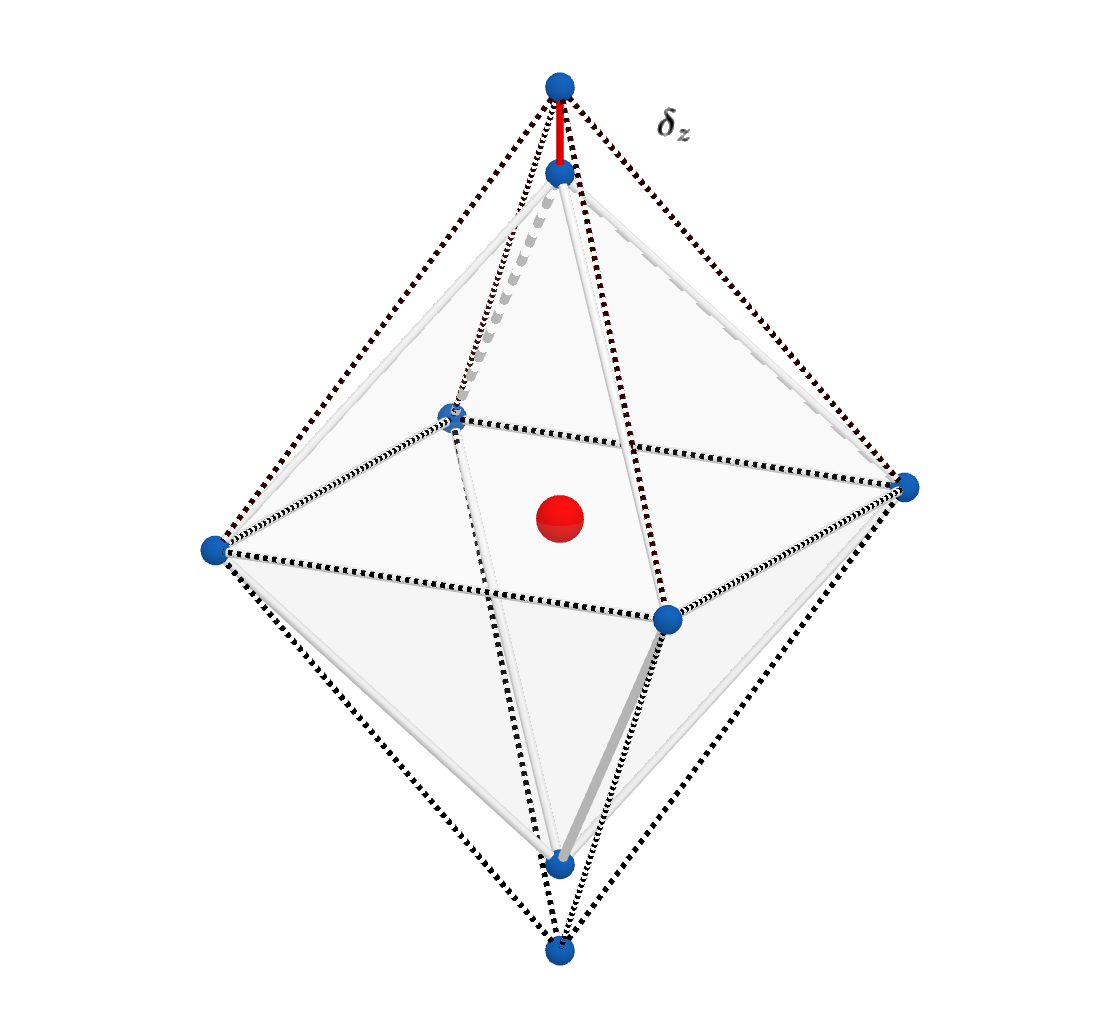
\includegraphics[width=0.8\textwidth]{./pic/p002.png}
\caption{JT效应使得氧八面体发生畸变}

\label{dogp02}
\end{figure}

在$\text{LaTiO}_{3}$发生畸变的情况下,弹性形变使得能量升高$\alpha \delta_{z}^{2}$,电子能级的改变造成的总能量变化与形变值成正比,能量变化为$-\beta \delta_{z}$
。发生形变所造成的整个能量变化为$\alpha \delta_{z}^{2} -\beta \delta_{z}$,这是一个典型的二次函数关系。当能量增量取最小值时$\delta_{z}=\beta /2\alpha $,当整个体系的能量降低时,Jahn-Teller效应就会自发发生。

Jahn-Teller效应最早是在研究分子现象时被发现的,随后推广到晶体之中,在晶体中的Jahn-Teller效应相当复杂。不同的分子或晶格结构会发生不同形式的形变,轨道有序化也伴随着Jahn-Teller配合体有序化,但有些情况下Jahn-Teller效应并不与轨道有序化相耦合,在另一些情况下,Jahn-Teller效应也可能与磁有序相耦合,总之,这是一种相当复杂的效应。

\subsubsection{配位场理论}

在强晶体场的情况下,周围各向异性的离子产生的势能对中心原子或离子的能级影响如此之大以至于可以通过配位的方式形成配位键,这种情况通常出现在过渡金属化合物或配合物,配位基一般是非金属的原子或者分子,常见的主要有$TiF_{6}^{3-}\text{,}Fe(CN)_{6}^{4-}$。通常在处理配位场问题时,需要按照共价键的通用研究方法,考虑共价键、分子轨道等来进行综合考虑。

配位场中的能量分裂也会影响中心离子的磁学性质。以$[Cr(H_{2}O)_{2}]^{2+}$为例,Cr在水分子八面体的各向异性势场当中会发生能级分裂,会分为三重态能量较低的$t_{2g}$和能量比较高的二重态$e_{g}$。Cr有四个价电子,能级较低的$t_{2g}$只能填入三个自旋相同的电子,剩下的那一个电子有两种填充方式,一种时以自旋反平行填充在能级比较低的$t_{2g}$,这种方式所有价电子自旋方向不完全相同,称为低自旋态,另一种是以自旋平行的状态填充到能级较高的$e_{g}$,这种方式所有价电子自旋方向相同,称为高自旋态。具体这两种填充方法在真实情况下如何选择,归根结底还是要整体考虑,看哪一种填充方式总能量更低。通常来讲,周围配位场所造成的能级分裂大小$\Delta$是低自旋态与高自旋态的决定性因素,大的$\Delta$值有利于低自旋态,$\cancel{\Delta}$小则有助于低自旋态的产生。从经验上看来,在d层价电子大于等于八个或者小于等于三个的情况下,有着比较明确的情况,配合物一定会处于高自旋态,但在其他情况下,高自旋态与低自旋态两种情况都有可能出现。在0K的理想条件下,这取决与能量的大小,但在更复杂一些的情况下,多样的外在条件会导致高自旋态与低自旋态之间的转换。例如在八面体中间变得$Fe^{2+}$,其低自旋态的能量稍小于高自旋态的能量,在接近0k的低温下为低自旋态,当温度达到一定程度时,会从低自旋态自发向高自旋态转化,在温度比较高的时候,高自旋态的熵$\Delta S$的影响超过能量的影响,高自旋态的热力学稳定性会提高。


\begin{table}[!htbp]
    \caption{八面体配合物的高自旋态与低自旋态}
    \label{tab:bmt}
    \resizebox{\textwidth}{!}{
    \begin{tabular}{c|c|c|c|c|c|c|c|c}
        \toprule
        \multirow{2}*{$n_{d}$(d电子数)}&\multicolumn{4}{|c|}{高自旋态}&\multicolumn{4}{|c}{低自旋态}\\
        \cline{2-9}
        &$t_{2g}$&$e_{g}$&n&p&$t_{2g}$&$e_{g}$&n&p\\
        \hline
        1&\sout{↑\ }\ \sout{\ \ }\ \sout{\ \ }&\sout{\ \ }\ \sout{\ \ }&1&1.73&&&&\\
        \hline
        2&\sout{↑\ }\ \sout{↑\ }\ \sout{\ \ }&\sout{\ \ }\ \sout{\ \ }&2&2.83&&&&\\
        \hline
        3&\sout{↑\ }\ \sout{↑\ }\ \sout{↑\ }&\sout{\ \ }\ \sout{\ \ }&3&3.87&&&&\\
        \hline
        4&\sout{↑\ }\ \sout{↑\ }\ \sout{↑\ }&\sout{↑\ }\ \sout{\ \ }&4&4.90&\sout{↑↓}\ \sout{↑\ }\ \sout{↑\ }&\sout{\ \ }\ \sout{\ \ }&2&2.83\\
        \hline
        5&\sout{↑\ }\ \sout{↑\ }\ \sout{↑\ }&\sout{↑\ }\ \sout{↑\ }&5&5.92&\sout{↑↓}\ \sout{↑↓}\ \sout{↑\ }&\sout{\ \ }\ \sout{\ \ }&1&1.73\\
        \hline
        6&\sout{↑↓}\ \sout{↑\ }\ \sout{↑\ }&\sout{↑\ }\ \sout{↑\ }&4&4.90&\sout{↑↓}\ \sout{↑↓}\ \sout{↑↓}&\sout{\ \ }\ \sout{\ \ }&0&0\\
        \hline
        7&\sout{↑↓}\ \sout{↑↓}\ \sout{↑\ }&\sout{↑\ }\ \sout{↑\ }&3&3.87&\sout{↑↓}\ \sout{↑↓}\ \sout{↑↓}&\sout{↑\ }\ \sout{\ \ }&1&1.73\\
        \hline
        8&\sout{↑↓}\ \sout{↑↓}\ \sout{↑↓}&\sout{↑\ }\ \sout{↑\ }&2&2.83&&&&\\
        \hline
        9&\sout{↑↓}\ \sout{↑↓}\ \sout{↑↓}&\sout{↑↓}\ \sout{↑\ }&1&1.73&&&&\\
        \bottomrule
    \end{tabular}
    }
\end{table}


\subsection{海森堡模型}

假设在晶体的周期性结构中的格点上面有两个自旋未配对的d电子。根据量子力学以及泡利不相容原理,两个d电子之间的交换能:
\begin{equation}
    E_{ex}=\pm \bm{J}_{12}=\pm \int \phi_{1}^{*}(\bm{r}_{1})\phi_{2}^{*}(\bm{r}_{2})V(\bm{r}_{12})\phi_{1}(\bm{r}_{2})\phi_{2}(\bm{r}_{1})d\bm{r}_{1}d\bm{r}_{2}
    \label{eq:hsb1}
\end{equation}
其中$V(\bm{r})$为系统的库伦相互作用势能,公式中符号对应着自旋的方向。+对应着两个电子自旋方向相反,-号对应两个电子自旋方向相同。

如果考虑到每个离子晶格上未成对的电子大于一个,即每个格点上带有是自旋大于$\frac{1}{2}$,同时忽略同一个离子格点上不同电子之间的交换作用,同时认为量格点上所有电子的交换积分相同,可以得到:
\begin{equation}
    H = -\sum_{l,l'} J_{ll'}\hat{\bm{S}}_{l}\cdot\hat{\bm{S}}_{l'} \ \text{,}\ (l \neq l' )
    \label{eq:hsb2}
\end{equation}
其中$\hat{\bm{S}}_{l}$为在l格点上的自旋算符,$\hat{\bm{S}}_{l‘}$为在l’格点上的自旋算符,$\bm{J}_{ll'}$是格点上电子间的交换积分:
\begin{equation}
    \bm{J}_{ll'}=\bm{J}(|\bm{l}-\bm{l'}|)
    \label{eq:hsb3}
\end{equation}
公式(\ref{eq:hsb2})就是著名的海森堡模型。在实际应用的时候,考虑到交换作用是一种近距离的作用,在长程作用上对整个系统的影响可以忽略不计,在对一般问题的研究中可以只考虑近距离的,尤其是只考虑最近邻的电子交换作用,在各项同性的情况下,海森堡模型可以进一步化简:
\begin{equation}
    H=-J\sum_{l,\delta}\hat{\bm{S}}_{l}\cdot \hat{\bm{S}}_{l+\delta}
    \label{eq:hsb4}
\end{equation}
其中$\delta$为两格点之间的正格矢。当J>0时$\hat{\bm{S}}_{1}\cdot\hat{\bm{S}}_{2}$为正时能量最低,两其个电子自旋方向平行,基态通常为铁磁性。相反的,当J<0时$\hat{\bm{S}}_{1}\cdot\hat{\bm{S}}_{2}$为负时能量最低,两其个电子自旋方向反平行,基态通常为反铁磁性。

海森堡模型的相互作用哈密顿量在时间反演的情况下是不变的,在时间反演操作下,由运动电流产生的磁矩会反向,相互作用哈密顿量会由于两次反向而保持不变,但在外加磁场的情况下,系统的哈密顿量会多出一种外加磁场项$\bm{H}\cdot\bm{S}$这一项会发生改变,外加磁场会破坏系统的时间反演对称性。

\subsection{能带论计算方法}
基于单电子近似能带理论是凝聚态物理的核心问题,多粒子系统中的电子性质的一个有效的解决方法。基于单电子近似的近自由电子理论与紧束缚模型固然可以给出多粒子体系大周期性结构物质之中电子运动的清晰的物理图像,但与实验结果相比偏差过大,难以达到实际使用的要求与应用标准。需要采用更加精确更加可靠的计算方法,如正交平面波方法、赝势法、追加平面波法。这些方法的区别主要在于展开波函数的函数集不同以及用来代替真实晶格之中周期性势能的有效势选取不同。

\subsubsection{正交平面波法}

在周期性结构之中,傅里叶变换是最常用的分析方法之一,傅里叶分解产生的平面波是最简单的正交完备函数集之一。
\begin{equation}
    |\bm{k}+\bm{G}\rangle =\Omega^{-\frac{1}{2}} e^{i(\bm{k}+\bm{G})\cdot\bm{r}}
\end{equation}
晶体之中的波函数可以用平面波展开:
\begin{equation}
    \psi_{\bm{k}(\bm{r})}=\Omega^{-\frac{1}{2}}\sum_{\bm{G}}c(\bm{G})e^{i(\bm{k}+\bm{G})\cdot\bm{r}}
\end{equation}
其中$\Omega$是晶体体积,$\bm{G}$是倒格矢,同样可以对晶体之中的周期性势场进行傅里叶展开,得到傅里叶分解系数:
\begin{equation}
    V(\bm{G}-\bm{G'})=\frac{1}{\Omega}\int d\bm{r}V(\bm{r})e^{-i(\bm{G}-\bm{G'})\cdot\bm{r}}
\end{equation}
将分解后的势场与波函数代入薛定谔方程,即可得到久期方程:
\begin{equation}
    \sum_{\bm{G'}}\{ [\frac{\hbar^{2}}{2m}(\bm{k}+\bm{k})^{2}-E(\bm{k})]\delta_{\bm{G}\bm{G'}}+V(\bm{G}-\bm{G'}) \}c(\bm{G'})=0
\end{equation} 
解这个方程可以得到行列式:
\begin{equation}
    |[\frac{\hbar^{2}}{2m}(\bm{k}+\bm{k})^{2}-E(\bm{k})]\delta_{\bm{G}\bm{G'}}+V(\bm{G}-\bm{G'})|=0
\end{equation}
在使用平面波方法处理这个问题时,没有引入其他的近似条件与简化计算假设,由于平面波函数的正交完备性,原则上可以解决任意周期性势场的问题,只要哈密顿量、势场函数没有问题,理论上完全可以得到正确的结果。然而仅仅使用平面波有一定的局限性。在求解久期方程时,当V(r)为小量时,方程比较好解决。然而在靠近原子核的位置,势场的形式偏离平面波很大,这导致了需要很多项傅里叶系数才可以把势场给展开,同样对于波函数,在离子芯区的波动幅度往往很大,由周期性的平面波展开描述有着天然的缺陷,傅里叶系数的缓慢收敛会导致需要求解的耦合方程数量大大增加。

为了解决平面波方法的缺陷,可以在平面波的基础上加上一个布洛赫函数,使得基函数不仅包括平面波部分,还包括较大动量的孤立原子的波函数,对应的正交平面波为:
\begin{equation}
    \phi_{\bm{k}}(\bm{r})=\Omega^{-\frac{1}{2}}e^{i\bm{k}\cdot\bm{r}}-\sum_{j}\mu_{j\bm{k}}\Phi_{j\bm{k}}(\bm{r})
\end{equation}
其中$\Phi_{j\bm{k}}$时来源于原子轨道$\chi_{j}(\bm{r})$的布洛赫函数:
\begin{equation}
    \Phi_{j\bm{k}}=\frac{1}{\sqrt{N}}\sum_{l}e^{i\bm{k}\cdot\bm{R}_{l}}\chi_{j}(\bm{r}-\bm{R}_{l})
\end{equation}
新的正交化平面波既可以包含远离离子芯区的类似平面波的部分,又包含原子轨道部分。通过波函数的构造方式,波函数与芯态波函数正交。进一步研究可以发现,引入的基于原子轨道的部分相当于在原有的周期性势场的基础上外加了一部分由正交性引起的斥力部分,可以抵消靠近原子核区域的电磁势能的剧烈变化,使得势场的傅里叶变换系数分量减小。

\subsubsection{赝势}
从正交化平面波方法可以导出赝势方法。可以用一个虚假的,比真实的势场要小得多的变化更加平缓的势场$V^{ps}(\bm{r})$代替真实的势场,同时用用一个虚假的波函数$\psi^{ps}$来替代真实的波函数,最终得到一个真实的能量$E(\bm{k})$。真实的波函数:
\begin{equation}
    \psi_{\bm{k}}(\bm{r})=\psi_{\bm{k}}^{ps}-\sum_{j}\mu_{j}\phi_{j}
\end{equation}
其中$\phi_{j}$为原子波函数,将其带入薛定谔方程:
\begin{equation}
    \begin{split}
        &(-\frac{\hbar^{2}}{2m}\nabla^{2}+V)\psi_{\bm{k}}=E(\bm{k})\psi_{\bm{k}} \\
        &(-\frac{\hbar^{2}}{2m}\nabla^{2}+V)\phi_{j}=E(j)\phi_{j}
    \end{split}
\end{equation}
可以得到:
\begin{equation}
    (-\frac{\hbar^{2}}{2m}\nabla^{2}+V^{ps})\psi^{ps}_{\bm{k}}=E(\bm{k})\psi^{ps}_{\bm{k}}
\end{equation}
其中
\begin{equation}
    V^{ps}=V+\sum_{j}(E_{\bm{k}}-E_{j})|\phi_{j}\rangle\langle\phi_{j}|
\end{equation}
赝势的引入使得势场在靠近原子核区域的剧烈变化被抹平,势能在原子核处的奇点也不复存在,波函数靠近原子核的震荡也被消除,成为类似平面波的形式,尽管引入了虚假的势场与波函数,但最终仍然得到了正确的能量。

赝势方法也有其局限性,在过渡元素与稀土元素之中并不是很合适,其根源在于无法明显区分靠近原子核的紧束缚电子和远离原子核的近自由电子。

\subsubsection{缀加平面波}
与近自由电子模型相同,紧束缚模型也可以导出电子的能带结构,将两种不同的思路结合起来,发挥两种途径的优势,避免其缺点是准确计算能带的重要的关键问题。可以采用糕模势来解决这个问题,将势场按照距离原子核的远近分为两个部分,靠近原子核的部分是球对称的原子势,远离原子核的部分是常数势:
\begin{equation}
    V(\bm{r})=
    \begin{cases}
        V_{\alpha}(\bm{r}), & r<r_{c} \\
        0, & r \geq r_{c} \\
    \end{cases}
\end{equation}
其中$r_{c}$是离子芯的半径,也是两种势场的分界半径,$r_{c}$应该小于魏格纳塞斯半径,以保证不同原子的离子芯发生交叠。缀加平面波方法是一种采用糕模势计算能带的常用方法,缀加平面波选取的波函数通常是:
\begin{equation}
    \mathcal{w}_{\bm{k}}=
    \begin{cases}
        \text{原子波函数},  r<r_{c} \\
        \Omega^{-\frac{1}{2}}e^{i\bm{k}\cdot\bm{r}},  r \geq r_{c} \\
    \end{cases}
\end{equation}
在靠近原子核的离子芯区域,缀加平面波采取原子波函数,在外围区域没有势场区域采取平面波,在两者交接处的边界条件,通过选取合适的原子波函数或其线性组合使两个区域的波函数实现平滑连接。得到的$\mathcal{W}_{\bm{k}}$并不能直接拿来用,因为其并不满足布洛赫定理要求的形式,可以通过线性组合的方式构造出符合要求的波函数:
\begin{equation}
    \phi_{\bm{k}}=\sum_{\bm{G}}a(\bm{k}+\bm{G}) \mathcal{W} _{\bm{k}+\bm{G}}
\end{equation}
通过选取合适的系数a,可以实现既满足布洛赫定理的形式,又可以满足边界条件。经过实践的检验,在计算能带方面缀加平面波方法可以以较快的速度得到比较准确的结果。


\begin{figure}[h]
    \centering
    \resizebox{\textwidth}{!}{
    \definecolor{qqqqff}{rgb}{0,0,1}
\definecolor{ududff}{rgb}{0.30196078431372547,0.30196078431372547,1}
\definecolor{zzttqq}{rgb}{0.6,0.2,0}
\definecolor{uuuuuu}{rgb}{0.26666666666666666,0.26666666666666666,0.26666666666666666}
\begin{tikzpicture}[line cap=round,line join=round,>=triangle 45,x=1cm,y=1cm]
\clip(-11.194167526223206,-6.305212530395761) rectangle (16.64612873227008,10.776953581212318);
\fill[line width=2pt,color=zzttqq,fill=zzttqq,fill opacity=0.10000000149011612] (0,0) -- (2,0) -- (3,1.7320508075688774) -- (2,3.4641016151377553) -- (0,3.4641016151377557) -- (-1,1.732050807568879) -- cycle;
\fill[line width=2pt,color=zzttqq,fill=zzttqq,fill opacity=0.10000000149011612] (2,0) -- (0,0) -- (-1,-1.7320508075688774) -- (0,-3.4641016151377553) -- (2,-3.4641016151377557) -- (3,-1.732050807568879) -- cycle;
\fill[line width=2pt,color=zzttqq,fill=zzttqq,fill opacity=0.10000000149011612] (0,0) -- (-1,1.732050807568879) -- (-3,1.7320508075688799) -- (-4,0) -- (-3,-1.7320508075688774) -- (-1,-1.7320508075688792) -- cycle;
\fill[line width=2pt,color=zzttqq,fill=zzttqq,fill opacity=0.10000000149011612] (3,1.7320508075688774) -- (2,0) -- (3,-1.7320508075688772) -- (5,-1.732050807568878) -- (6,0) -- (5,1.7320508075688767) -- cycle;
\fill[line width=2pt,color=zzttqq,fill=zzttqq,fill opacity=0.10000000149011612] (3,1.7320508075688774) -- (5,1.7320508075688767) -- (6,3.464101615137755) -- (5,5.196152422706635) -- (3,5.1961524227066365) -- (2,3.4641016151377584) -- cycle;
\fill[line width=2pt,color=zzttqq,fill=zzttqq,fill opacity=0.10000000149011612] (0,3.4641016151377557) -- (2,3.4641016151377553) -- (3,5.196152422706631) -- (2,6.928203230275508) -- (0,6.92820323027551) -- (-1,5.196152422706634) -- cycle;
\fill[line width=2pt,color=zzttqq,fill=zzttqq,fill opacity=0.10000000149011612] (-3,1.7320508075688799) -- (-1,1.732050807568879) -- (0,3.464101615137758) -- (-1,5.196152422706637) -- (-3,5.196152422706639) -- (-4,3.464101615137761) -- cycle;
\draw [line width=0.8pt,color=qqqqff,fill=qqqqff,fill opacity=0.25] (1.0177639918626207,1.708867528348029) circle (1.2cm);
\draw [line width=0.8pt,color=qqqqff,fill=qqqqff,fill opacity=0.25] (3.9980568028240433,3.4352566566488454) circle (1.2cm);
\draw [line width=0.8pt,color=qqqqff,fill=qqqqff,fill opacity=0.25] (0.999591474722612,5.143473267809653) circle (1.2cm);
\draw [line width=0.8pt,color=qqqqff,fill=qqqqff,fill opacity=0.25] (-2.0356274129362246,3.398539424956995) circle (1.2cm);
\draw [line width=0.8pt,color=qqqqff,fill=qqqqff,fill opacity=0.25] (-2,0) circle (1.2cm);
\draw [line width=0.8pt,color=qqqqff,fill=qqqqff,fill opacity=0.25] (4,0) circle (1.2cm);
\draw [line width=0.8pt,color=qqqqff,fill=qqqqff,fill opacity=0.25] (1.0177639918626207,-1.780255762533621) circle (1.2cm);
\draw [line width=2pt,color=zzttqq] (0,0)-- (2,0);
\draw [line width=2pt,color=zzttqq] (2,0)-- (3,1.7320508075688774);
\draw [line width=2pt,color=zzttqq] (3,1.7320508075688774)-- (2,3.4641016151377553);
\draw [line width=2pt,color=zzttqq] (2,3.4641016151377553)-- (0,3.4641016151377557);
\draw [line width=2pt,color=zzttqq] (0,3.4641016151377557)-- (-1,1.732050807568879);
\draw [line width=2pt,color=zzttqq] (-1,1.732050807568879)-- (0,0);
\draw [line width=2pt,color=zzttqq] (2,0)-- (0,0);
\draw [line width=2pt,color=zzttqq] (0,0)-- (-1,-1.7320508075688774);
\draw [line width=2pt,color=zzttqq] (-1,-1.7320508075688774)-- (0,-3.4641016151377553);
\draw [line width=2pt,color=zzttqq] (0,-3.4641016151377553)-- (2,-3.4641016151377557);
\draw [line width=2pt,color=zzttqq] (2,-3.4641016151377557)-- (3,-1.732050807568879);
\draw [line width=2pt,color=zzttqq] (3,-1.732050807568879)-- (2,0);
\draw [line width=2pt,color=zzttqq] (0,0)-- (-1,1.732050807568879);
\draw [line width=2pt,color=zzttqq] (-1,1.732050807568879)-- (-3,1.7320508075688799);
\draw [line width=2pt,color=zzttqq] (-3,1.7320508075688799)-- (-4,0);
\draw [line width=2pt,color=zzttqq] (-4,0)-- (-3,-1.7320508075688774);
\draw [line width=2pt,color=zzttqq] (-3,-1.7320508075688774)-- (-1,-1.7320508075688792);
\draw [line width=2pt,color=zzttqq] (-1,-1.7320508075688792)-- (0,0);
\draw [line width=2pt,color=zzttqq] (3,1.7320508075688774)-- (2,0);
\draw [line width=2pt,color=zzttqq] (2,0)-- (3,-1.7320508075688772);
\draw [line width=2pt,color=zzttqq] (3,-1.7320508075688772)-- (5,-1.732050807568878);
\draw [line width=2pt,color=zzttqq] (5,-1.732050807568878)-- (6,0);
\draw [line width=2pt,color=zzttqq] (6,0)-- (5,1.7320508075688767);
\draw [line width=2pt,color=zzttqq] (5,1.7320508075688767)-- (3,1.7320508075688774);
\draw [line width=2pt,color=zzttqq] (3,1.7320508075688774)-- (5,1.7320508075688767);
\draw [line width=2pt,color=zzttqq] (5,1.7320508075688767)-- (6,3.464101615137755);
\draw [line width=2pt,color=zzttqq] (6,3.464101615137755)-- (5,5.196152422706635);
\draw [line width=2pt,color=zzttqq] (5,5.196152422706635)-- (3,5.1961524227066365);
\draw [line width=2pt,color=zzttqq] (3,5.1961524227066365)-- (2,3.4641016151377584);
\draw [line width=2pt,color=zzttqq] (2,3.4641016151377584)-- (3,1.7320508075688774);
\draw [line width=2pt,color=zzttqq] (0,3.4641016151377557)-- (2,3.4641016151377553);
\draw [line width=2pt,color=zzttqq] (2,3.4641016151377553)-- (3,5.196152422706631);
\draw [line width=2pt,color=zzttqq] (3,5.196152422706631)-- (2,6.928203230275508);
\draw [line width=2pt,color=zzttqq] (2,6.928203230275508)-- (0,6.92820323027551);
\draw [line width=2pt,color=zzttqq] (0,6.92820323027551)-- (-1,5.196152422706634);
\draw [line width=2pt,color=zzttqq] (-1,5.196152422706634)-- (0,3.4641016151377557);
\draw [line width=2pt,color=zzttqq] (-3,1.7320508075688799)-- (-1,1.732050807568879);
\draw [line width=2pt,color=zzttqq] (-1,1.732050807568879)-- (0,3.464101615137758);
\draw [line width=2pt,color=zzttqq] (0,3.464101615137758)-- (-1,5.196152422706637);
\draw [line width=2pt,color=zzttqq] (-1,5.196152422706637)-- (-3,5.196152422706639);
\draw [line width=2pt,color=zzttqq] (-3,5.196152422706639)-- (-4,3.464101615137761);
\draw [line width=2pt,color=zzttqq] (-4,3.464101615137761)-- (-3,1.7320508075688799);
\begin{scriptsize}
\draw [fill=uuuuuu] (0,0) circle (2pt);
\draw [fill=black] (2,0) circle (2.5pt);
\draw [fill=uuuuuu] (3,1.7320508075688774) circle (2pt);
\draw [fill=uuuuuu] (2,3.4641016151377553) circle (2pt);
\draw [fill=uuuuuu] (0,3.4641016151377557) circle (2pt);
\draw [fill=uuuuuu] (-1,1.732050807568879) circle (2pt);
\draw [fill=uuuuuu] (-1,-1.7320508075688774) circle (2.5pt);
\draw [fill=uuuuuu] (0,-3.4641016151377553) circle (2.5pt);
\draw [fill=uuuuuu] (2,-3.4641016151377557) circle (2.5pt);
\draw [fill=uuuuuu] (3,-1.732050807568879) circle (2.5pt);
\draw [fill=uuuuuu] (-3,1.7320508075688799) circle (2pt);
\draw [fill=uuuuuu] (-4,0) circle (2pt);
\draw [fill=uuuuuu] (-3,-1.7320508075688774) circle (2pt);
\draw [fill=uuuuuu] (-1,-1.7320508075688792) circle (2pt);
\draw [fill=uuuuuu] (3,-1.7320508075688772) circle (2pt);
\draw [fill=uuuuuu] (5,-1.732050807568878) circle (2pt);
\draw [fill=uuuuuu] (6,0) circle (2pt);
\draw [fill=uuuuuu] (5,1.7320508075688767) circle (2pt);
\draw [fill=uuuuuu] (6,3.464101615137755) circle (2pt);
\draw [fill=uuuuuu] (5,5.196152422706635) circle (2pt);
\draw [fill=uuuuuu] (3,5.1961524227066365) circle (2pt);
\draw [fill=uuuuuu] (2,3.4641016151377584) circle (2pt);
\draw [fill=uuuuuu] (3,5.196152422706631) circle (2pt);
\draw [fill=uuuuuu] (2,6.928203230275508) circle (2pt);
\draw [fill=uuuuuu] (0,6.92820323027551) circle (2pt);
\draw [fill=uuuuuu] (-1,5.196152422706634) circle (2pt);
\draw [fill=uuuuuu] (0,3.464101615137758) circle (2pt);
\draw [fill=uuuuuu] (-1,5.196152422706637) circle (2pt);
\draw [fill=uuuuuu] (-3,5.196152422706639) circle (2pt);
\draw [fill=uuuuuu] (-4,3.464101615137761) circle (2pt);
\draw [fill=ududff] (1.0177639918626207,1.708867528348029) circle (2.5pt);
\draw [fill=ududff] (3.9980568028240433,3.4352566566488454) circle (2.5pt);
\draw [fill=ududff] (0.999591474722612,5.143473267809653) circle (2.5pt);
\draw [fill=ududff] (-2.0356274129362246,3.398539424956995) circle (2.5pt);
\draw [fill=ududff] (-2,0) circle (2.5pt);
\draw [fill=ududff] (4,0) circle (2.5pt);
\draw [fill=ududff] (1.0177639918626207,-1.780255762533621) circle (2.5pt);
\end{scriptsize}
\end{tikzpicture}
    }
    \vspace*{-1cm}
    \caption{糕模势示意图\ 选取一个半径r,一刀切地将势场分为两部分,靠近原子核的部分采用原子势,大于半径r的部分直接采用常数势,看起来这是一种十分粗糙的办法,但实践却证明其在其在一定条件下准确有效,其原因是同时兼顾了两种截然不同的势场,抓住主要矛盾与矛盾的主要方面,实现了两点论与重点论的统一}
    \label{}
\end{figure}


\subsection{相对论量子力学}

在不考虑相对论效应的量子力学的情况下,电子自旋并不是非相对论量子力学原生理论的一部分,而是是外加在非相对论量子力学框架之外的一部分,而在相对论量子力学之中,狄拉克方程可以很自然得到电子自旋。随着对材料微观结构的进一步认识和对磁性等自旋电子学研究的深入,相对论量子力学的结论如自旋轨道相互作用对新型材料的电磁性质起着越来越重要的作用。

在相对论量子力学与非相对论量子力学之中,哈密顿量的重要区别之一就是能量动量关系,在相对论中,能量动量的关系:
\begin{equation}
    \label{xdl}
    E^{2}=m_{0}^{2}c^{4}+c^{2}\bm{p}^{2}
\end{equation}
基于相对论导出的动量能量关系,可以改造哈密顿量之中的动能项,根据采用改造方式不同,可能产生不同的相对论量子力学方程。将薛定谔方程对时间导数升为二阶,可以得到描述波色子的克莱因-戈登方程:
\begin{equation}
    (i \hbar \frac{\partial}{\partial t}-q \varPhi )^{2}\varPsi (x,y,z,t)=(-\hbar^{2}c^{2} \nabla^{2} +m^{2}c^{4})\varPsi (x,y,z,t)
    \label{eq:kg}
\end{equation}
其中q为粒子电荷,$\varPhi$为电磁势场。克莱因-戈登无法描述带有自旋的电子的运动,会出现粒子数不守恒的可怕错误。为了解决这个问题,狄拉克提出了另一种相对论微观粒子运动方程,经发现,克莱因-戈登方程无法对电子运动进行描述的根源是对时间的导数改为二阶,通过对相对论能量动量关系进行开方,即可得到狄拉克方程:
\begin{gather}
        (i \hbar \frac{\partial}{\partial t}- c \bm{\alpha} \cdot (-i \hbar \nabla )-\beta m c^{2}) \varPsi =0 \\
        \bm{\alpha} \cdot (-i \hbar \nabla )= \alpha _{x}(-i \hbar \frac{\partial}{\partial x}) +\alpha _{y}(-i \hbar \frac{\partial}{\partial y})+\alpha _{z}(-i \hbar \frac{\partial}{\partial z})
    \label{eq:狄喇克方程}
\end{gather}
其中$\bm{\alpha}$为矢量。为了满足相对论的能量动量关系,公式中的矢量$\bm{\alpha}$和标量$\beta$需要满足一定的关系:
\begin{equation}
    \begin{split}
        &\alpha _{x}^{2}=\alpha _{y}^{2}=\alpha _{z}^{2}=\beta^{2}=1 \\
        &\alpha _{i}\alpha _{j}=\alpha _{j}\alpha _{i}\text{,}j\neq i \\
        &\alpha _{i}\beta+\beta\alpha _{i}=0
    \end{split}
    \label{eq:tj}
\end{equation}
显然,普通的一维数难以满足要求,通过选取合适的矩阵可以满足条件。$\bm{\alpha}\beta$可以用四阶矩阵表示出来。
\begin{equation}
    \bm{\alpha}= \begin{pmatrix}
        0 & \sigma \\
        \sigma & 0
    \end{pmatrix}
    \ , \ \bm{\beta} = 
    \begin{pmatrix}
        \bm{I} & 0\\
        0& \bm{-I}
    \end{pmatrix}
    \label{eq:pl1}
\end{equation}
其中$\bm{I}$是单位矩阵,$\bm{\sigma}$是泡利矩阵:
\begin{equation}
    \sigma _{1} =
    \begin{pmatrix}
        0 & 1 \\
        1 & 0
    \end{pmatrix}
    \ , \ 
    \sigma _{2} = 
    \begin{pmatrix}
        0 & -i \\
        i & 0
    \end{pmatrix}
    \ , \ 
    \sigma _{2} = 
    \begin{pmatrix}
        1 & 0 \\
        0 & -1
    \end{pmatrix}
    \label{eq:pl2}
\end{equation}
应用狄拉克方程对自由电子进行求解,最终得到的波函数是四分量的波函数,包含着两种自旋方向与正反粒子。其中两个是正能态,另外两个是负能态。狄拉克对负能态的解释是负能态已经被电子充满,形成了电子海,正能态的电子由于泡利不相容不能跃迁到能级更低负能级之上。如果负能海缺失了一个电子,就会出现一个带有正电的空穴,从另一个角度上看来,就会多出一个正电子。电子-空穴理论是现代半导体理论的基础之一。在狄拉克的相对论量子力学的基础上向更高能级、更小尺度上发展出基于量子场论的量子电动力学,可以对电子正电子进行更全面的描述。如果要获得更加精确的数值解,量子电动力学的相关结论不可忽略,量子电动力学对凝聚态物理产生的影响主要有三个,一个是真空涨落,真空不空,时时刻刻存在着涨落现象,会对靠近原子核的电子库伦静电势产生影响。二是真空极化,真空中可能会自发出现正负电子对,使靠近原子核的一定空间范围内对电子的吸引力增加。另一个是延迟效应,在两原子系统中,能量以电磁辐射的形式传递时受制于电磁波的有限传播速度会产生延迟,使得$R^{-6}$的色散力变为$R^{-7}$。





\section{密度泛函理论}

量子力学的密度泛函理论(DFT)核心思想是以粒子密度分布函数代替波函数,作为系统变量,通过求解薛定谔方程,构建能量泛函,最终导出系统的各种物理性质。由量子力学基本原理可以得知,微观系统状态可以采用波函数来描述。写出系统的哈密顿量,通过求解薛定谔方程,解得系统的波函数,原则上就可以得到系统所有的微观信息。但是,在多体问题与多自由度问题上,直接解出薛定谔方程十分困难。然而只要采取合理的近似,可以绕过对波函数的求解,不通过波函数得到相应的物理信息。
\begin{figure}[h]
    \centering
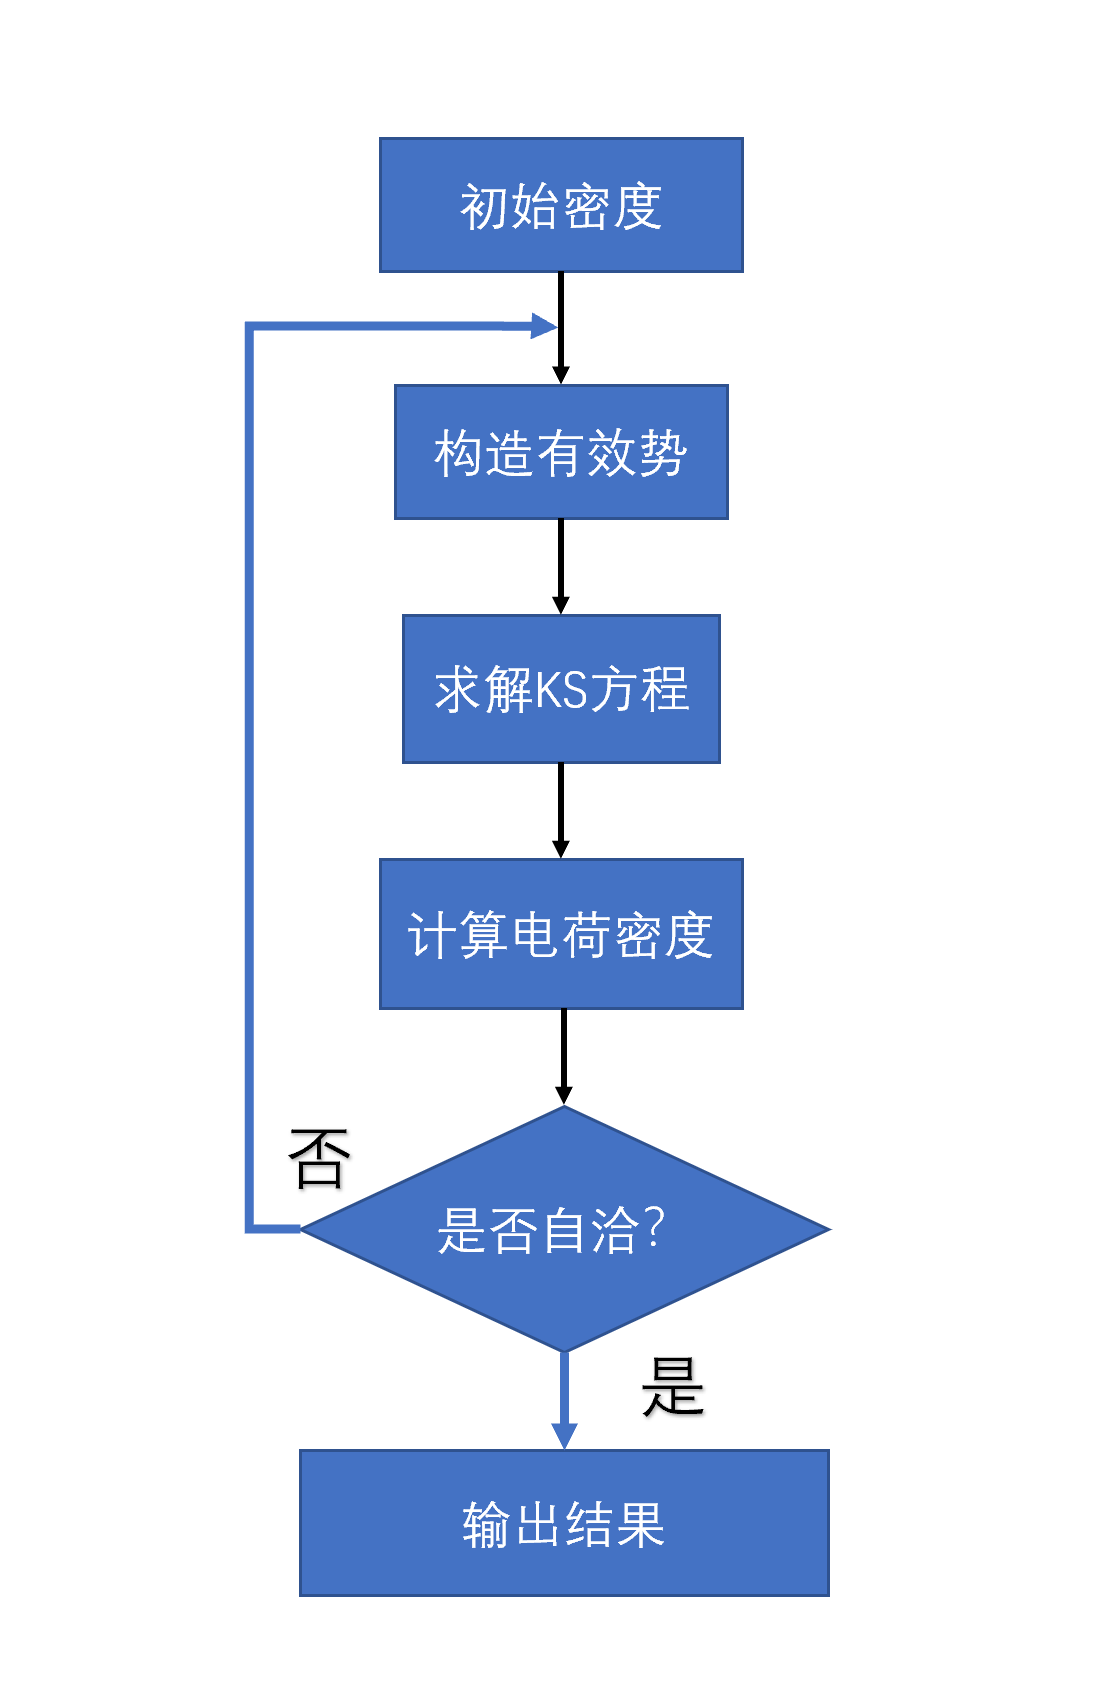
\includegraphics[width=0.5\textwidth]{./pic/012.png}
\caption{自洽求解KS方程流程图}

\label{dog012}
\end{figure}

霍恩伯格和科恩证明了两个重要的定理,即霍恩伯格-科恩第一定理与霍恩伯格-科恩第二定理,是密度泛函理论的基础。

\paragraph{霍恩伯格-科恩第一定理}
对于一个多粒子系统,外场$V(r)$是粒子密度分布函数$\rho(r)$的唯一泛函。由于外场确定后整个系统的哈密顿量就确定了,因此多粒子系统的基态也是密度分布函数的唯一泛函。

\paragraph{霍恩伯格-科恩第二定理}
如果是真实正确的电子密度分布函数,所得到的能量一定是最小值,即是所谓的变分原理。在实际使用时,如果采用近似的哈密顿量,得到的结果有可能会小于基态能量。

基于以上几个理论,可以得出与之对应的霍恩伯格-科恩泛函。
$$F_{HF}[\rho]=\min_{\Phi \to \rho} \langle {\Phi} |\hat{T}+\hat{U}_{ee}|\Phi \rangle =T[\rho]+U_{ee}[\rho]   $$

其中$T[\rho]$和$U_{ee}[\rho]$分别为电子动能泛函与库伦势能泛函。体系的总能量泛函可以写成:
$$E[\rho]=F_{HF}[\rho]+\int \rho(r)V(r)dr=T[\rho]+U_{ee}[\rho]+V[\rho]$$
由粒子总数为定值这一限定条件,求解体系能量最小值,可以应用拉格朗日乘数法等方式找到最低能量和与最低能量相一致的密度分布。在约束条件粒子总数为N,可以导出:
$$\delta\{T[\rho]+U_{ee}[\rho]+V[\rho] - \mu[\int \rho(r)V(r)dr-N]   \} =0$$
直接写出上面各项是十分困难的,需要进一步的近似处理。\cite{becke1992density}
对电子间相互作用这一项,可以写成两部分,一部分与库伦势能平方反比有关,另一部分是交换关联泛函,电子间的交换相关来源于费米子的反对称特性,是所有计算之中最复杂的一部分。
$$ U_{ee} = \frac{1}{2} \iint \frac{\rho (r) \rho (r') }{|r-r'|} drdr'+E_{XC}$$

Kohn和Sham提出过一个利用辅助的等价的无相互作用粒子系统的动能($T_{R}[\rho]$)替代由相互作用的系统的动能($T[\rho]$)。
$$F[\rho]=T_{R}[\rho]+\frac{1}{2} \iint \frac{\rho (r) \rho (r') }{|r-r'|} drdr'+E_{XC}$$
由薛定谔方程及动能算符可得
$$T_{R}[\rho]=\sum_{n = 1}^{N}\langle \Phi_{i} | -\frac{1}{2} \nabla^{2}| \Phi_{i} \rangle   $$
系统的能量泛函可以写成
$$E_{KS}[\rho]=\int \rho(r)V(r)dr+T_{R}[\rho]+\frac{1}{2} \iint \frac{\rho (r) \rho (r') }{|r-r'|} drdr'+E_{XC}$$
对总能量泛函做变分,最终可以得到著名的自洽KS方程\cite{kohn1965self}:
$$[-\frac{1}{2} \nabla^{2}+V_{eff}^{(i)}]\varphi_{i,s}(r)= \varepsilon _{i,s}\varphi_{i,s}(r)$$
$$V_{eff}=V(r)+\iint \frac{ \rho (r') }{|r-r'|} drdr'+\frac{\delta E_{XC}[\rho]}{\delta \rho[r]}$$
$$\rho(r)=\sum_{i = 1}^{N} \sum_{s = 1}^{2}|\varphi_{i,s}(r)|^{2}   $$
当交换关联能泛函形式确定之后,即可通过迭代方法求解KS方程。

对交换关联能的近似需要在满足关联函数对称性和求和规则,常用是近似方法有局域密度近似、广义梯度近似、meta-GGA泛函、杂化泛函等。
\paragraph{局域密度近似}局域密度近似(LDA)基本思想是将非均匀电子气看作是有无穷小体积元内部局域均匀电子气组成,利用均匀电子气的交换关联来近似非均匀电子气。经过近似之后可以得到交换关联泛函:
$$E_{XC}^{LDA}[\rho_{\uparrow}(r),\rho_{\downarrow}(r)]=\int [\rho_{\uparrow }(r)+\rho_{\downarrow}(r)]\varepsilon _{XC}^{h}[\rho_{\uparrow}(r),\rho_{\downarrow}(r)]dr$$
其中$\rho_{\uparrow}(r),\rho_{\downarrow}(r)$分别代表上自旋与下自旋的电子密度,$\varepsilon _{XC}$为均匀电子气的交换关联能密度。局域密度近似更适用于均匀密度体系,在非均匀密度体系,如原子体系,金属表面等与实际情况差异较大。\cite{黄美纯2000密度泛函理论的若干进展}
\paragraph{广义梯度近似} 广义梯度近似(GAA),是将交换关联能按照电子密度及其梯度展开:

$$E_{XC}[\rho]=\int \rho(r) \varepsilon _{XC} [\rho (r)]dr+\int F_{XC}[\rho (r) , \nabla   \rho(r)]dr $$

其中$\varepsilon_{XC}$为电子关联能密度,$F_{XC}$是与某些交换关联空穴性质有关的泛函。
\paragraph{meta-GGA泛函} meta-GGA泛函通过引入轨道动能密度,对广义梯度近似进行修正和改进。
$$E_{XC}^{meta-GGA}[\rho(r)]=\int \rho(r)\varepsilon_{XC}[\rho(r),\nabla \rho(r),\nabla^{2} \rho(r),\tau]dr$$
$$\tau(r)=\sum_{i} |\nabla\Phi_{i} | ^{2}$$
\paragraph{杂化泛函} 通过对GGA与HF形式的交换能按照一定比例混合起来,得到杂化泛函。类似的,可以同时把多种近似形式混合起来。不同的混合方式与混合比例所得到的杂化泛函有着不同的特点与作用形式。

求解KS方程固然可以使用变分法,但是最常用的是自洽场方法。\cite{黄时中1998双电子体系的简单自洽场计算} 自洽场方法首先猜测一个初始的电荷密度,通过这个电荷密度构造出有效势与哈密顿量。通过这个哈密顿量可以解得波函数与能量本征值。所得的波函数又可以重新构造一个电荷密度。利用新得到的电荷密度代替原来的电荷密度,然后反复迭代循环。如果前后两次得到的电荷密度相差达到所设定的精度差,即可认为电荷密度已经收敛。

\section{对称性与空间群}

在凝聚态物理的研究中,对称性有着极其重要的地位,物质的各种存在形式都有着或多或少的对称性,对物质性质变化其决定性作用的相变也与对称性的产生与消失有着密切的联系。在多铁二维材料的研究中,铁磁性与铁电性的出现基本上都是与一种或多种的对称性破缺有关,在高对称结构中寻找对称性的破缺是寻找铁电铁磁材料的关键点之一。

\subsection{对称性极其操作}

对于某些物理量$\rho(r)$,以与空间位置r有关,可以引入一个坐标变换的操作g,使得坐标按照一定的规则发生变化:
\begin{equation}
    \bm{r} \rightarrow  g\bm{r} = \bm{r}'
\end{equation}
坐标的变化同样会使得依赖于坐标的物理量发生变化,如果这个物理量在变化前后依然相等,那么这个物理量在变换操作g下具有对称性。
\begin{equation}
    \rho (\bm{r}') = \rho (g \bm{r}) = \rho (\bm{r})
\end{equation}

在三维空间中,可以简单地采用直角坐标系来表示一个点的位置,而对坐标的变化操作可以分解为两部分,平移部分与非平移部分。平移部分可以用位矢的直接相加减来描述,非平移部分可以采用矩阵乘法来描述:
\begin{gather}
    \bm{r}(x,y,z) \rightarrow \bm{r}'(x',y',z') \\
    \bm{r}'=g\bm{r}=\bm{M}\bm{r}+\bm{t} \\
    \bm{M}=(a_{ij})= \begin{pmatrix}
        a_{11}&a_{12}&a_{13}\\
        a_{21}&a_{22}&a_{23}\\
        a_{31}&a_{32}&a_{33}
    \end{pmatrix}
    \\
    x_{i}' = \sum_{j} a_{ij} x_{j}+t_{i}
\end{gather}
对于狭义的对称性来说,对象内部任意两点的直线距离不会发生变化,这意味着在狭义对称操作下,被操作对象不会发生膨胀与压缩现象。

对与点对称,变换矩阵的行列式应该满足矩阵的行列式的绝对值为1,即:
\begin{equation}
    |\bm{M}|=|a_{ij}|=\pm 1
\end{equation}
以绕Z轴从α转动到β为例:
\begin{equation}
    \bm{M}_{1} = 
    \begin{pmatrix}
        cos(\beta - \alpha) & -sin(\beta - \alpha) & 0\\
        sin(\beta - \alpha) & cos(\beta - \alpha) & 0\\
        0 & 0 & 1 
    \end{pmatrix}
\end{equation}
对与以XY平面为对称面的面对称操作:
\begin{equation}
    \bm{M}_{2} = \begin{pmatrix}
        1 & 0&0\\
        0&1&0\\
        0&0&-1
    \end{pmatrix}
\end{equation}
对坐标原点的中心反演对称操作:
\begin{equation}
    \bm{M}_{3} = \begin{pmatrix}
        -1 & 0&0\\
        0&-1&0\\
        0&0&-1
    \end{pmatrix}
\end{equation}
通过观察计算$M_{1}M_{2}M_{3}$可以发现,$|M_{1}|=+1$而$M_{2}M_{3}$的绝对值为-1。通过对变化矩阵行列式的计算,可以将变化g分为两类$g^{\uppercase\expandafter{\romannumeral1}}g^{\uppercase\expandafter{\romannumeral2}}$,一种变换矩阵的行列式为正,另一种变换矩阵的行列式为负。对与多次连续变换,依据矩阵乘法与行列式规则可以得到,第一类变换的组合或连续变换的结果仍然为第一类变换,第二类变换的偶数次连续变换为第一类变换,奇数次变换为第二类变换:
\begin{equation}
    |\bm{M}(g)|= | \bm{M}(g_{1}^{\uppercase\expandafter{\romannumeral2}}  g_{2}^{\uppercase\expandafter{\romannumeral2}} g_{3}^{\text{\uppercase\expandafter{\romannumeral2}}} \cdots g_{q}^{\uppercase\expandafter{\romannumeral2}})|=(-1)^{q}= \begin{cases}
        +1, &\text{q为偶数}\\
        -1, &\text{q为奇数}
    \end{cases}
\end{equation}

除了行列式上的不同之外,这两类变换还有着更明显更加显著的区别,第一种变换可以通过物体在空间位置上的运动来实现,而第二种对称变换操作则不能在实空间内通过位置的改变实现,必须同过别的方式变换,以手性分子为例,左旋分子是无法在不改变化学键的基础上仅仅通过空间运动来转化成为右旋分子的。

\begin{figure}[]
    \centering
    \resizebox{\textwidth}{!}{
        \subfigure[]{
            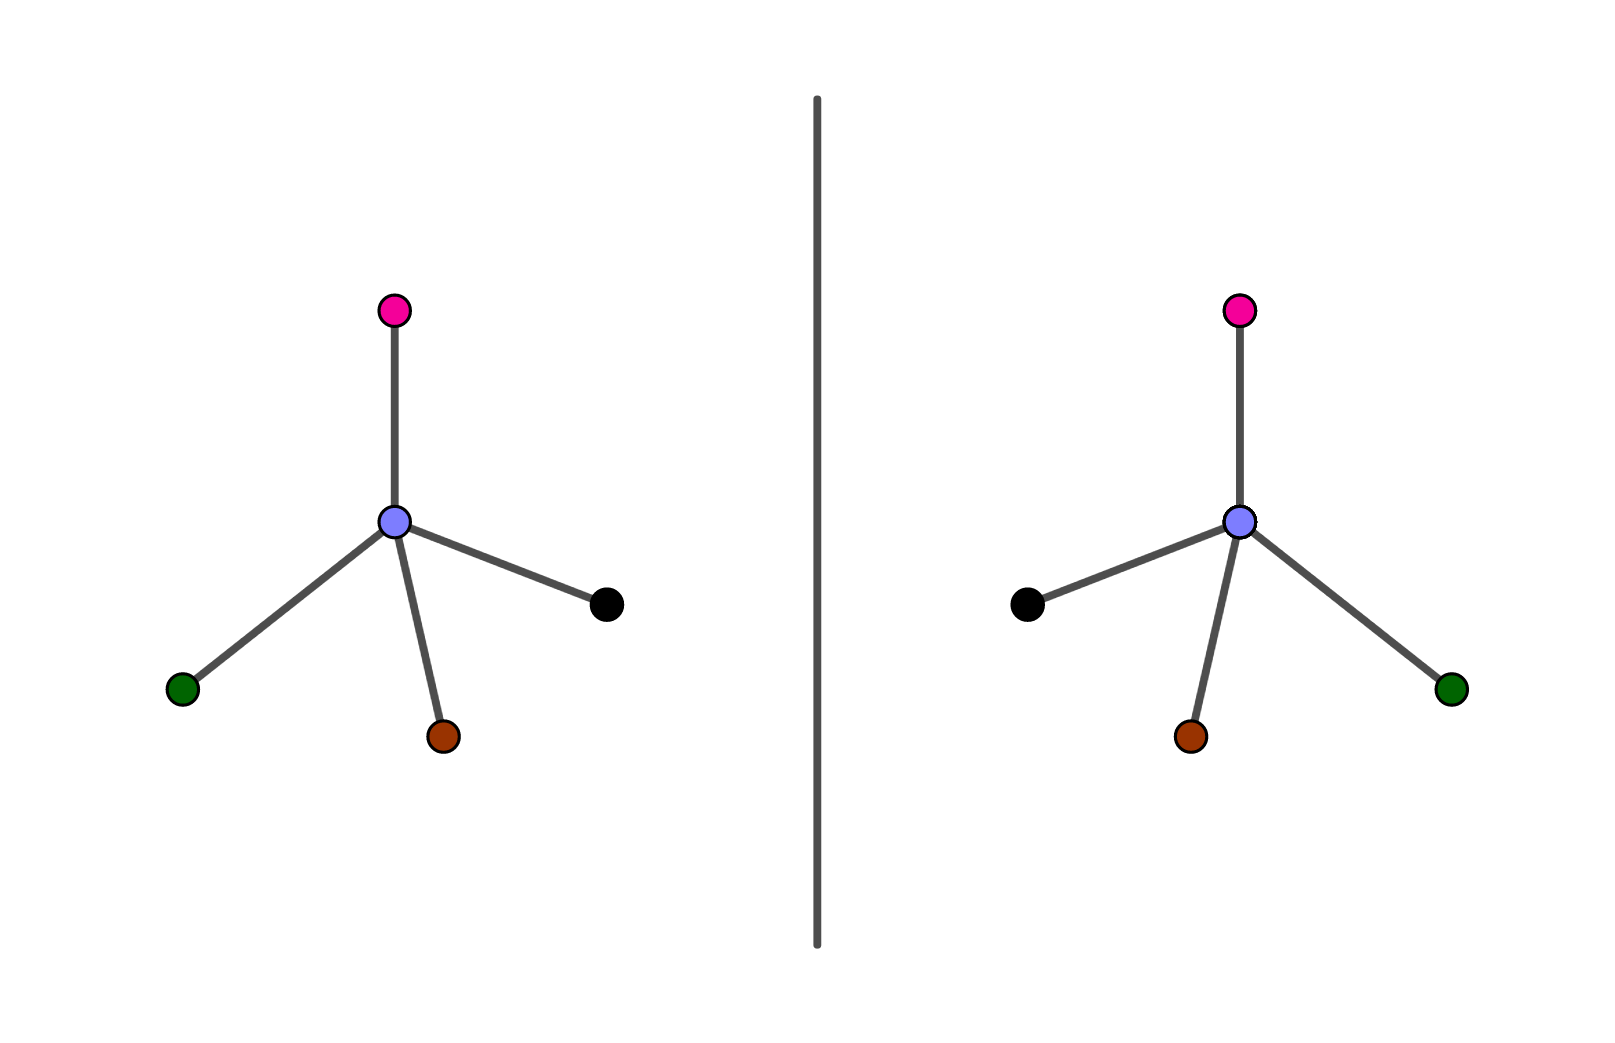
\includegraphics[]{pic/p007.png}
        }
        \subfigure[]{
            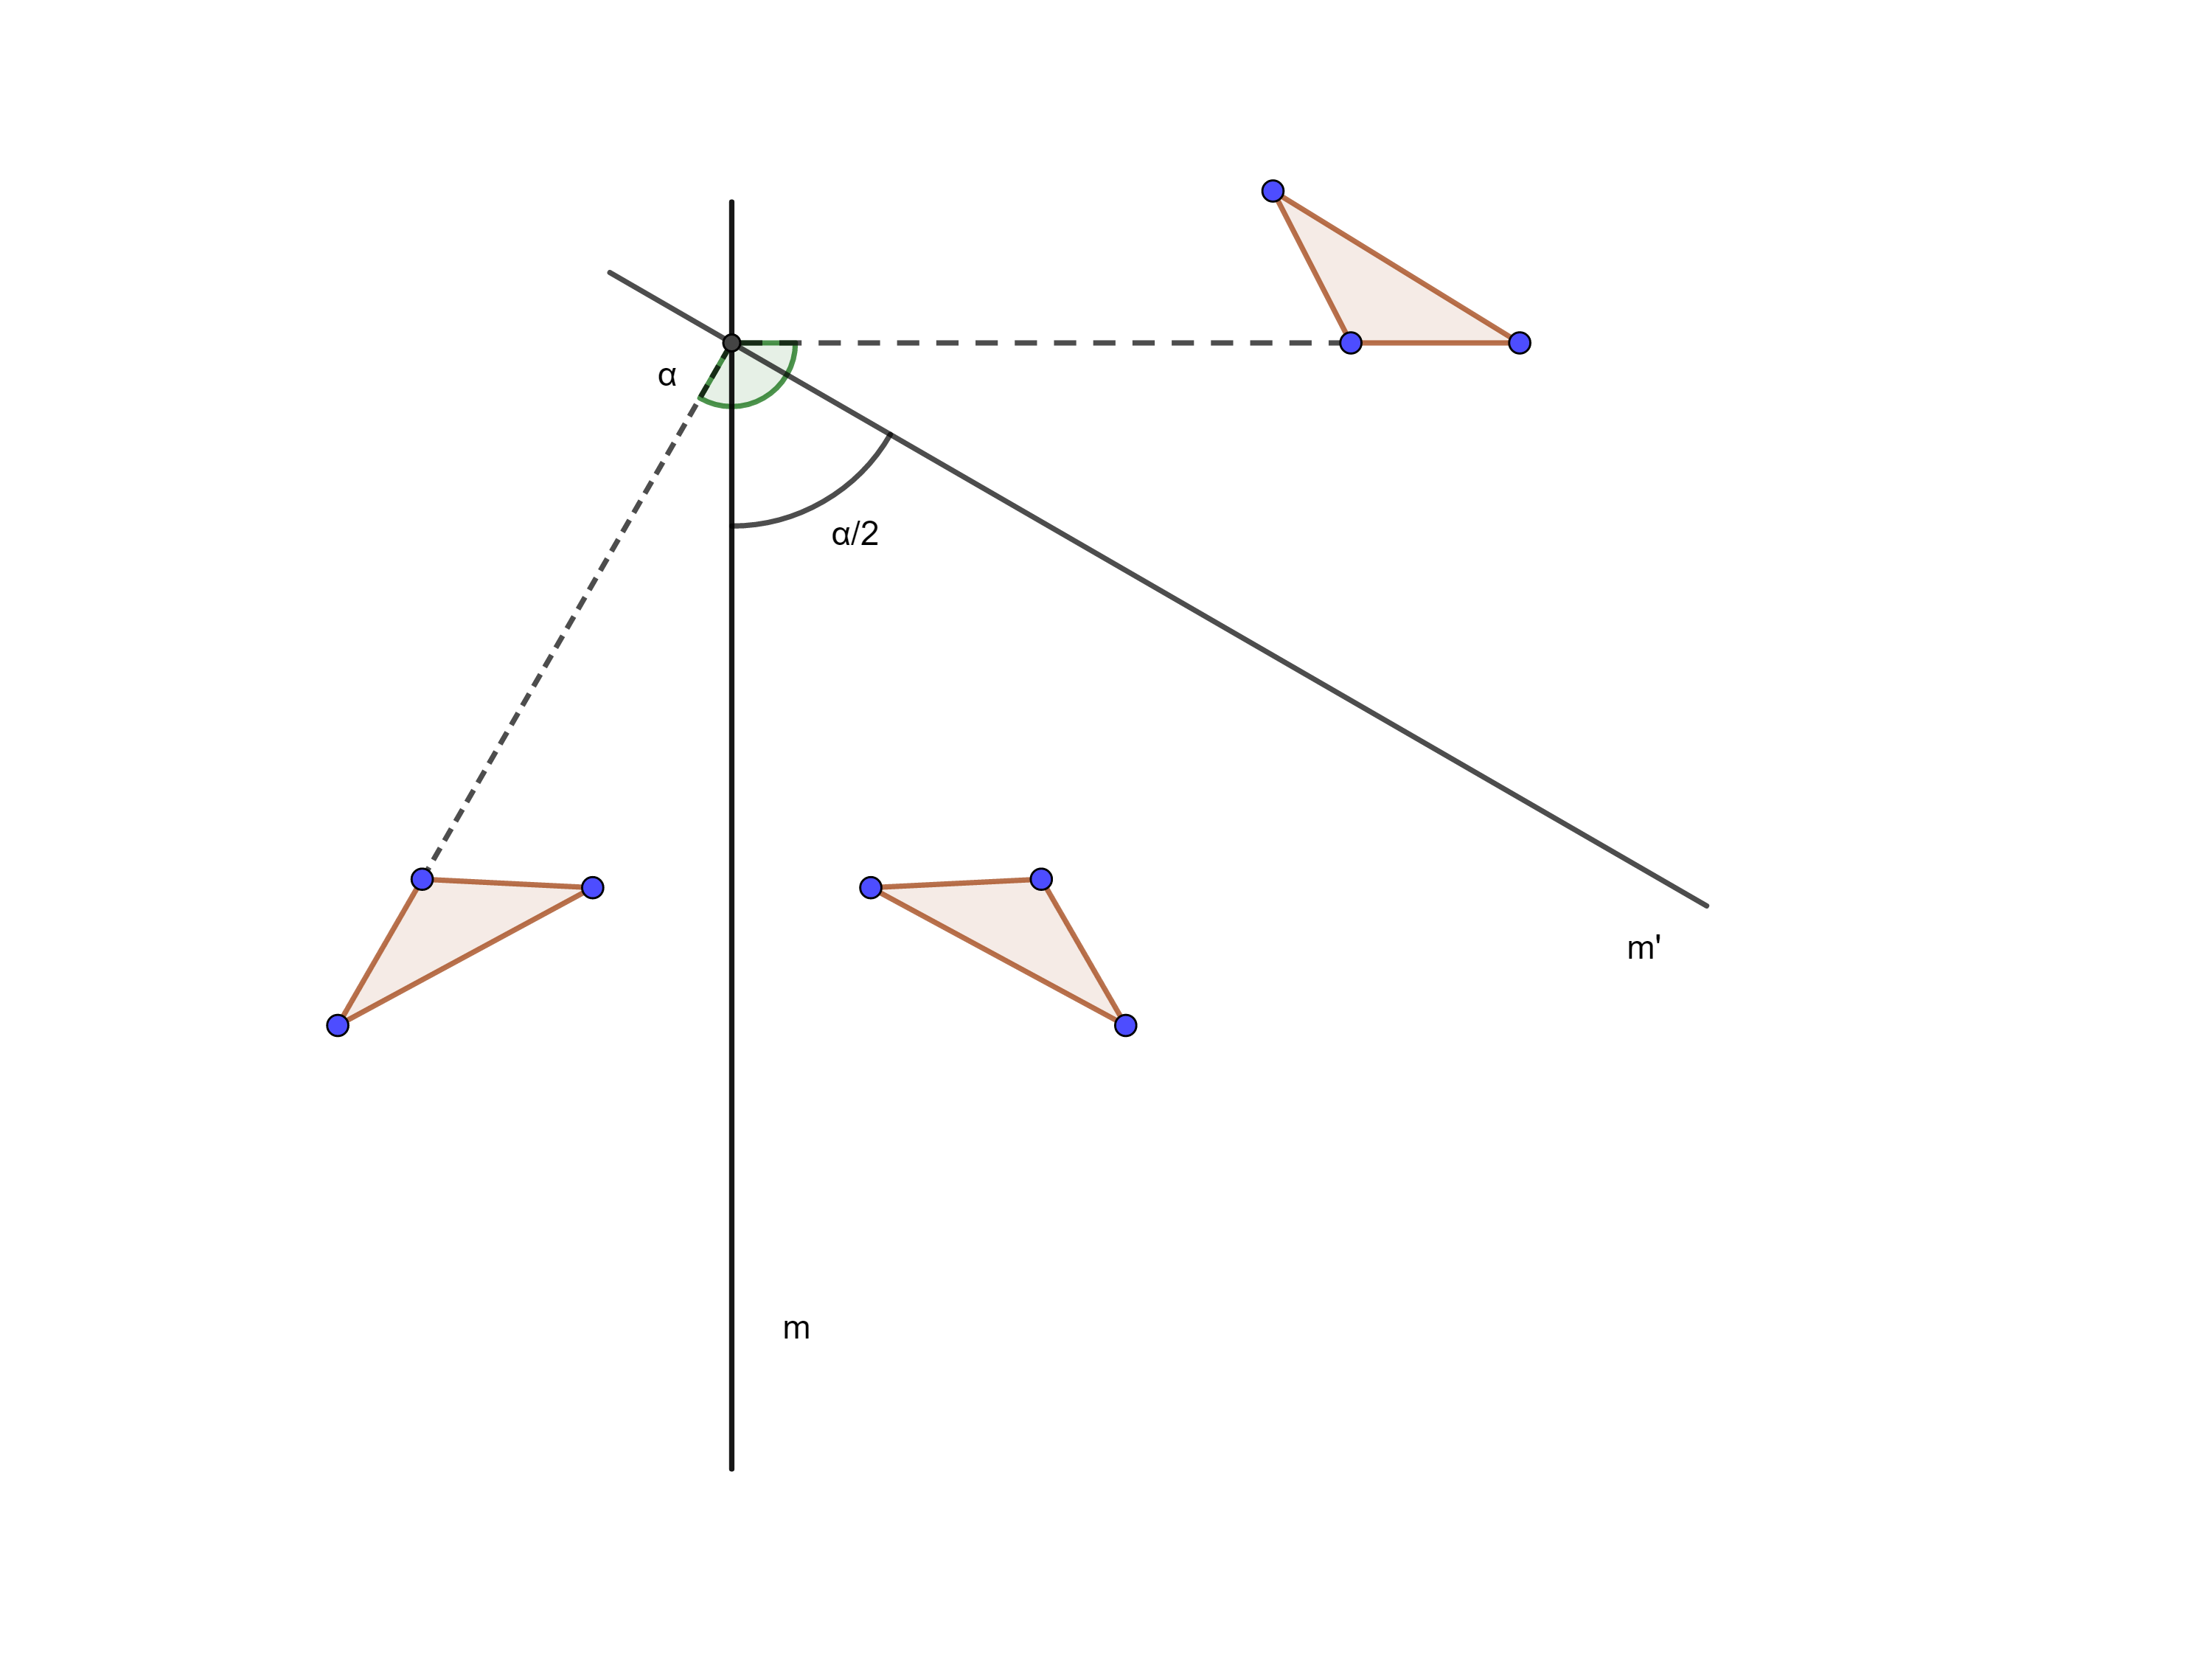
\includegraphics[]{pic/p006.png}
        }
    }
    \caption{(a)手性分子的对称性,左旋分子无法通过空间位置操作转化为右旋分子。(b)万花筒定理}
    \label{p006p007}
\end{figure}

\subsection{对称元素的组合定理}

\paragraph{镜面旋转与反演旋转等价}
镜面旋转$\tilde{N}_{\alpha} $与反演旋转$\bar{N}_{\beta}$等价,即$\tilde{N}_{\alpha} =  \bar{N}_{\pi - \alpha}$。

\paragraph{万花筒定理}
当两个夹角为$\alpha/2$的镜面m与m'的交线相当于转轴$N_{\alpha}$,这个定理是用来制作万花筒的理论依据。

\paragraph{Euler定理}
绕两条相交转轴$N_{\alpha 1}\text{和}N_{\alpha 2}$的先后两次旋转相当于绕第三条轴$N_{\alpha 3}$的旋转,即:
\begin{equation}
    N_{\alpha 1} +N_{\alpha 2}=N_{\alpha 3}
\end{equation}

这三条定理大大减少了对称性元素的组合复杂度,使得对称性理论变得简单。

\subsection{对称群}

对称性与对称性的组合问题需要用群论这个数学工具才能更好地研究明白,一个确定物体的所有对称性操作构成一个对称群的一组元素。群是群论的核心内容,群的概念由群的四个公理定义出来:

\paragraph{封闭性}
群元素的乘积也是一个群元素,以对称群为例,对称群中的两个元素的乘积,也就是两种对称性操作的连续操作等效与群中的另外一个元素(操作),即:$g_{i} \in G , g_{j} \in G  \rightarrow g_{i}g_{j} =g_{l} \in G $。

\paragraph{结合律}
群元素的乘积满足结合律,即:$g_{i}(g_{j}g_{l})=(g_{i}g_{j})g_{l}$。

\paragraph{存在恒等元素}
存在恒等元素e,使得$\text{对于任何}g_{i} \in G \text{,都有} eg_{i}=g_{i}$。

\paragraph{存在逆元素}
对于G中任一元素$g_{i}\text{都有一个逆元素}g^{-1}_{i}\text{使得}g_{i}g_{i}^{-1}=e$。

在通常的群中,一般不存在交换律或交换律不成立,即$g_{i}g_{j} \neq g_{j}g_{i}$,群元素交换次序之后和原来不同,但在特殊的阿贝尔群中,两个元素交换不变$g_{i}g_{j} = g_{j}g_{i}$。不同的群有着不同数目的元素,一个群中包含的元素数目叫群的阶。在一个群内部,如果挑选出部分元素,仍然符合群的定义,可以组成一个规模比较小的子群,子群的阶数一般会小于原来群的阶数。

\subsection{二维平面周期性结构}

周期性原子排列不仅仅是普通的三维材料的研究重点,在二维材料中也是一个十分重要的方面。在三维空间中有着十四种布喇菲格子,但在二维空间中由于对称性比三维空间中要更简单,二维空间中仅有五种布喇菲格子,分别为:斜方、长方、菱形、正方和六角。


\begin{figure}[htbp]
    \centering
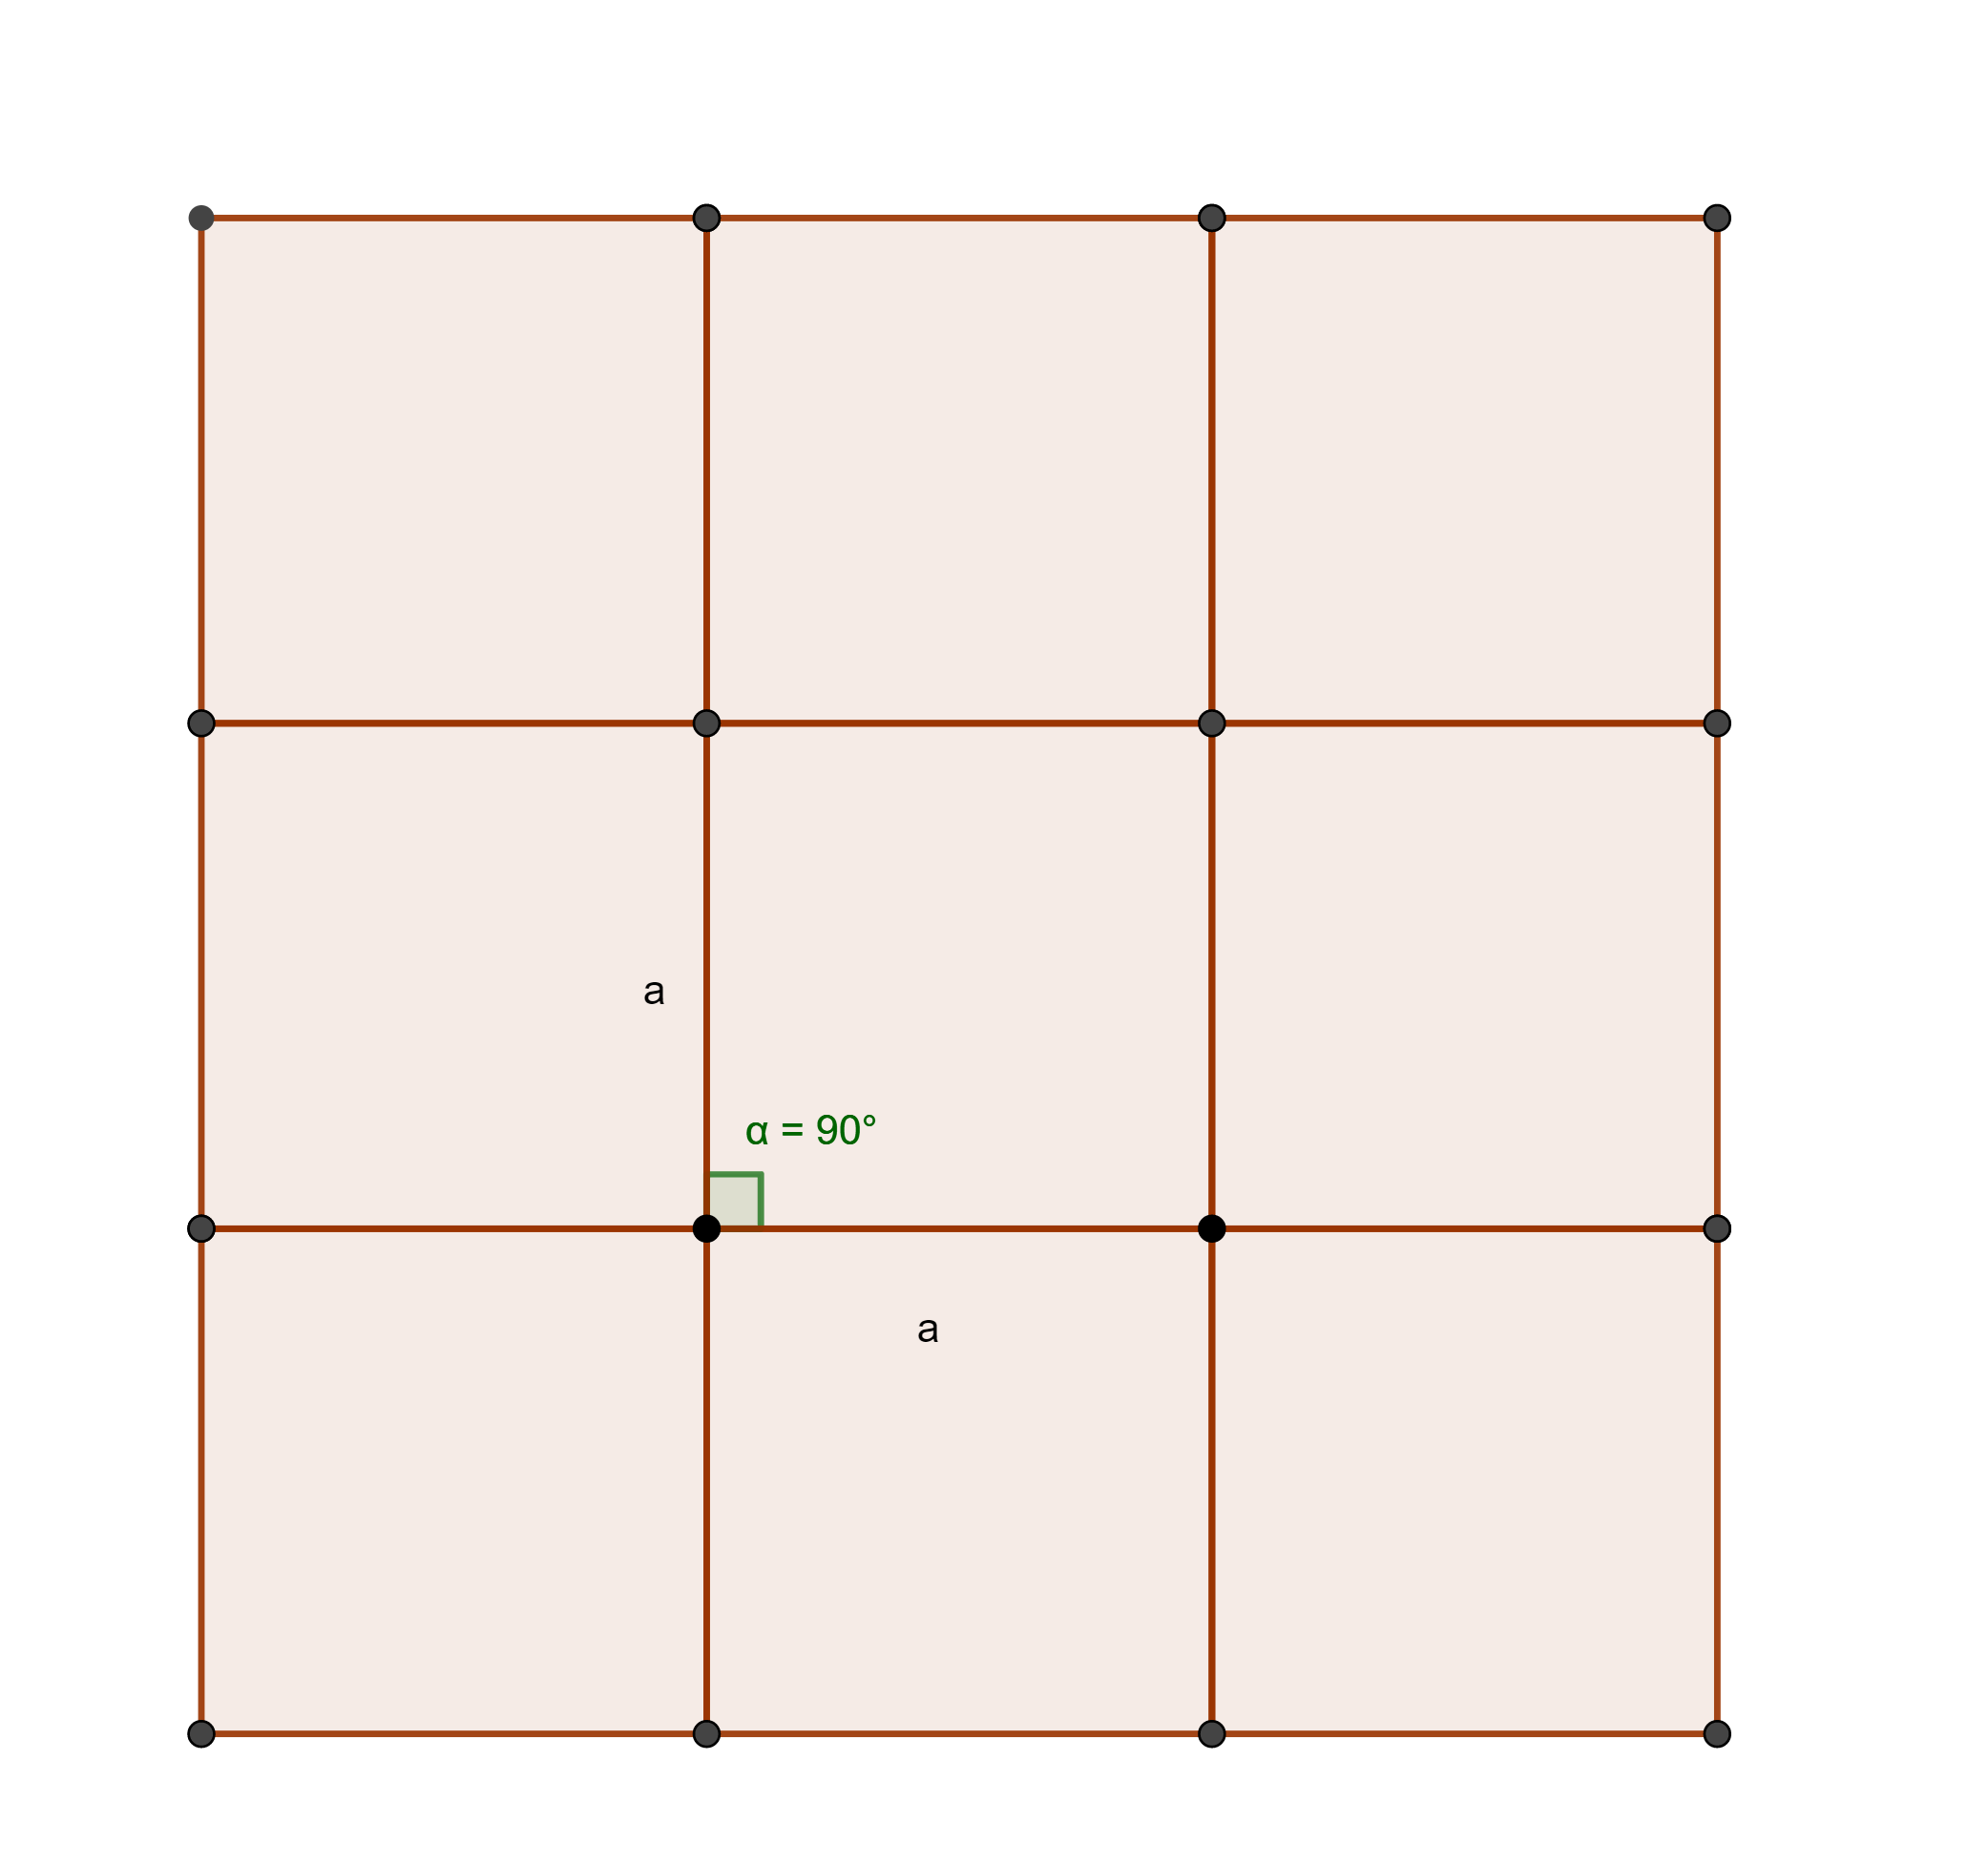
\includegraphics[width=0.4\textwidth]{./pic/p008-1.png}
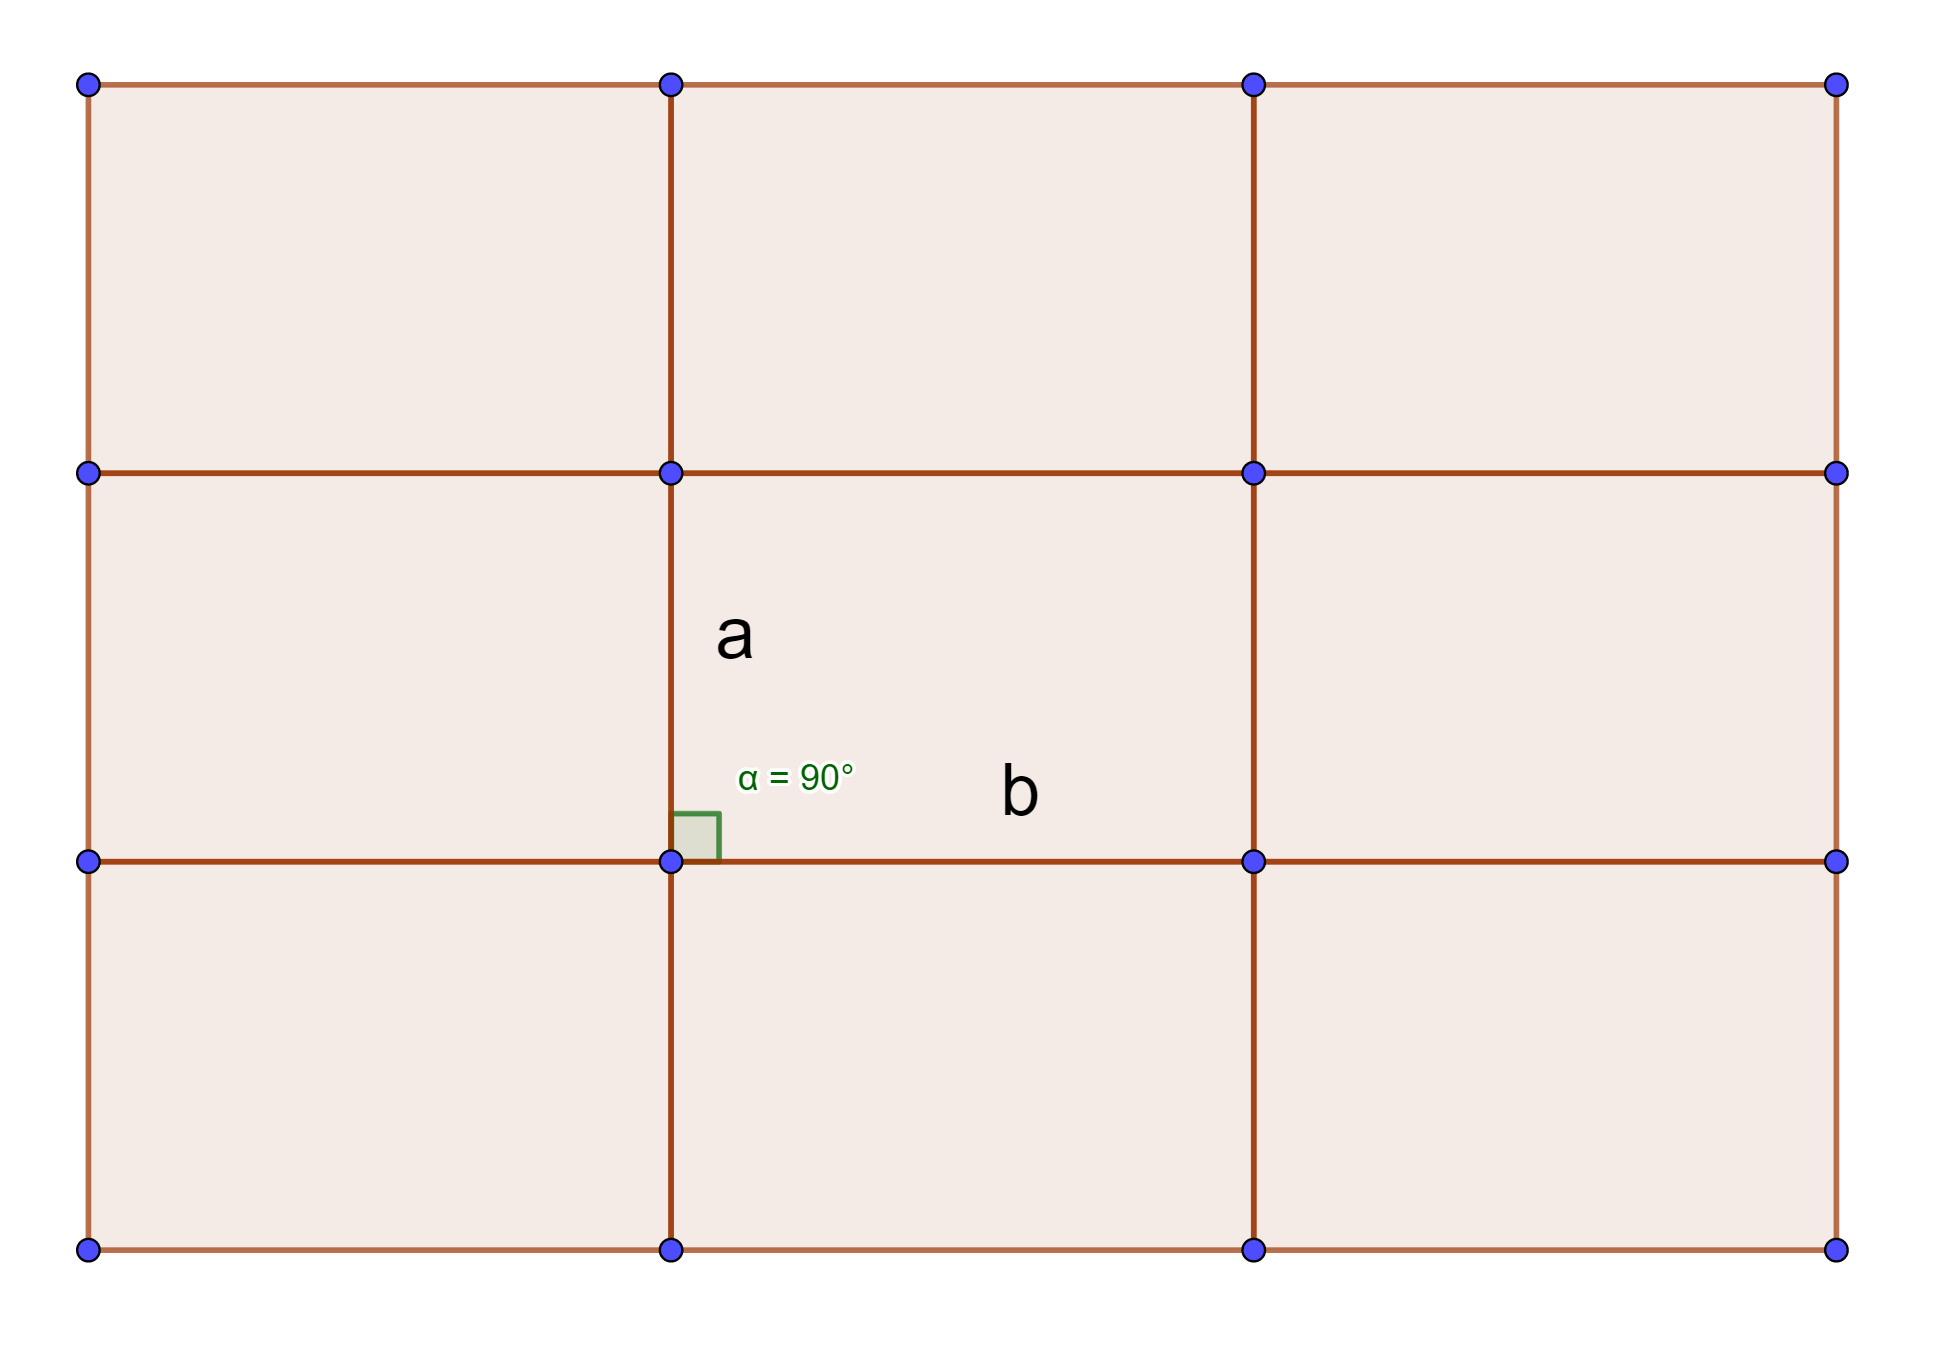
\includegraphics[width=0.4\textwidth]{./pic/p008-2.png}
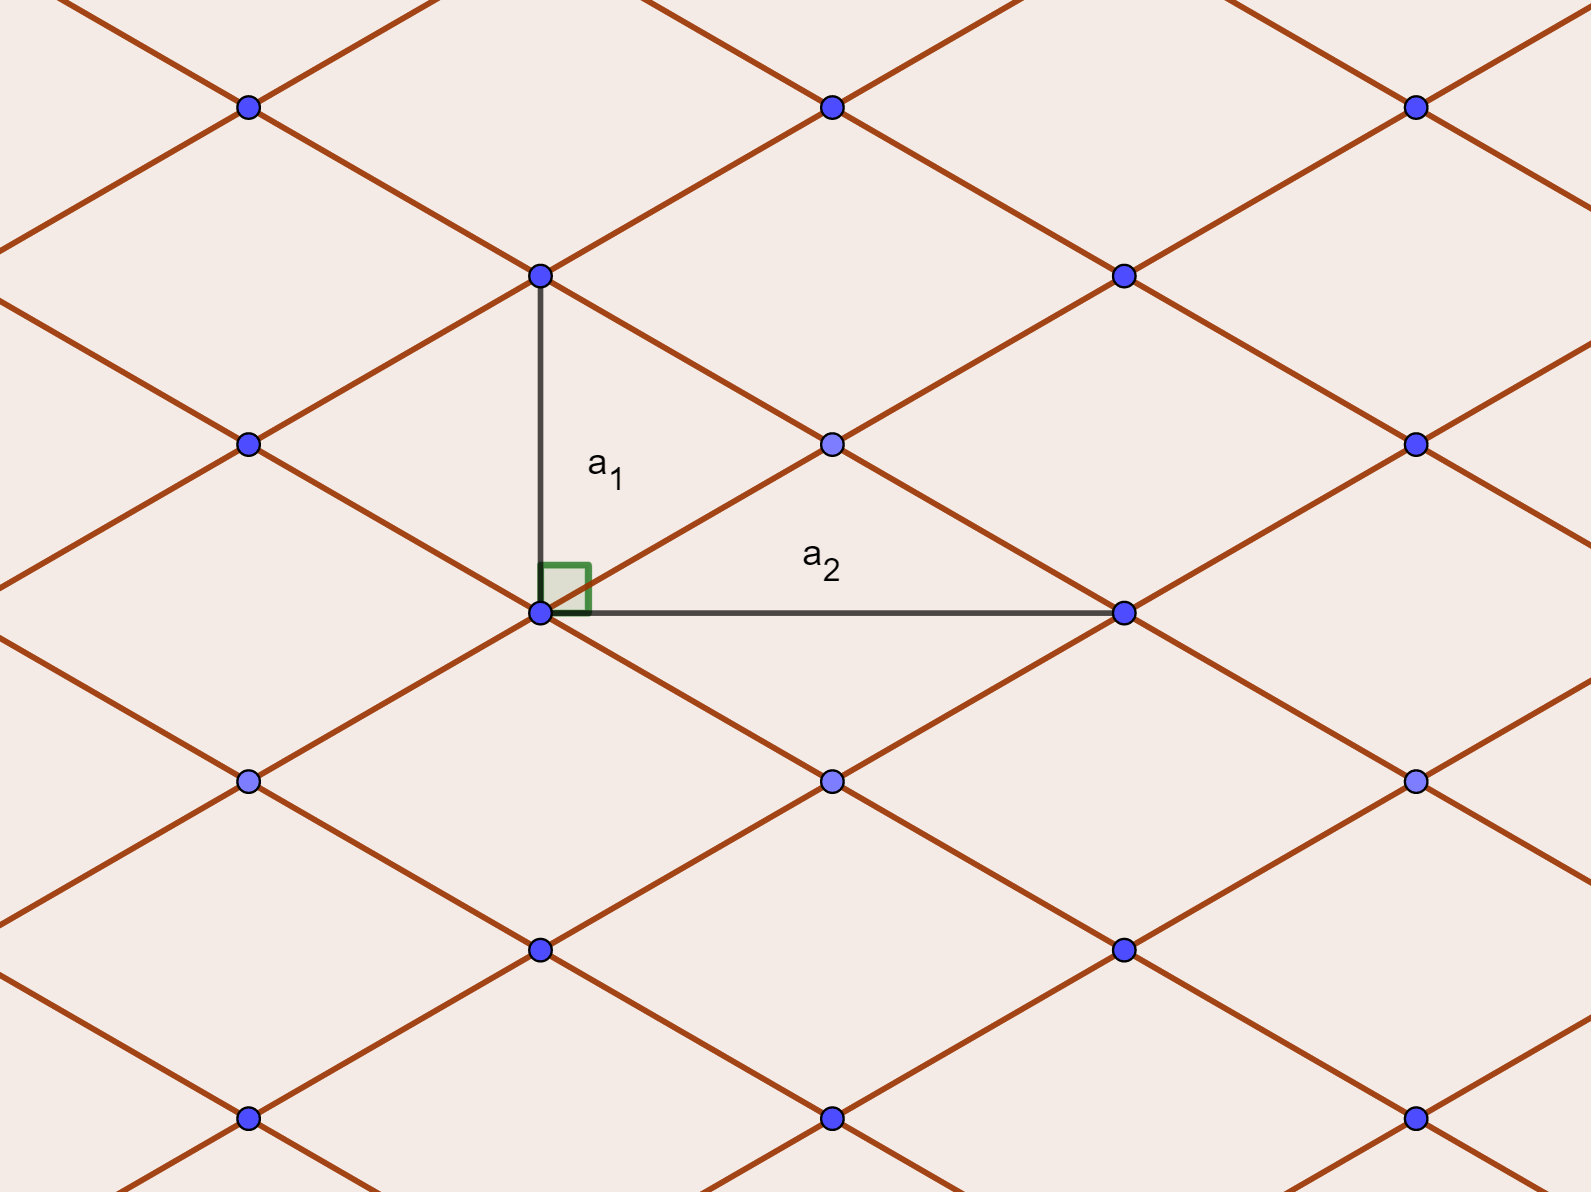
\includegraphics[width=0.3\textwidth]{./pic/p008-3.png}
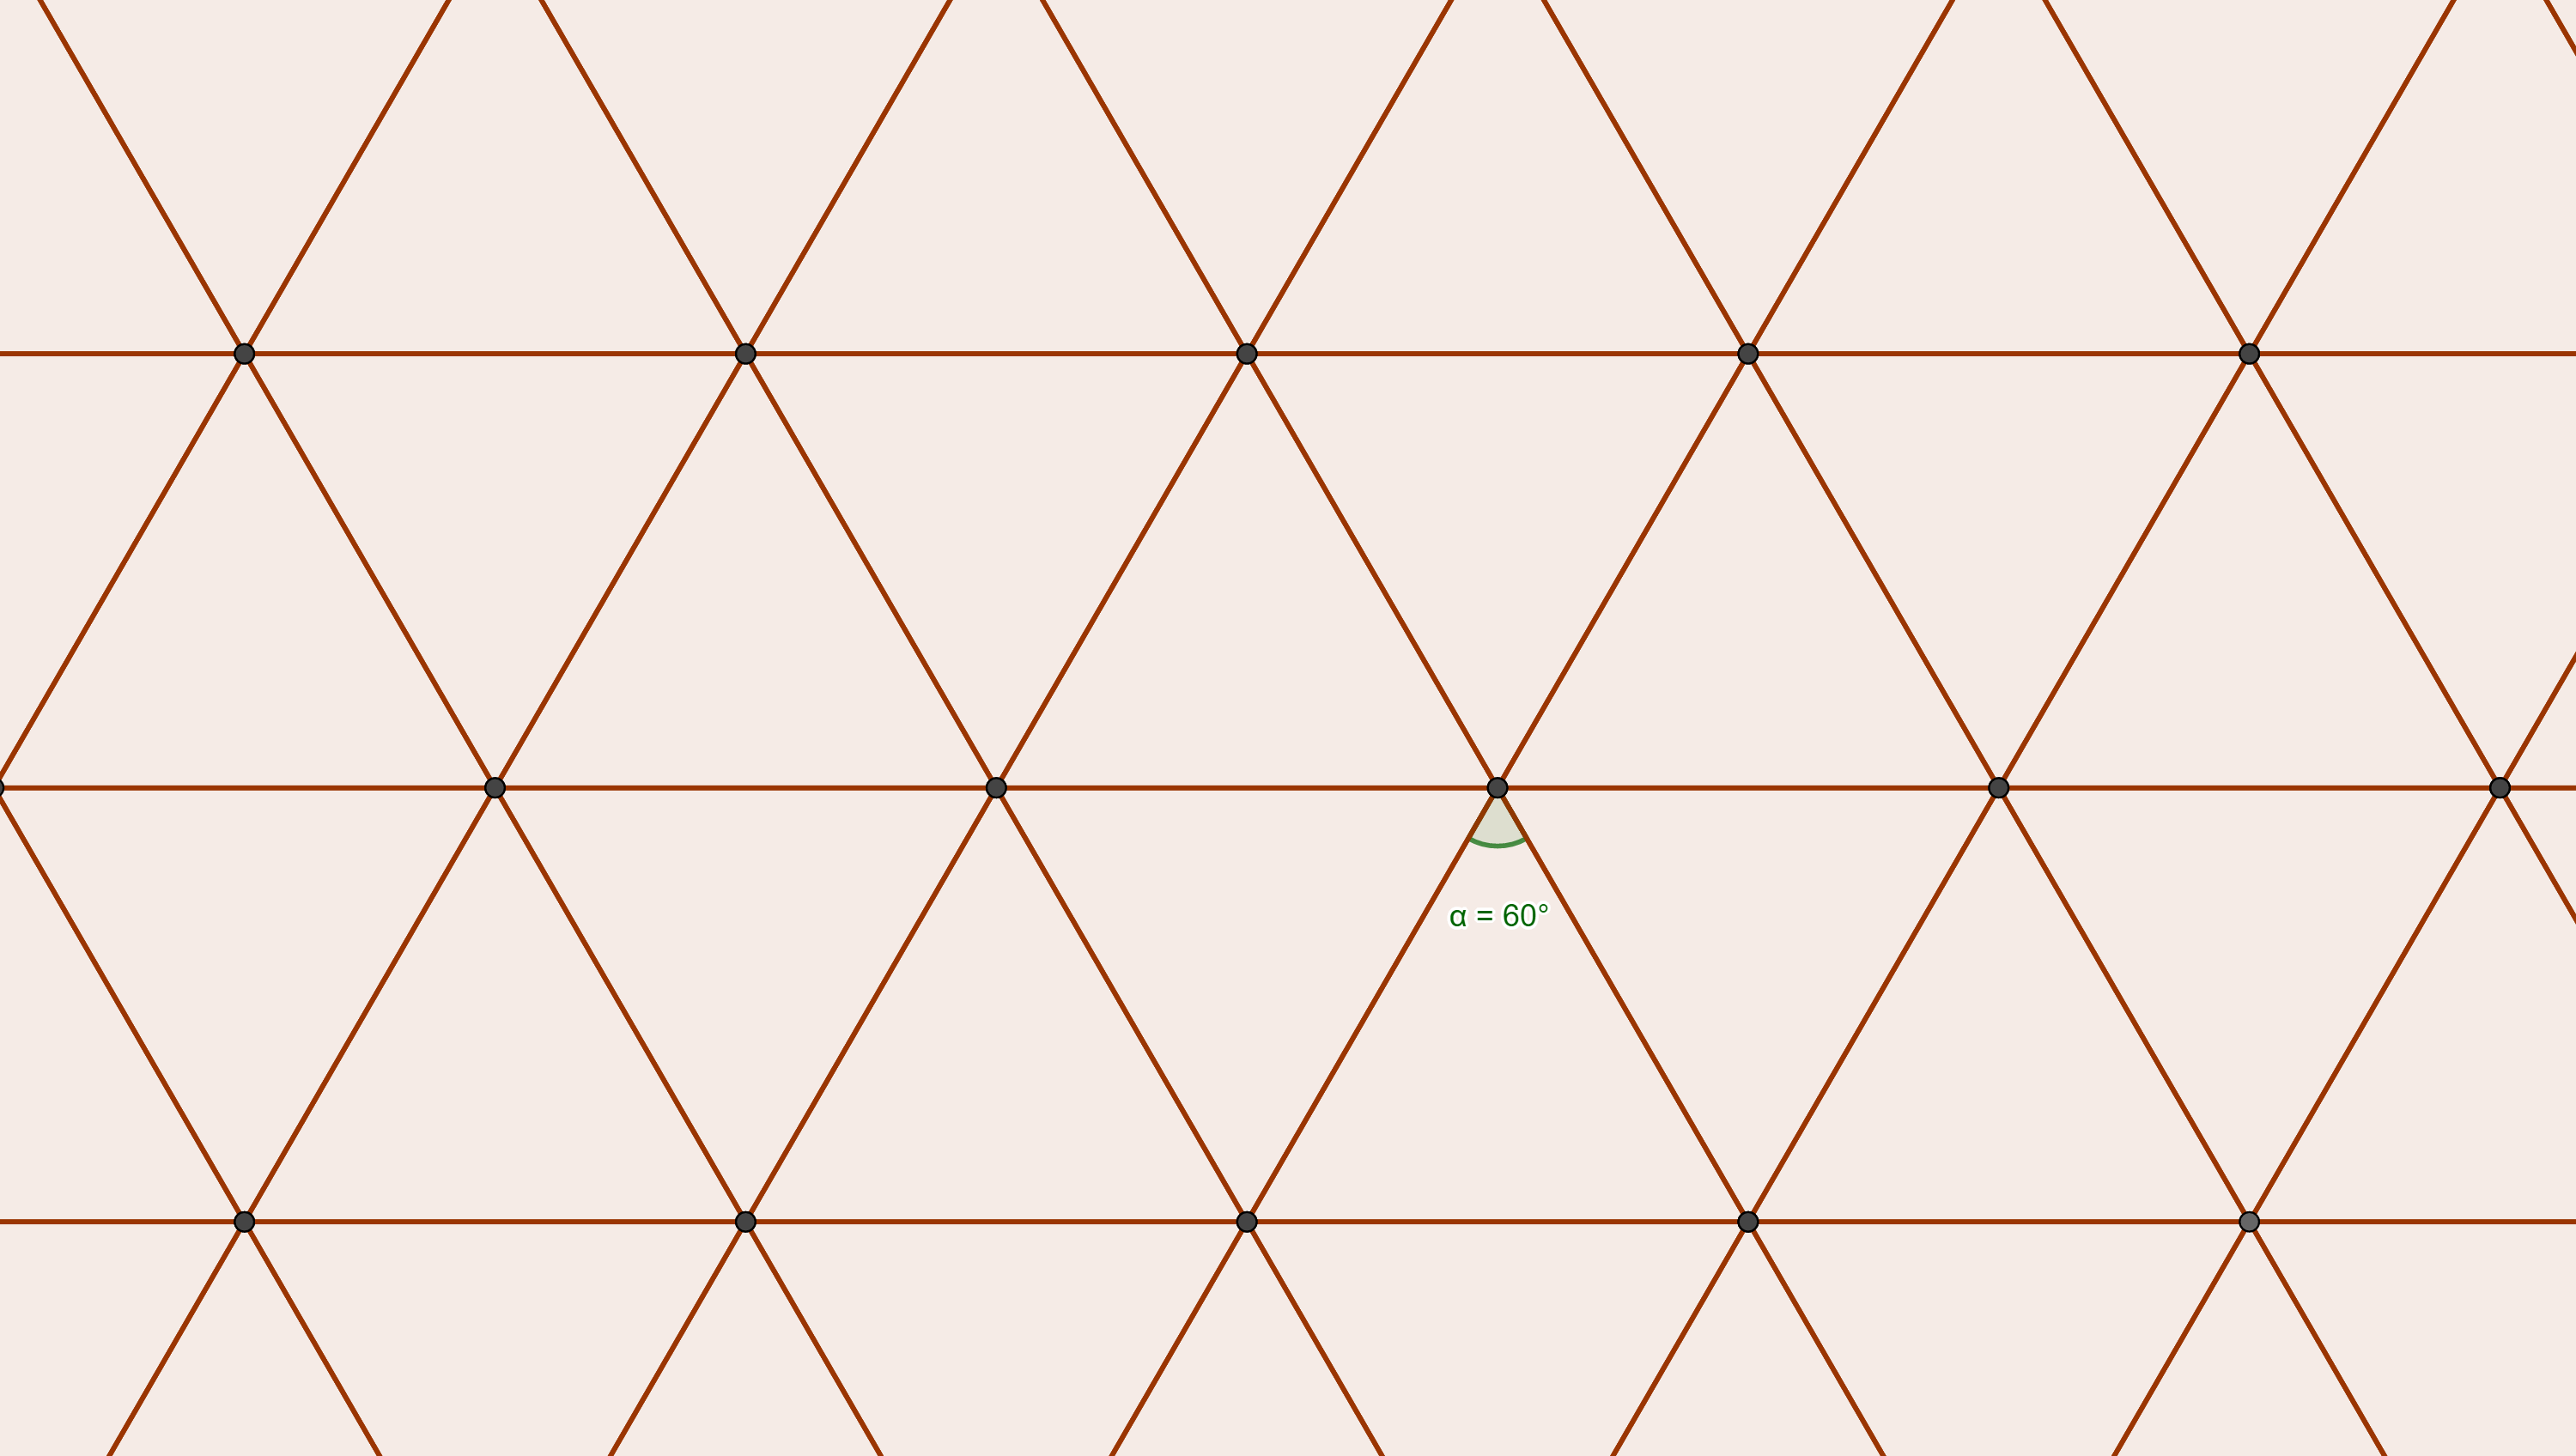
\includegraphics[width=0.3\textwidth]{./pic/p008-4.png}
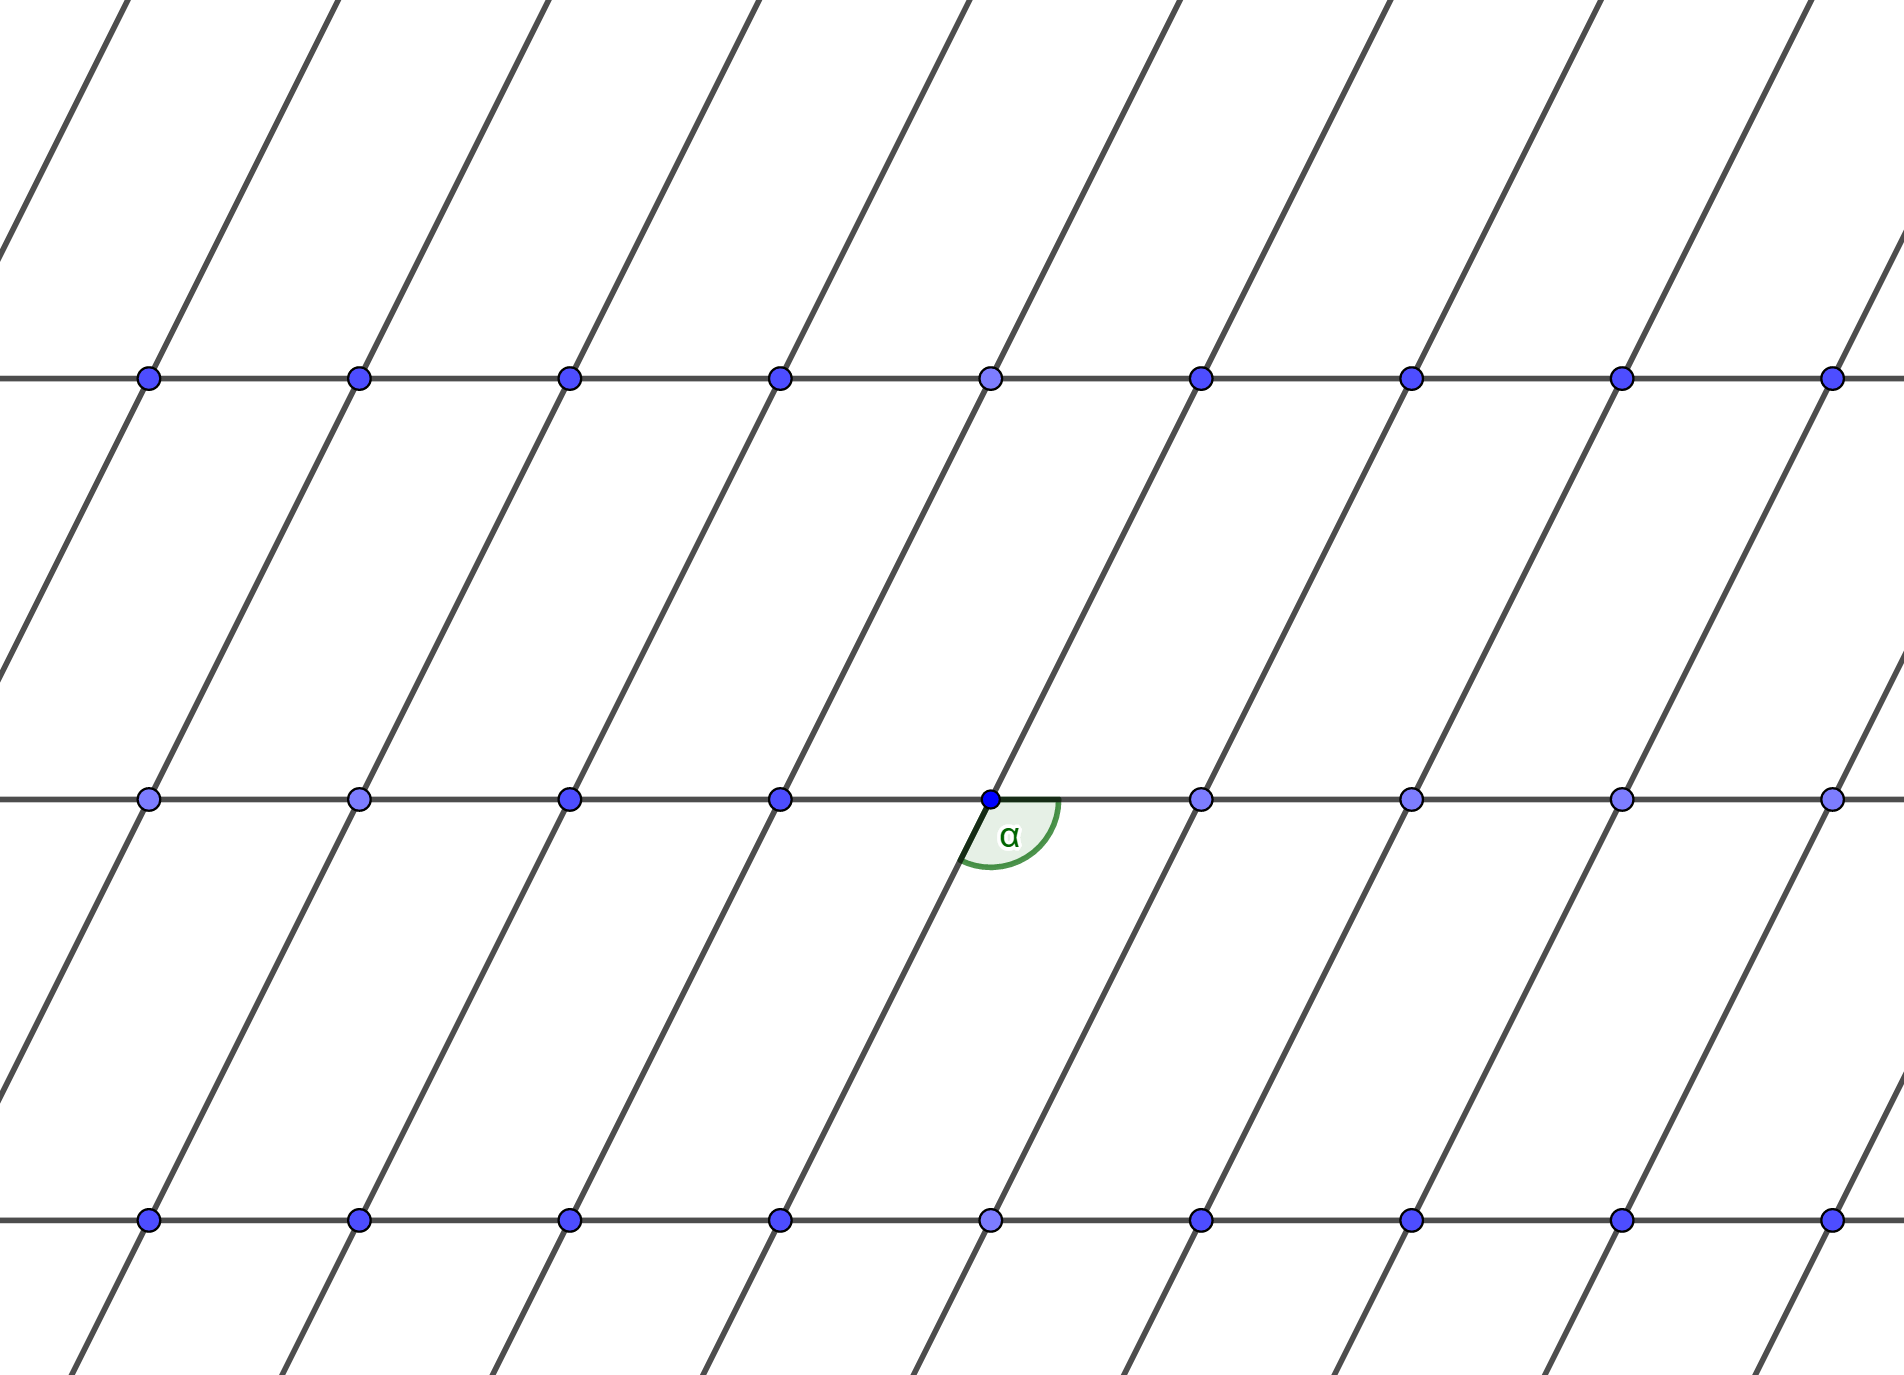
\includegraphics[width=0.3\textwidth]{./pic/p008-5.png}

\caption{二维空间中的五种布喇菲格子}

\label{dogp08}
\end{figure}
% \end{document}






\chapter{多铁材料的应用与发展前景}

\section{多铁材料的应用}
多铁材料在各个领域都有着及其重大的应用前景,尤其是在信息存储领域。利用多铁材料铁电铁磁耦合的性质可以制作“磁读电写”存储器,实现高可靠性、低能耗、高速度存储。

% \begin{itemize}
%     \item 多态存储器
    
%     多铁材料同时拥有铁磁性与铁电性两种性质,用这两种性质的四种组合可以存储数据,存储密度比传统的磁存储存储密度有着巨大的提高。

    
%     \item 低能耗逻辑存储器
%     \item 磁电探测器
%     \item 高频射频器件
    
% \end{itemize}
\paragraph{多态存储器}
多铁材料同时拥有铁磁性与铁电性两种性质,用这两种性质的四种组合可以存储数据,存储密度比传统的磁存储存储密度有着巨大的提高。
与传统的磁存储与电存储相比具有两种铁性质的多铁材料无疑在信息存储技术方面会占有巨大的优势。通过外加电磁场的调控,可以实现四种阻值的状态,通过合适的工业技术手段,可以实现对存储效率的倍增。

\paragraph{低能耗逻辑存储器}
目前寻求更高效的低能耗存储器是计算机技术的一个重要的发展方向。现在的发展趋势是将自旋霍尔效应与多铁材料的电场调控磁性相结合,制成多铁性的包含强自旋轨道耦合的逻辑存储器。通过自旋霍尔效应可以将自旋转化为电荷或者电场,而多铁性的铁电铁磁耦合可以利用电场调控磁性或自旋,如果这样的存储器可以研制成功,器件整体工作电压将从5V左右降低到100mV,反转或存储一比特信息所需要的能量将有希望降低到1aJ。就目前来说,在众多发现的材料之中,最古老的多铁材料$BiFeO_{3}$希望最大。




\paragraph{高频射频器件}
高频射频器件也是多铁材料的重要应用方向之一。高频射频器件在无线通信、国防军事等方面有着重大应用价值,就目前研究来看,此方向应用最多的是基于机械耦合的多铁材料。

\paragraph{磁电探测器}
多铁性材料最直接的应用之一就是磁电传感器,多铁材料内部铁电性与铁磁性相耦合的性质可以很容易地实现电信号与磁信号的相互转化。相对于传统的磁电传感器,基于多铁材料电磁耦合效应的磁电探测器在工作时不需要消耗能量,可以做成无源器件,对简化电子电路有很大价值。
\begin{figure}[h]
    \centering
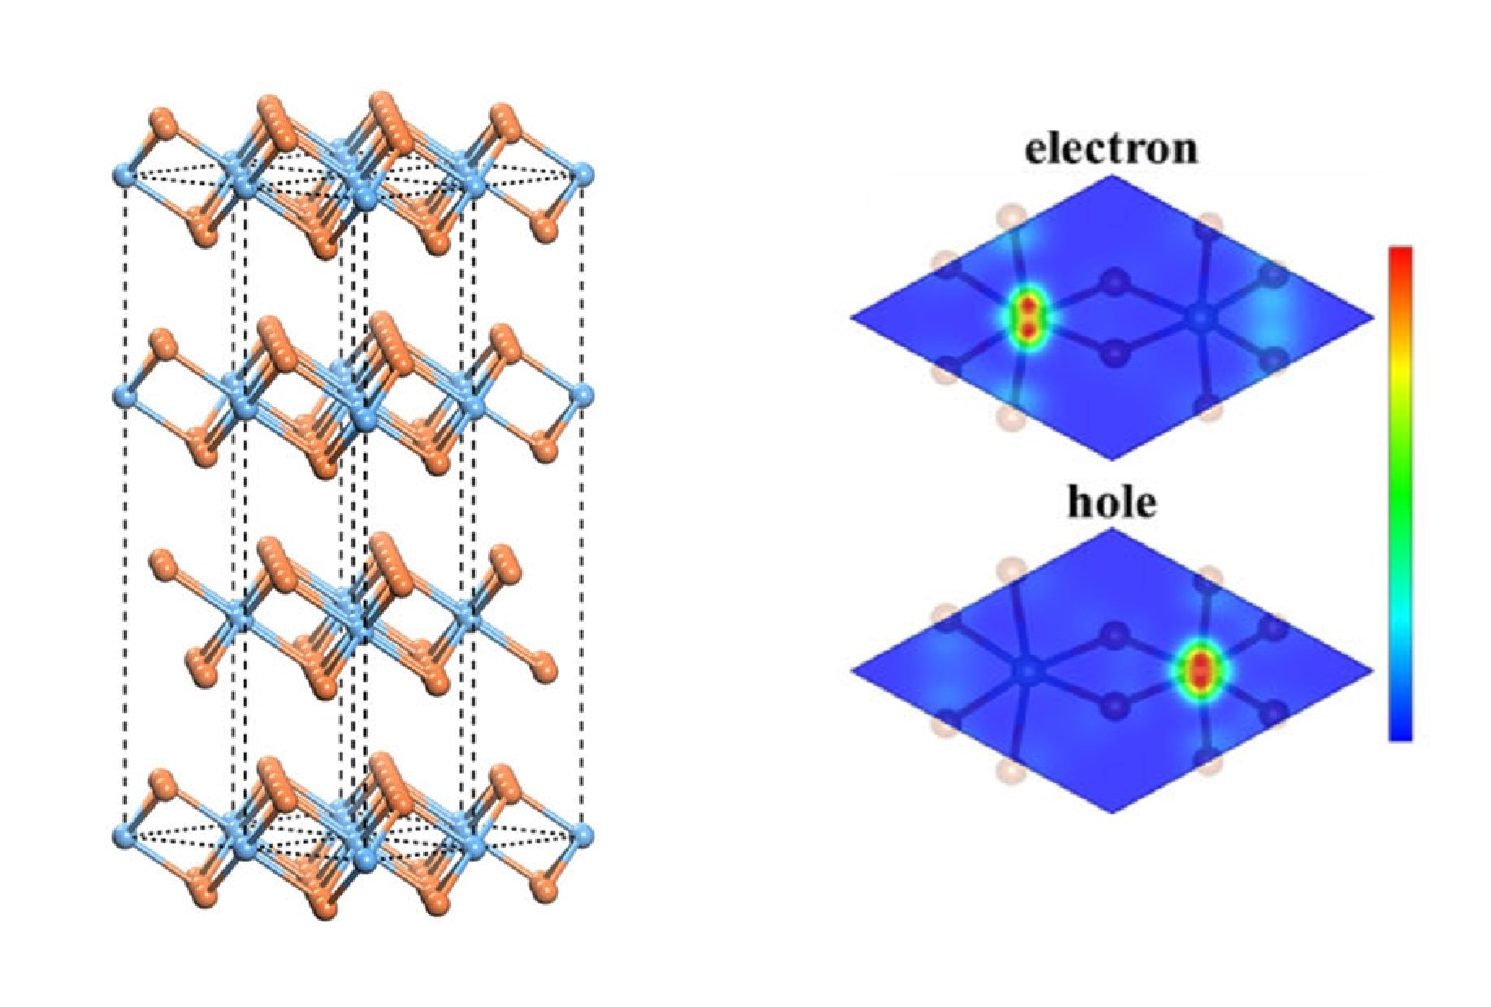
\includegraphics[width=0.8\textwidth]{./pic/010-4.png}
\caption{层状溴化铬结构与溴化铬掺杂电子或空穴后的电子密度分布变化。}

\label{dog010-4}
\end{figure}


\subsection{多体材料研究的展望}

有待解决的若干重大问题与相关要点:
\begin{itemize}
    \item 发现一种室温强耦合的新型多铁材料\\
目前发现的多铁材料都有或多或少的缺点,距离现实实际的生产生活仍然有着一定的距离。为了达到应用的目的,仍然需要寻找出室温下稳定性高,电磁性质关联度高的多铁材料。寻找能广泛应用的多铁材料是贯穿整个多铁材料研究的重要目的之一。
    \item 利用原子尺度设计与逐层生长技术相结合,改良现有的多铁复合材料\\
随着新的实验与理论工具的不断成熟与发展,原子尺度设计与逐层生长技术成为制备寻找新型使用多铁材料的重要手段之一。
    \item 发展并提出新的电磁耦合机制,探索与接近理论极限 \\
从当今对多铁材料的研究看来,还是没有一种完美的对多铁性质的通用解释。随着人们对多铁材料的实验积累越来越多,对多铁材料的认识越来越深入,需要新的更合适的理论方案来解释新的实验现象与对新材料进行理论计算预测。
    \item 理解控制与应用铁磁铁电转换动力学\\
多铁材料研究的核心之一是多铁材料内部铁磁性与铁电性的耦合关系与具体实现机制,磁相互作用与电相互作用的转换动力学是研究的关键点之一。
    \item 多铁性在物理学其他领域的现象与作用\\
多铁性材料在凝聚态物理的其他领域或许有着其他新现象或者作用。
\end{itemize}

\begin{figure}[h]
    \centering
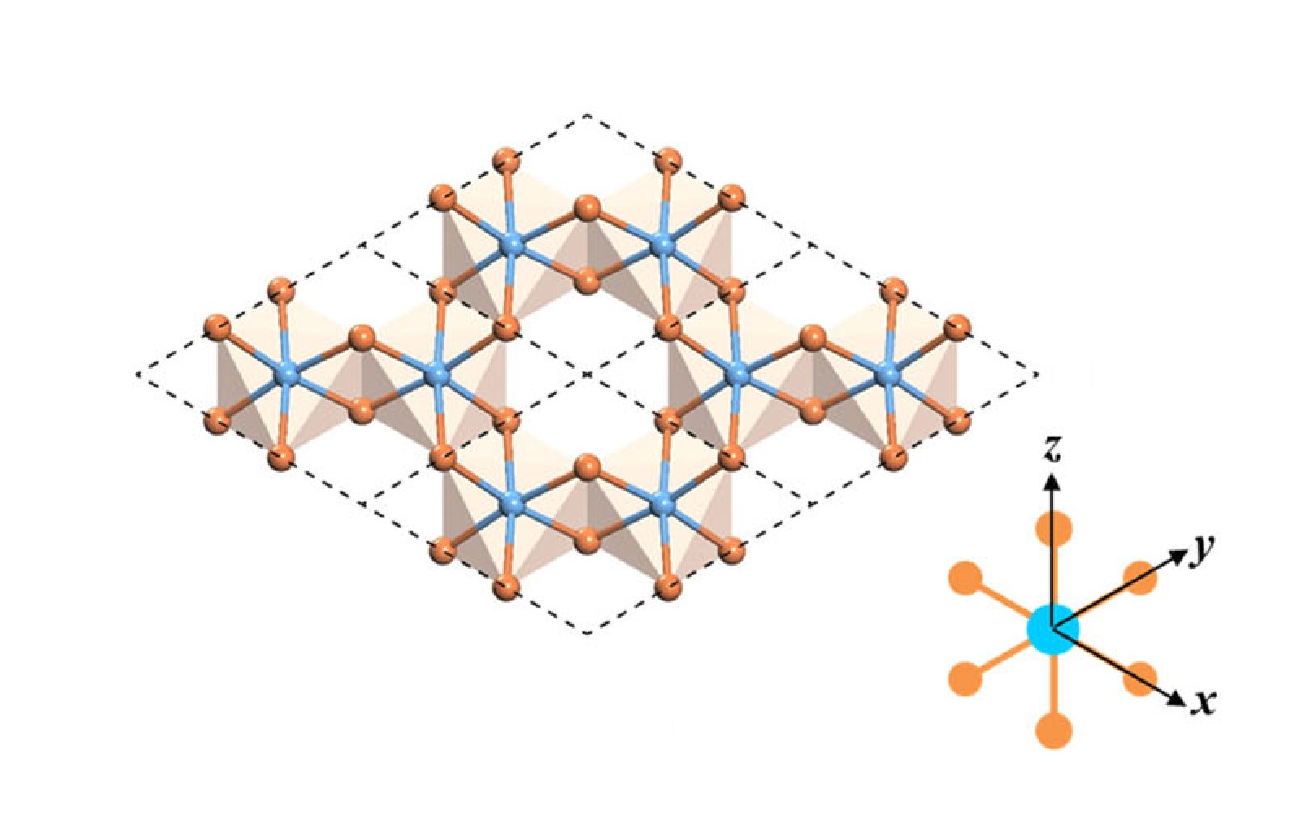
\includegraphics[width=0.8\textwidth]{./pic/010-2.png}
\caption{二维溴化铬微观结构\ 每个铬离子与周围六个溴离子相连,一个溴离子与两个铬离子相连。铬离子在空间平面中构成六边形网状结构。}

\label{dog010-2}
\end{figure}

\section{材料理论计算的新方法与发展}

\subsection{高通量计算材料学}

随着先进的自动化计算技术的进一步完善与发展,通过计算预测、发现、设计新材料的准确度、可靠性、计算效率进一步提高,近年来,随着机器学习等计算机技术的发展,利用数据挖掘进行高通量筛选新材料研究越来越受到重视。以二维材料为例,利用自动化工具可以在已知的材料里面筛选出二维材料。进行数据材料筛选,首先需要有一个筛选范围,通常是完备的晶体学数据库。由于二维材料等低维材料层状结构之间存在着巨大的空隙,其原子的共价体积与晶格原包的体积之比比较小,首先将填充比在0.15~0.50筛选出来。然后再筛选层状结构的层间距离较大的材料,最后在检查层状结构之间有没有共价键穿过。这种筛选方法固然会漏掉一些材料,但可以筛选出大部分的二维材料。

\subsection{演化算法}

随着现代计算机技术的发展与进步,理论计算在发现新材料的过程之中起着越来越重要的作用。在计算机科学落后的过去,计算能力的有限限制了采用大规模计算的方式进行材料筛选的方式,只能在实验上采取试错法等低效率的方法进行,在这个过程之中,新材料的能否发现与发现过程是否顺利在客观实验条件之外主要取决于实验参与人员的经验与熟练程度。到了计算技术成熟发展的今天,利用理论计算工具对材料进行初步筛选大大加快了新型材料的发现与实验成功率。

利用计算机技术对众多材料结构进行预测的核心问题是找到以众多参数为因变量的目标性质参数函数的全局最小值,由于材料类型多种多样,结构种类各异,组成元素千奇百怪,对所用的可能的元素组合与结构变化全部计算一次是显然不可能的,必须利用一些特殊的技巧对计算过程进行简化。目前已经存在多种有效方法进行结构预测,主要有:遗传算法、随机取样、微分演化算法、模拟退火等方法。其中演化算法是一种比较有代表性的算法,可以分为五个步骤:产生初始结构、结构弛豫、相似性分析与适应度函数、产生新结构、收敛性判断等五个步骤。

\subsubsection{初始结构}

初始结构是演化算法预测新材料的第一步,为了减少不必要的计算通常应该从晶格结构的对称性方面考虑并对原子位置加以限制,对于二维结构来说,分别对应17个平面群与80个层空间群。一旦一个原子的位置确定之后,其对称性位置可以通过空间群的点群矩阵和平移矢量得到:
\begin{equation}
    \begin{split}
        \tilde{ x}_{1}= W_{11}x_{1}+W_{12}x_{2}+W_{13}x_{3}+\bm{w}_{1} \\
        \tilde{ x}_{2}= W_{21}x_{1}+W_{22}x_{2}+W_{23}x_{3}+\bm{w}_{2} \\
        \tilde{ x}_{3}= W_{31}x_{1}+W_{32}x_{2}+W_{33}x_{3}+\bm{w}_{3} \\
    \end{split}
    \label{eq:jg}
\end{equation}
在通过点群的周期性结构平移之后,还需要加上若干硬性的限制,以使得所构造的结构符合物理事实,包括不限于以下限制:原子间的最小距离、在给定原子数目下晶格的大小等。具体的限制要结合所研究的条件尺度体系等具体设置。

\subsubsection{结构弛豫}

几何结构弛豫在第一性原理计算方面已经发展成熟,各种软件都有着成熟的体系来进行结构弛豫,通常采用的方法有最速下降法、准牛顿法、共轭梯度法等相关方法。进行结构弛豫之后不仅可以优化结构及其能量,还可以得到结构的一些其他性质,并且可以为下一步的结构相似性分析提供数据支撑与前提条件。

\subsubsection{相似度分析与适应度函数}

在结构弛豫之后,会有大量的大量结构优化到统一构型,如果不加以甄别会造成大量的重复计算,从而降低结构的多样性与寻找新结构的效率。为了解决这一问题,需要进行相似度分析,通过定义相关结构的数学特征量可以定量导出两种结构的相似度,通过对高相似度结构的合并与归类,可以大大减少不必要的计算。比较常用的一个原子键加权平均指标为:
\begin{equation}
    \bar{Q}_{lm}^{\delta_{AB}}=\frac{1}{N_{AB}}\sum_{i \in A,j \in B}e^{-\alpha(r_{ij}-b_{AB})}Y_{lm}(\theta_{ij},\phi_{ij} )
    \label{eq:jjq}
\end{equation}

其中$Y_{lm}(\theta_{ij},\phi_{ij} )$是球谐函数,与两个原子之间的相对位置有关,$\theta_{ij}\text{和}\phi_{ij}$是化学键的方位角,$\delta_{AB}\text{和}N_{AB}$分别是键的类型与数目。考虑上参考系变换的不变性,可以对m进行求和:
\begin{equation}
    Q_{l}^{\delta_{AB}}=\sqrt{\frac{4\pi}{2l+1}\sum_{m=-l}^{l}|\bar{Q}_{lm}^{\delta_{AB}}|^{2}}
    \label{eq:jjq2}
\end{equation}
这样就可以得到不同键的特征值,最终组成键结构的特征矩阵,利用这一矩阵可以定义两种结构之间的差异:
\begin{equation}
    D_{UV}=\sqrt{\frac{1}{N_{type}}\sum_{\delta_{AB}}\sum_{l}(Q_{l}^{\delta_{AB},U}-Q_{l}^{\delta_{AB},V})^{2}}
    \label{eq:jjq3}
\end{equation}

通过相似性筛选之后,需要对这些不同的结构进行筛选,选出“好”结构,一般是选择能量最低,比较稳定的结构,如果对材料的某种功能进行逆向设计,则需要采用其他的标准进行分类评判。

\subsubsection{产生新结构}

利用原有的结构经过一系列的操作产生新的结构,是演化算法的一大特点。产生新结构的首要问题就是选取那些老结构作为新结构产生的依据。截断法是一个比较经常采用的方法,取某种指标的一个定值作为标准,只选取达标的部分。组合法划分为多个小组,在各个小组内部分别选择。随机法是在指标的基础上加上随机数的影响。以上的方法也可以混合使用,随机数的引入可以增强结构的多样性。产生新结构的方法也有很多种常见的有遗传算法、粒子群优化算法和微分演化算法等方法。

\paragraph{遗传算法}遗传算法一般采用混合和变异来产生新的结构。以二维材料为例,在若干结构内部划分为多个部分,在不同结构中随机选取并交换一部分,在进行必要的调整之后可以作为新的结构供应下一代使用。变异方法是大范围引入随机性,可以随机改变原子位置,随机改变原子种类,随机改变晶格结构。以二维材料为例,可以通过下面的变换矩阵进行随机微调:
\begin{equation}
    [\bm{I}+\epsilon_{ij}]=
    \begin{pmatrix}
        1+\epsilon_{11}&\frac{\epsilon_{12}}{2}&0\\
        \frac{\epsilon_{12}}{2}&1+\epsilon_{22}&0\\
        0&0&1
    \end{pmatrix}
    \label{eq:yc}
\end{equation}
其中$\epsilon$是随机数。随机数的引入有助于保持结构的多样性,对搜索低能结构附近的势能面非常重要。

\paragraph{粒子群优化算法}粒子群优化算法来源于仿生学,主要受到自然界的群体生物的群体活动智能系统的启发。在某些自然界的生物组群之中存在着广泛的自组织行为。在众多仿生学算法之中,粒子群优化算法是其中一个重要的算法。
\paragraph{微分演化算法}
微分演化算法的核心是考虑不同之间差别,其通用表达式为:
\begin{equation}
    p'_{i}=\gamma p_{best} +(1-\gamma)p_{i}+F(p_{r1}-p_{r2})
    \label{eq:sf}
\end{equation}
其中$p_{r1}\text{和}p_{r2}$是母代之中随机选取的两个个体,针对具体问题的操作还是要结合实际情况考虑。

\subsubsection{收敛性判断}

判断结果是否收敛是整个计算过程的最后一步,根据遗传算法的原理,计算可以无穷无极迭代下去,但这显然是没必要且不可能的,为了尽可能减少计算量与得到结果,通常需要设定一个收敛判据。判断方法有很多种,最直接的一种是如果计算多代之后效果没有明显提高,即可认为结果已收敛,可以结束计算了。

\subsection{机器学习}

随着现代计算机技术的发展与进步,以薛定谔方程与密度泛函理论为基础的计算方法在凝聚态物理、材料科学与计算化学中发挥着越来越重要的作用。计算机技术这一重要工具与手段对基础学科的发展有着巨大的促进作用。在二十一世纪,机器学习这一新兴的计算机技术开始在各个领域发挥作用,将机器学习等人工智能技术与手段在计算材料领域也有着巨大的应用前景。机器学习与人工智能技术作为一种新兴手段在很多领域可以取代人类做一些重复性的工作,越来越多领域开始采用这种方法来进行辅助工作,随着机器学习应用范围越来越广,机器学习技术应用的资源和工具意味着进入的障碍比以往任何时候都要低。

\begin{figure}[h]
    \centering
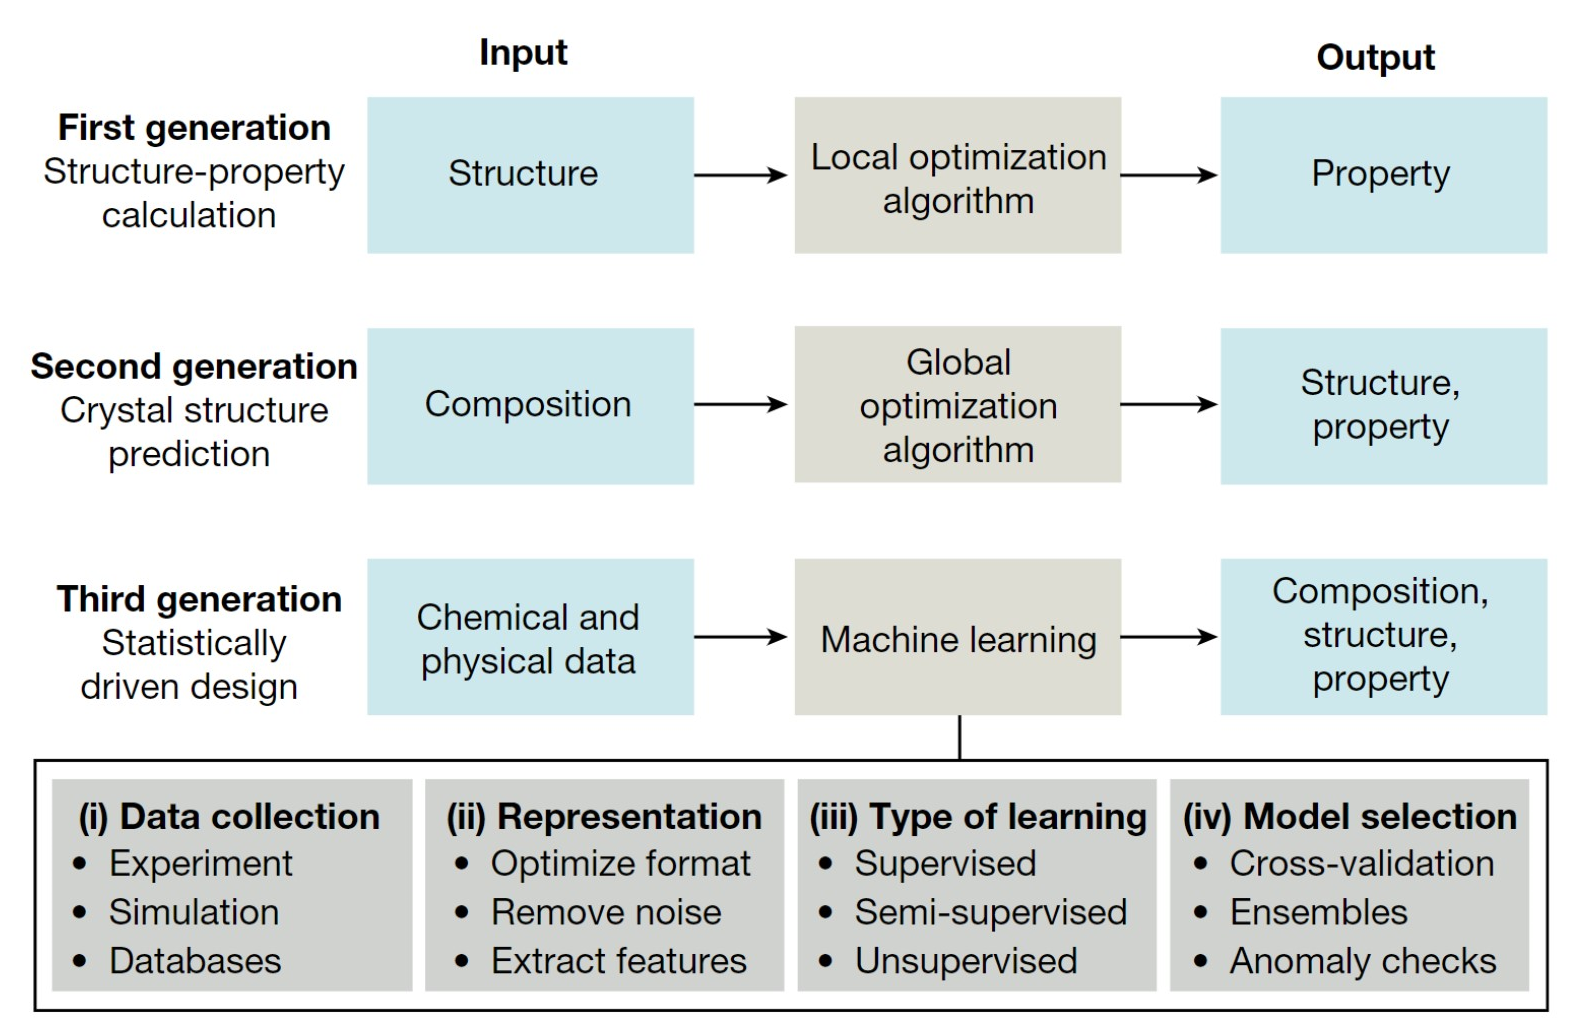
\includegraphics[width=0.8\textwidth]{./pic/025.png}
\caption{计算材料学的三代方法 \ 第一代方法是输入物质的物理结构,通过第一性原理计算等方式导出物质的性质,并通过结构与性质的对应关系来实现新材料的发现与设计。第二代采用全部据优化方法,输入物质的组成,通过一系列算法输出结构与性质。第三代是通过机器学习,输入基础的物理化学规则与数据,全自动地输出材料的组分结构与性质。机器学习的方法自动化程度更高,但是其计算过程难以理解与解释。}

\label{dog025}
\end{figure}

机器学习等方法并不是万能的,相关的模型参数等也不会凭空产生,机器学习的方法需要足够多的数据。只要有足够多的数据与合适的规则发现算法,计算机就可以确定已知的或者尚未发现的规律。与传统计算方式相比,机器学习方法主要通过学习数据的一部分并自动化建立模型来拟合数据的另一部分,通过优化后的模型来辅助解决实际问题。

\subsubsection{机器学习在计算材料学应用的一般方法}

\paragraph{收集数据}
数据是机器学习的核心之一,是决定工作成败的一个重要因素。数据不会凭空产生,足够多的准确数据是机器学习的前提条件。虽然现在有很多晶体学数据库,但并不能直接拿来作为数据源,需要结合实际问题从数据库中挑选出合适的数据。

所需要数据的类型结构与数量与所选取的学习方法也有关系,通常的学习方法有监督学习、半监督学习与无监督学习。有监督学习包含输入与输出,目的是根据输入数据产生一个具有相当可信度的输出预测值,这类数据需要输入与正确的预测值。无监督学习通常不需要进行输出,一般用来进行识别数据中的趋势、模式与聚类。半监督学习主要应用在输入数据远多于输出数据的情况下,通常可作为数据生成器使用。

\paragraph{数据预处理}
找到正确合适的数据集之后并不能直接拿来用,需要对数据进行预处理,对数据中的错误与噪声等对下一步造成障碍的不利因素要剔除出去。从各种途径采集到的原始数据并不一定总可以适应算法,适当对数据进行预处理,将数据从一种形式转化为另一种更合适的形式可能大大加快机器学习的进程。

理论上看来,数据与算法适应程度越高,进行机器学习的效果会越好,但实际上人们很难明确给出最适合的数据形式,只能猜测出一个大概符合的数据形式。在研究分子问题时,库伦矩阵可以很好概括原子核周围的势能信息,而且在平移与旋转分子时也是不变的。在周期结构中,由于晶格对称性与周期性,传统平移向量与分数坐标等方法并不总是合适,因为可以通过选择不同的坐标系以无数种方式表示晶格。在表示周期性结构的晶格时通常采用径向分布函数等方法。

\paragraph{选择算法}

选择完成合适的数据集之后,下一步就是选择合适的算法,就像数据预处理的方式要与算法相适应一样,数据集也应该与算法相适应。有些问题比如分类等,需要分立值输出,所选取的经过预处理之后的数据集也应该是不连续的,对于另一些问题,例如预测性质,所输出的是连续值,所采用的数据集也应该是连续的。在处理复杂问题时,单一的学习算法效果不一定好,有时候则需要将多种学习方式融合起来,组成更复杂的学习组合。常见的算法有:贝叶斯分类器、k近邻法、决策树方法、支持向量机。人工神经网络等方法。其中目前最为流行的是人工神经网络方法,这种方法是一种仿生学方法,起源是对大脑功能与结构的简单模仿。其数据处理功能的人工神经元可以分为输入层、输出层和隐藏层。神经元接受其他神经元传递的信息,经过简单计算之后传递给其他神经元。神经元之间的连接权重存储着整个网络学习到的知识,神经网络学习训练的过程实际上是调整优化权重的过程,这个过程类似于回归拟合预测,通过调整各个参数使得输出最优结果。

\paragraph{模型优化}
在选定合适的算法之后,还需要在计算过程之中进行微调,以使得所建立的模型更加接近真实情况。在进行机器学习的过程之中,经常会出现一些偏差,这些误差主要来源有三种,模型偏差、模型方差与不可约误差。模型偏差主要是由于模型自身问题造成的,模型与真实的物理过程存在着系统性的偏差。模型方差是指对输入数据的微小变动引起输出数据的剧烈波动。不可约误差通常是指由于训练数据中的噪声,测量限制,计算不确定性,或者仅仅是离群值或数据丢失而导致错误。通过对计算过程的适当调整可以减小模型偏差与模型方差。

模型偏差过大通常发生在模型复杂度不足以描述输入与输出值关系或者数据不足以支撑发现输入与输出之间的关系,而方差过大则发生在模型过于复杂,在处理输入输出关系时无中生有地臆造出并不存在的规则,这种情况通常叫做过拟合,其标志之一是在训练数据中正确率不断提高,而在测试数据中准确率不再提升或开始下降。在具体的操作过程之中应避免这种情况,可以用多组数据进行交叉验证来避免错误。

\begin{figure}[h]
    \centering
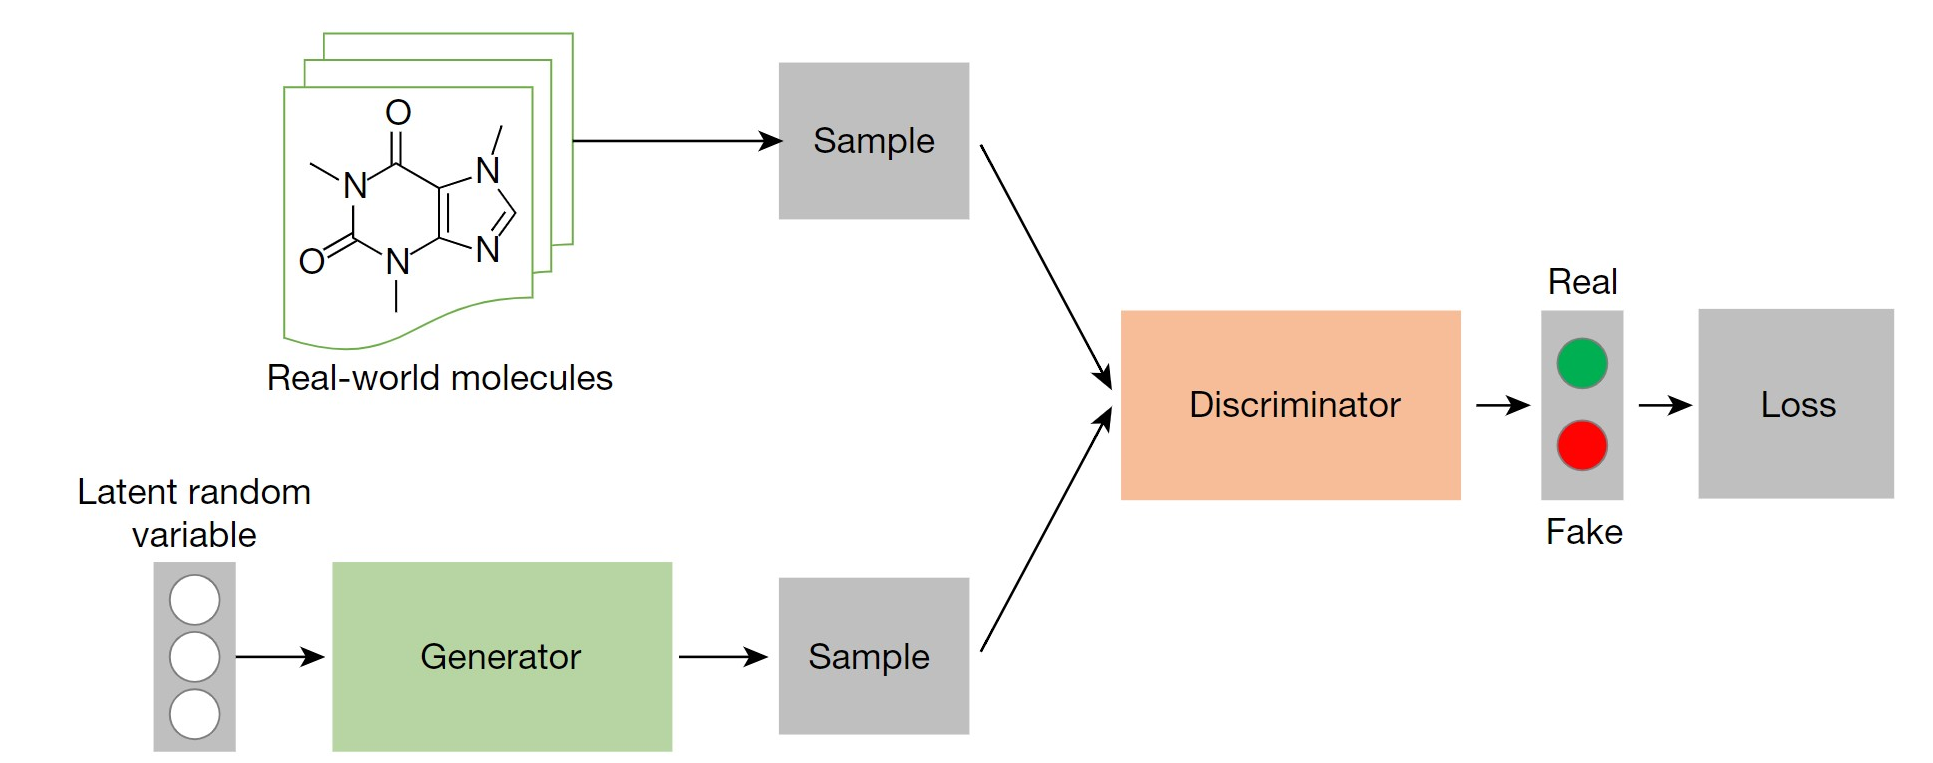
\includegraphics[width=0.8\textwidth]{./pic/026.png}
\caption{一种基于对抗生成网络的分子设计方法 \ 该方法是由两个网络做成的,一个生成器网络将随机数噪声转化为分子组合与结构,另一个判别器网络是将生成器网络造出来的分子结构与数据集中已知结构区分开,生成器的目的是使得所产生的分子结构不被判别器挑出来,而判别器的目的是选择出生成器产生的分子结构,两个网络相互对抗,协同学习,最终会使得输出结果接近真实的分子结构}

\label{dog024}
\end{figure}

\subsubsection{机器学习应用}

在材料领域,无论是理论计算还是实验领域,机器学习有着广泛的应用前景。机器学习可以用在指导化学合成,化学合成是一种很复杂的综合性问题,其应用型背景需要考虑成本、安全性、产率反应速率等多种因素。通过对文献中有机化学分子合成路线的学习,基于多层人工神经网络的深度学习方法设计出的有机物合成路线可以达到与人工专家无法区分的程度,但这种基于既有数据库的机器学习方法无法产生出超过已有知识体系的结果,即只能替代一些重复性的工作,无法进行创新性的工作。机器学习可也已进行一些数据辅助分析工作,在实验方面,应用不同的手段如X射线、中子衍射、核磁共振等对物质的结构与性质进行解析时会得到各有侧重的数据,每种方法都有其优点与局限性,机器学习方法可以用来发现多组数据之间的关联性。
% 通过对人工神经网络的学习与训练,还可以识别出物质相变时的过度
在计算大规模复杂系统时,机器学习可以代替DFT等传统第一性原理计算在可接受的误差范围内进行计算。随着计算化学数据库的不断增长,可以采用机器学习的方法以较小的计算成本实现较为准确的计算,相较于传统的第一性原理计算,基于机器学习的计算方法所消耗的计算资源要小很多。机器学习可可以应用于材料设计领域,尤其时逆向材料设计。预测给定成分晶体的结构是机器学习中有监督分类的重要应用方向。由于周期性结构晶体表示的多样性,现在的针对晶体的机器学习主要集中在有限的少数易于表示的结构上面,而针对单独的少数分子来说,这个问题就不复存在了,甚至可以通过生成对抗网络“创造”新的分子。随着时间的推移,越来越多的新材料极其性质被发现,在处理材料科学的文献方面,机器学习可以从论文当中提取出有效信息,自动识别出一段时间内的热点领域,甚至可以用来写论文综述。









\chapter*{结论}

本综述主要介绍多铁材料的研究背景与研究现状。多铁材料根据其铁电铁磁性质的来源与相互作用耦合强度可以简单的分为两大类,根据多铁性质的具体原理可以进一步细分。经过多年的发展,多铁材料的研究手段有了突飞猛进的进展,实验方面先进的观察手段可以从更小的时间分辨率与空间分辨率对多铁材料进行物理描述,在理论计算方面第一性原理计算依然是研究设计多铁材料的最佳方法。多铁材料的应用广泛,前途光明。多铁材料在基础研究上对研究铁磁铁电性微观原理有很大帮助。在应用层面电磁耦合的多铁材料可以在存储材料领域有重大价值,可以制造多态存储器、超低能耗存储器等。

多铁材料的研究范围也逐渐宽展到了二维材料领域,二维多铁材料研究的方法与一般的多铁材料相同。自从石墨烯问世以来,以二维材料为代表的低维材料逐渐成为研究热点。二维材料在空间结构上与三维体材料的巨大差别使得二维材料出现了很多新奇的物理特性。二维铁磁、铁电材料十分少见,二维多铁材料的发现之路也十分困难。到目前为止,所发现的性能良好的二维材料主要是第一类多铁材料。目前典型的二维多铁材料主要有过渡金属卤化物、双金属三卤化物等几种。其中基于过渡金属卤化物的二维多铁材料材料是通过对原有的二维铁磁材料进行电子掺杂,是材料内部同时出现电荷排序与轨道排序,进而产生电极化,使铁磁材料产生铁电性。而双金属三卤化物类材料则是具有天然存在的铁电性,通过两种铁电相之间晶体结构的差异使铁磁性在铁磁相与反铁磁相控制磁场,这种创新性的电磁耦合方式使得材料的电磁耦合强度接近第二类多铁材料,但实现通过磁场控制电场依然十分困难。

在二维多铁材料研究领域,第一性原理计算是研究的主流方法。基于密度泛函理论的理论计算工具在研究二维多铁材料上仍然适用,一些分子动力学方法也被应用在二维多铁材料某些性质的研究之中。到目前为止,寻找一种在室温下稳定的有着强电磁耦合的多铁材料仍然是二维多铁材料材料研究领域的首要目标。


\bibliographystyle{unsrt}
\clearpage
\phantomsection
\addcontentsline{toc}{chapter}{参考文献} 
\bibliography{dog.bib}

\chapter*{致谢}

2020年注定是不平凡的一年,也将是永载中华民族史册、人类发展史册的一年。年初一场新冠肺炎疫情突袭荆楚大地,蔓延波及全国以及全世界。在疫情发生之后,14亿中国人民在以习近平为核心的党中央坚强领导下,众志成城、团结一心,打响疫情防控的人民战争、总体战、阻击战。经过艰苦努力,付出巨大牺牲,湖北保卫战、武汉保卫战取得决定性成果,疫情防控阻击战取得重大战略成果,统筹推进疫情防控和经济社会发展工作取得积极成效。

受新冠肺炎疫情的影响,在这本科四年中的最后一学期,不能像往年一样在校园里进行毕业论文工作,而是在家里完成了这篇毕业论文。论文的大部分内容是在疫情最为严重的那段时间完成的,在那时,全国各地援助湖北武汉的医疗队才刚出发没多久,本地又出现聚集性疫情,面临着极大的扩散压力。与此同时,随着党中央“让党旗在防控疫情斗争第一线高高飘扬!”的命令下达,460多万个基层党组织、9000多万名党员迅速行动起来,成为抗疫中坚力量,铸就对抗新冠病毒联防联控机制的钢铁长城。自从看到小区门口防疫检查点上飘扬的党旗,我就明白并坚信在习总书记的亲自指挥下、在党的坚强领导下,中国人民一定会取得对抗疫情的人民战争的最终胜利。写下论文最后这一部分的时候已经是五月中旬了,此时湖北和武汉早已解封,境外输入疫情高峰已经过去,除了个别地区之外,全国各区县均为低风险地区。不容辩驳的事实证明了我在二月初的判断,更是又一次证明了在党的领导下,中国人民是不可战胜的,中国特色社会主义制度是中华民族攻坚克难、迈向复兴的根本保障。

% 在论文写作中,我要感谢赵明文老师的指导与帮助,使我能够顺利完成毕业设计,在此表示衷心的感激。\sout{还要感谢在论文写作过程中找我帮忙的同学,使我在论文的写作过程中以及在受新冠肺炎疫情影响下的居家生活中不会太无聊。}

在论文写作中,我要感谢老师的指导与帮助,使我能够顺利完成毕业设计,在此表示衷心的感激。\sout{还要感谢在论文写作过程中找我帮忙的同学,使我在论文的写作过程中以及在受新冠肺炎疫情影响下的居家生活中不会太无聊。}

在五四青年节前夕,习近平总书记寄语新时代青年强调“坚定理想信念站稳人民立场,练就过硬本领投身强国伟业”。一个时代有一个时代的际遇,一代青年有一代青年的使命。2020年是最不寻常的一年,在这百年未有之大变局来临之际,作为新时代的青年,我要牢记总书记的嘱托,不忘初心,牢记使命,把个人的理想追求融入国家和民族的事业中。

我们从哪里来?从深重的苦难与磨砺。

我们向何处去?向着民族复兴的光明未来。

任何磨难都只能激发我们奋斗的力量。

任何困难都不能阻挡我们前进的步伐!



 





\end{document}